\documentclass[american,]{article}
\usepackage{lmodern}
\usepackage{amssymb,amsmath}
\usepackage{ifxetex,ifluatex}
\usepackage{fixltx2e} % provides \textsubscript
\ifnum 0\ifxetex 1\fi\ifluatex 1\fi=0 % if pdftex
  \usepackage[T1]{fontenc}
  \usepackage[utf8]{inputenc}
\else % if luatex or xelatex
  \ifxetex
    \usepackage{mathspec}
  \else
    \usepackage{fontspec}
  \fi
  \defaultfontfeatures{Ligatures=TeX,Scale=MatchLowercase}
\fi
% use upquote if available, for straight quotes in verbatim environments
\IfFileExists{upquote.sty}{\usepackage{upquote}}{}
% use microtype if available
\IfFileExists{microtype.sty}{%
\usepackage{microtype}
\UseMicrotypeSet[protrusion]{basicmath} % disable protrusion for tt fonts
}{}
\usepackage[margin=1in]{geometry}
\usepackage{hyperref}
\hypersetup{unicode=true,
            pdftitle={Regression Analysis of the Ames, Iowa Dataset},
            pdfauthor={Stuart Miller, Paul Adams, and Chance Robinson},
            pdfborder={0 0 0},
            breaklinks=true}
\urlstyle{same}  % don't use monospace font for urls
\ifnum 0\ifxetex 1\fi\ifluatex 1\fi=0 % if pdftex
  \usepackage[shorthands=off,main=american]{babel}
\else
  \usepackage{polyglossia}
  \setmainlanguage[variant=american]{english}
\fi
\usepackage{natbib}
\bibliographystyle{apalike}
\usepackage{color}
\usepackage{fancyvrb}
\newcommand{\VerbBar}{|}
\newcommand{\VERB}{\Verb[commandchars=\\\{\}]}
\DefineVerbatimEnvironment{Highlighting}{Verbatim}{commandchars=\\\{\}}
% Add ',fontsize=\small' for more characters per line
\usepackage{framed}
\definecolor{shadecolor}{RGB}{248,248,248}
\newenvironment{Shaded}{\begin{snugshade}}{\end{snugshade}}
\newcommand{\AlertTok}[1]{\textcolor[rgb]{0.94,0.16,0.16}{#1}}
\newcommand{\AnnotationTok}[1]{\textcolor[rgb]{0.56,0.35,0.01}{\textbf{\textit{#1}}}}
\newcommand{\AttributeTok}[1]{\textcolor[rgb]{0.77,0.63,0.00}{#1}}
\newcommand{\BaseNTok}[1]{\textcolor[rgb]{0.00,0.00,0.81}{#1}}
\newcommand{\BuiltInTok}[1]{#1}
\newcommand{\CharTok}[1]{\textcolor[rgb]{0.31,0.60,0.02}{#1}}
\newcommand{\CommentTok}[1]{\textcolor[rgb]{0.56,0.35,0.01}{\textit{#1}}}
\newcommand{\CommentVarTok}[1]{\textcolor[rgb]{0.56,0.35,0.01}{\textbf{\textit{#1}}}}
\newcommand{\ConstantTok}[1]{\textcolor[rgb]{0.00,0.00,0.00}{#1}}
\newcommand{\ControlFlowTok}[1]{\textcolor[rgb]{0.13,0.29,0.53}{\textbf{#1}}}
\newcommand{\DataTypeTok}[1]{\textcolor[rgb]{0.13,0.29,0.53}{#1}}
\newcommand{\DecValTok}[1]{\textcolor[rgb]{0.00,0.00,0.81}{#1}}
\newcommand{\DocumentationTok}[1]{\textcolor[rgb]{0.56,0.35,0.01}{\textbf{\textit{#1}}}}
\newcommand{\ErrorTok}[1]{\textcolor[rgb]{0.64,0.00,0.00}{\textbf{#1}}}
\newcommand{\ExtensionTok}[1]{#1}
\newcommand{\FloatTok}[1]{\textcolor[rgb]{0.00,0.00,0.81}{#1}}
\newcommand{\FunctionTok}[1]{\textcolor[rgb]{0.00,0.00,0.00}{#1}}
\newcommand{\ImportTok}[1]{#1}
\newcommand{\InformationTok}[1]{\textcolor[rgb]{0.56,0.35,0.01}{\textbf{\textit{#1}}}}
\newcommand{\KeywordTok}[1]{\textcolor[rgb]{0.13,0.29,0.53}{\textbf{#1}}}
\newcommand{\NormalTok}[1]{#1}
\newcommand{\OperatorTok}[1]{\textcolor[rgb]{0.81,0.36,0.00}{\textbf{#1}}}
\newcommand{\OtherTok}[1]{\textcolor[rgb]{0.56,0.35,0.01}{#1}}
\newcommand{\PreprocessorTok}[1]{\textcolor[rgb]{0.56,0.35,0.01}{\textit{#1}}}
\newcommand{\RegionMarkerTok}[1]{#1}
\newcommand{\SpecialCharTok}[1]{\textcolor[rgb]{0.00,0.00,0.00}{#1}}
\newcommand{\SpecialStringTok}[1]{\textcolor[rgb]{0.31,0.60,0.02}{#1}}
\newcommand{\StringTok}[1]{\textcolor[rgb]{0.31,0.60,0.02}{#1}}
\newcommand{\VariableTok}[1]{\textcolor[rgb]{0.00,0.00,0.00}{#1}}
\newcommand{\VerbatimStringTok}[1]{\textcolor[rgb]{0.31,0.60,0.02}{#1}}
\newcommand{\WarningTok}[1]{\textcolor[rgb]{0.56,0.35,0.01}{\textbf{\textit{#1}}}}
\usepackage{longtable,booktabs}
\usepackage{graphicx,grffile}
\makeatletter
\def\maxwidth{\ifdim\Gin@nat@width>\linewidth\linewidth\else\Gin@nat@width\fi}
\def\maxheight{\ifdim\Gin@nat@height>\textheight\textheight\else\Gin@nat@height\fi}
\makeatother
% Scale images if necessary, so that they will not overflow the page
% margins by default, and it is still possible to overwrite the defaults
% using explicit options in \includegraphics[width, height, ...]{}
\setkeys{Gin}{width=\maxwidth,height=\maxheight,keepaspectratio}
\IfFileExists{parskip.sty}{%
\usepackage{parskip}
}{% else
\setlength{\parindent}{0pt}
\setlength{\parskip}{6pt plus 2pt minus 1pt}
}
\setlength{\emergencystretch}{3em}  % prevent overfull lines
\providecommand{\tightlist}{%
  \setlength{\itemsep}{0pt}\setlength{\parskip}{0pt}}
\setcounter{secnumdepth}{5}
% Redefines (sub)paragraphs to behave more like sections
\ifx\paragraph\undefined\else
\let\oldparagraph\paragraph
\renewcommand{\paragraph}[1]{\oldparagraph{#1}\mbox{}}
\fi
\ifx\subparagraph\undefined\else
\let\oldsubparagraph\subparagraph
\renewcommand{\subparagraph}[1]{\oldsubparagraph{#1}\mbox{}}
\fi

%%% Use protect on footnotes to avoid problems with footnotes in titles
\let\rmarkdownfootnote\footnote%
\def\footnote{\protect\rmarkdownfootnote}

%%% Change title format to be more compact
\usepackage{titling}

% Create subtitle command for use in maketitle
\newcommand{\subtitle}[1]{
  \posttitle{
    \begin{center}\large#1\end{center}
    }
}

\setlength{\droptitle}{-2em}

  \title{Regression Analysis of the Ames, Iowa Dataset}
    \pretitle{\vspace{\droptitle}\centering\huge}
  \posttitle{\par}
    \author{Stuart Miller, Paul Adams, and Chance Robinson}
    \preauthor{\centering\large\emph}
  \postauthor{\par}
      \predate{\centering\large\emph}
  \postdate{\par}
    \date{Master of Science in Data Science, Southern Methodist University, USA}

\usepackage{booktabs}
\usepackage{longtable}
\usepackage{array}
\usepackage{multirow}
\usepackage[table]{xcolor}
\usepackage{wrapfig}
\usepackage{float}
\usepackage{colortbl}
\usepackage{pdflscape}
\usepackage{tabu}
\usepackage{threeparttable}
\usepackage{threeparttablex}
\usepackage[normalem]{ulem}
\usepackage{makecell}

\usepackage{amsmath}
\usepackage[utf8]{inputenc}
\usepackage[T1]{fontenc}
\usepackage{setspace}
\usepackage{hyperref}
\onehalfspacing
\setcitestyle{numbers,square,super}
\newcommand\numberthis{\addtocounter{equation}{1}\tag{\theequation}}

\usepackage{amsthm}
\newtheorem{theorem}{Theorem}[section]
\newtheorem{lemma}{Lemma}[section]
\theoremstyle{definition}
\newtheorem{definition}{Definition}[section]
\newtheorem{corollary}{Corollary}[section]
\newtheorem{proposition}{Proposition}[section]
\theoremstyle{definition}
\newtheorem{example}{Example}[section]
\theoremstyle{definition}
\newtheorem{exercise}{Exercise}[section]
\theoremstyle{remark}
\newtheorem*{remark}{Remark}
\newtheorem*{solution}{Solution}
\begin{document}
\maketitle

\hypertarget{introduction}{%
\section{Introduction}\label{introduction}}

\citet{Sleuth}

\hypertarget{ames-iowa-data-set}{%
\section{Ames, Iowa Data Set}\label{ames-iowa-data-set}}

The Ames, Iowa Data Set describes the sale of individual residential
properities from 2006-2010 in Ames, Iowa \cite{Cock}. The data was
retreved from the dataset hosting site Kaggle, where it is listed under
a machine learning competition named
\href{https://www.kaggle.com/c/house-prices-advanced-regression-techniques/overview}{\textit{House Prices: Advanced Regression Techniques}}
\cite{Kaggle2016}. The data is comprised of 37 numeric features, 43
non-numeric features and an observation index split between a training
set and a testing set, which contain 1460 and 1459 observations,
respectively. The response variable (\texttt{SalePrice}) is only
provided for the training set. The output of a model on the test set can
be submitted to the Kaggle competition for scoring the performance of
the model in terms of RMSE. The first analysis models property sale
prices (\texttt{SalePrice}) as the response of living room area
(\texttt{GrLivArea}) of the property and neighborhood
(\texttt{Neighborhood}) where it is located. \textbf{Add some details on
the question 2 variables?}

\hypertarget{analysis-question-i}{%
\section{Analysis Question I}\label{analysis-question-i}}

\hypertarget{question-of-interest}{%
\subsection{Question of Interest}\label{question-of-interest}}

Century 21 has commissioned an analysis of this data to determine how
the sale price of property is related to living room area of the
property in the Edwards, Northwest Ames, and Brookside neighborhoods of
Ames, IA.

\hypertarget{modeling}{%
\subsection{Modeling}\label{modeling}}

Linear regression will be used to model sale price as a response of the
living room area. From the initial exploratory data analysis, it was
determined that sale prices should be log-transformed to meet the model
assumptions for linearity (see section \ref{appendix:linearity}), thus
improving our models fit and reducing standard error. Additionally, two
observations were removed as they appeared to be from a different
population than the other observations in the dataset (see section
\ref{appendix:infleu-points}); therefore, analysis only considers
properties with living rooms less than 3500 sq. ft. in area.

We will consider two models: the logarithm of sale price as the response
of living room area (1), the reduced model, and the logarithm of sale
price as the response of living room area accounting for differences in
the three neighborhood of interest (Brookside, Northwest Ames, and
Edwards) where Edwards will be used as the reference (2), the full
model. An extra sums of square (ESS) test will be used to verify that
the addition of \texttt{Neighborhood} improves the model.

\textbf{Reduced Model}

\begin{equation}
\mu \lbrace log(SalePrice) \rbrace = \beta_0 + \beta_1(LivingRoomArea) \label{eq:reduced}
\end{equation}

\textbf{Full Model}

\begin{align}
\mu \lbrace log(SalePrice) \rbrace = \beta_0 + \beta_1(LivingRoomArea) +  \beta_2(Brookside) +\beta_3(NorthwestAmes) + \nonumber\\
\beta_3(Brookside)(LivingRoomArea) + \beta_4(NorthwestAmes)(LivingRoomArea) \label{eq:full}
\end{align}

The ESS test provides convincing evidence that the interaction terms are
useful for the model (p-value \textless{} 0.0001); thus, we will
continue with the full model.

\begin{verbatim}
## Analysis of Variance Table
## 
## Model 1: log(SalePrice) ~ (GrLivArea) + Neighborhood_BrkSide + Neighborhood_NAmes
## Model 2: log(SalePrice) ~ (GrLivArea) + Neighborhood_BrkSide + Neighborhood_NAmes + 
##     (GrLivArea) * Neighborhood_BrkSide + (GrLivArea) * Neighborhood_NAmes
##   Res.Df    RSS Df Sum of Sq      F    Pr(>F)    
## 1    377 14.824                                  
## 2    375 13.441  2    1.3834 19.299 1.053e-08 ***
## ---
## Signif. codes:  0 '***' 0.001 '**' 0.01 '*' 0.05 '.' 0.1 ' ' 1
\end{verbatim}

\hypertarget{model-assumptions-assessment}{%
\subsection{Model Assumptions
Assessment}\label{model-assumptions-assessment}}

The following assessments for model assumptions are made based on Figure
\ref{fig:diag-plots} and Figure \ref{fig:scatter-plots}:

\begin{itemize}
\tightlist
\item
  The residuals of the model appear to be approximately normally
  distrubited based on the QQ plot of the residuals and histogram of the
  residuals, suggesting the assumption of normality is met.
\item
  No patterns are evident in the scatter plots of residuals and
  studentized residuals vs predicted value, suggesting the assumption of
  constant variance is met.
\item
  While some observations appear to be influential and have high
  leverage, removing these observations does not have a significant
  impact on the result of the model fit.
\item
  Based on the scatter plot of the log transform of \texttt{SalePrice}
  vs \texttt{GrLivArea}, it appears that a linear model is reasonable
  (see section \ref{appendix:linearity}).
\end{itemize}

The sampling procedure is not known. We will assume the independence
assumption is met.

\begin{figure}[htbp]

{\centering 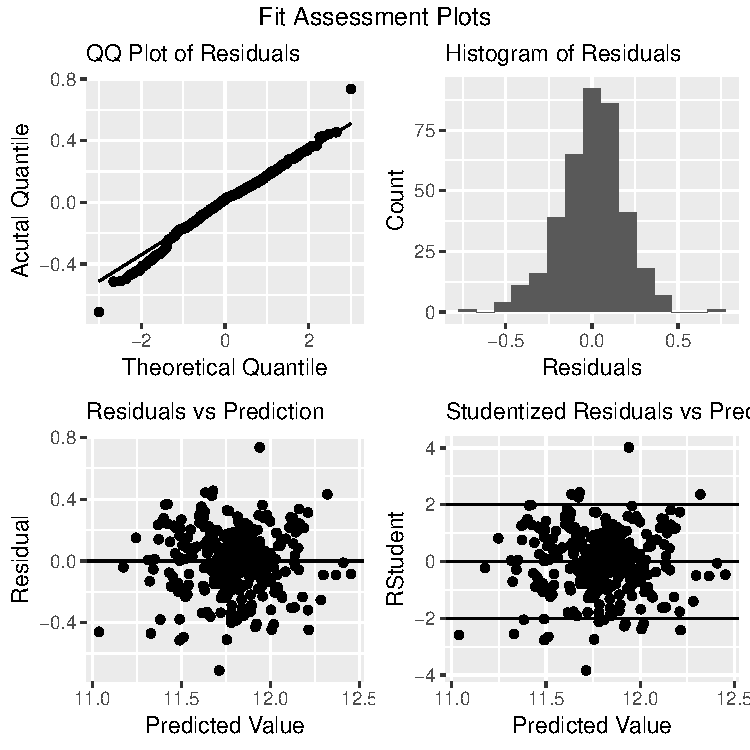
\includegraphics[width=0.45\linewidth]{HousePriceRegressionAnalysis_files/figure-latex/diag-plots-1} 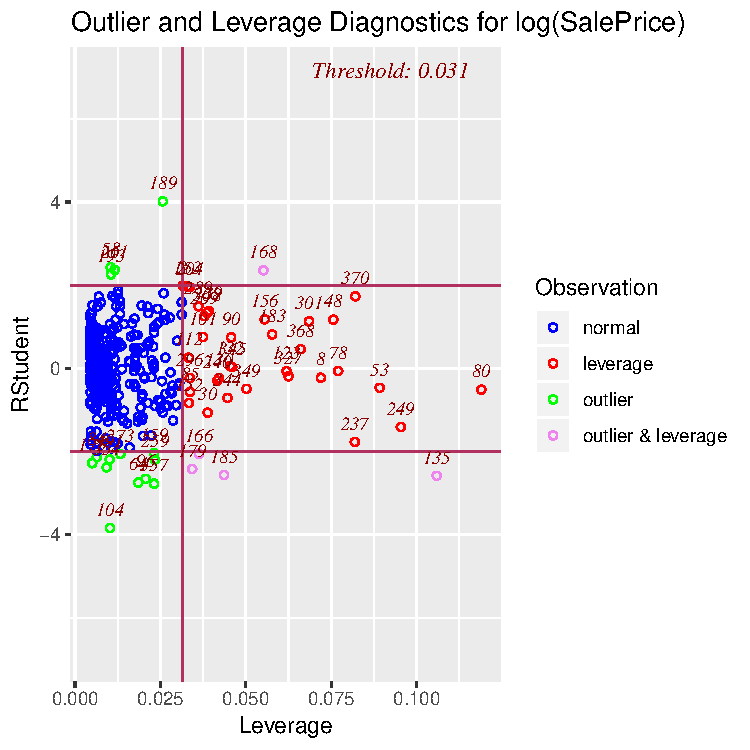
\includegraphics[width=0.45\linewidth]{HousePriceRegressionAnalysis_files/figure-latex/diag-plots-2} 

}

\caption{Diagnostic Plots}\label{fig:diag-plots}
\end{figure}

\hypertarget{comparing-competing-models}{%
\subsection{Comparing Competing
Models}\label{comparing-competing-models}}

The two models were trained and validated on the training dataset using
10-fold cross validation. The table below summerizes the performance of
the models with RMSE, adjusted \(R^2\), and PRESS. These results show
that the full model is an improvement over the reduced model, which is
consistent with the result of the ESS test.

\begin{table}[H]
\centering
\begin{tabular}{lrrr}
\toprule
Model & RMSE & CV.Press & Adjused.R.Squared\\
\midrule
Full Model & 0.1910566 & 12.51675 & 0.5084024\\
Reduced Model & 0.1988473 & 13.55835 & 0.4750767\\
\bottomrule
\end{tabular}
\end{table}

\hypertarget{parameters}{%
\subsection{Parameters}\label{parameters}}

The following table summerizes the parameter estimates for the full
model.

\begin{table}[H]
\centering
\begin{tabular}{lrrr}
\toprule
Parameter & Estimate & CI.Lower & CI.Upper\\
\midrule
Intercept & 11.0254845 & 10.8861855 & 11.1647836\\
GrLivArea & 0.0005387 & 0.0004324 & 11.1647836\\
Neighborhood\_BrkSide & -0.2338906 & -0.4468114 & -0.0209698\\
Neighborhood\_NAmes & 0.4178562 & 0.2558923 & 0.5798200\\
GrLivArea:Neighborhood\_BrkSide & 0.0001996 & 0.0000336 & 0.0003656\\
GrLivArea:Neighborhood\_NAmes & -0.0002145 & -0.0003366 & -0.0000924\\
\bottomrule
\end{tabular}
\end{table}

Where \texttt{Intercept} is \(\beta_0\), \texttt{GrLivArea} is
\(\beta_1\), \texttt{Neighborhood\_BrkSide} is \(\beta_2\),
\texttt{Neighborhood\_NAmes} is \(\beta_3\),
\texttt{GrLivArea:Neighborhood\_BrkSide} is \(\beta_4\), and
\texttt{GrLivArea:Neighborhood\_NAmes} is \(\beta_5\)

\hypertarget{model-interpretation}{%
\subsection{Model Interpretation}\label{model-interpretation}}

We estimate that for increase in 100 sq. ft., there is associated
multiplicative increase in median price of

\begin{itemize}
\tightlist
\item
  1.055 for the Edwards neighborhood with a 95\% confidence interval of
  {[}1.044 , 1.066{]}
\item
  1.033 for the Northwest Ames neighorhood with a 95\% confidence
  interval of {[}1.026 , 1.040{]}
\item
  1.077 for the Brookside neighorhood with a 95\% confidence interval of
  {[}1.063 , 1.090{]}
\end{itemize}

Since the sampling procedure is not known and this is an observational
study, the results only apply to this data.

\hypertarget{conclusion}{%
\subsection{Conclusion}\label{conclusion}}

In response to the analysis commissioned by Century 21, the log
transform of property sale price was modeled as a linear response to the
property living room area for residential properties in Ames, IA. It was
determined that it was necessary to include interaction terms to allow
for the influence of neighborhood on sale price. Based on the model,
there is strong evidence of an associated multiplicative increase in
median sale price for an increase in living room area (p-vlue
\textless{} 0.0001, overall F-test).

\hypertarget{analysis-question-ii}{%
\section{Analysis Question II}\label{analysis-question-ii}}

\hypertarget{question-of-interest-1}{%
\subsection{Question of Interest}\label{question-of-interest-1}}

Century 21 has commissioned a second analysis using the same data set,
expanded to include as many of the 80 total features, plus the index
split, as required to determine the sale price of residential properties
across all neighborhoods of Ames, Iowa, beyond only the three - Edwards,
Northwest Ames, and Brookside - previously commissioned for analysis.

\hypertarget{modeling-1}{%
\subsection{Modeling}\label{modeling-1}}

Restatement of Problem

Through analyzing our variable selection and cross-validation processes
- along with our nascant domain knowledge of residential real estate -
we ultimately arrived at a multiple linear regression model featuring 11
linear predictor variables and three interaction terms. Specifically,
our variable selection process included direct analysis of a correlation
plot and a correlation matrix as well as performing forward selection,
backward elimination, and stepwise regression. Because many variables
contained zeroes that were significant to the factor (for example,
bathrooms), we elected to perform logarithmic transformation only to
variable \texttt{LotArea}, representative of the area of the real estate
lot.

In addition to the transformation of \texttt{LotArea}, we imputed NA
values for 19 variables using a combination of the Data Dictionary
provided by Century 21 as well as our domain knowledge.

Type of selection

Forward Selection

Forward selection is a variable selection methodology that begins with a
constant mean and adds explanatory variables one-by-one until no further
additonal predictor variables significantly improve the model's fit.
This employess the ``F-to-enter'' method from the extra-sum-of-squares
F-statistic. This was the first method we employed. For this process, we
provided the test a starting model with no predictor variables and a
model from which terms can be selected, which included all predictor
variables available. The process worked forward with selecting one
parameter. The suggested model is output below.

\begin{Shaded}
\begin{Highlighting}[]
\CommentTok{# Initial Model - Forward Selection}
\NormalTok{model2.forward.Start <-}\StringTok{ }\KeywordTok{lm}\NormalTok{(}\KeywordTok{log}\NormalTok{(SalePrice)}\OperatorTok{~}\DecValTok{1}\NormalTok{,}\DataTypeTok{data =}\NormalTok{ train2)}

\CommentTok{# All Variables Model - Forward Selection}
\NormalTok{model2.Allvar <-}\StringTok{ }\KeywordTok{lm}\NormalTok{(}\KeywordTok{log}\NormalTok{(SalePrice) }\OperatorTok{~}\StringTok{ }\NormalTok{Id }\OperatorTok{+}\StringTok{ }\NormalTok{MSSubClass }\OperatorTok{+}\StringTok{ }\NormalTok{MSZoning }\OperatorTok{+}\StringTok{ }\NormalTok{LotFrontage }\OperatorTok{+}\StringTok{ }\NormalTok{LotArea }\OperatorTok{+}\StringTok{ }\NormalTok{Street }\OperatorTok{+}\StringTok{ }
\StringTok{                      }\NormalTok{Alley }\OperatorTok{+}\StringTok{ }\NormalTok{LotShape }\OperatorTok{+}\StringTok{ }\NormalTok{LandContour }\OperatorTok{+}\StringTok{ }\NormalTok{Utilities }\OperatorTok{+}\StringTok{ }\NormalTok{LotConfig }\OperatorTok{+}\StringTok{ }\NormalTok{LandSlope }\OperatorTok{+}
\StringTok{                      }\NormalTok{Neighborhood }\OperatorTok{+}\StringTok{ }\NormalTok{Condition1 }\OperatorTok{+}\StringTok{ }\NormalTok{Condition2 }\OperatorTok{+}\StringTok{ }\NormalTok{BldgType }\OperatorTok{+}\StringTok{ }\NormalTok{HouseStyle }\OperatorTok{+}\StringTok{ }\NormalTok{OverallQual }\OperatorTok{+}
\StringTok{                      }\NormalTok{OverallCond }\OperatorTok{+}\StringTok{ }\NormalTok{YearBuilt }\OperatorTok{+}\StringTok{ }\NormalTok{YearRemodAdd }\OperatorTok{+}\StringTok{ }\NormalTok{RoofStyle }\OperatorTok{+}\StringTok{ }\NormalTok{RoofMatl }\OperatorTok{+}\StringTok{ }\NormalTok{Exterior1st }\OperatorTok{+}
\StringTok{                      }\NormalTok{Exterior2nd }\OperatorTok{+}\StringTok{ }\NormalTok{MasVnrType }\OperatorTok{+}\StringTok{ }\NormalTok{MasVnrArea }\OperatorTok{+}\StringTok{ }\NormalTok{ExterQual }\OperatorTok{+}\StringTok{ }\NormalTok{ExterCond }\OperatorTok{+}\StringTok{ }\NormalTok{Foundation }\OperatorTok{+}
\StringTok{                      }\NormalTok{BsmtQual }\OperatorTok{+}\StringTok{ }\NormalTok{BsmtCond }\OperatorTok{+}\StringTok{ }\NormalTok{BsmtExposure }\OperatorTok{+}\StringTok{ }\NormalTok{BsmtFinType1 }\OperatorTok{+}\StringTok{ }\NormalTok{BsmtFinSF1 }\OperatorTok{+}\StringTok{ }\NormalTok{BsmtFinType2 }
                    \OperatorTok{+}\StringTok{ }\NormalTok{BsmtFinSF2 }\OperatorTok{+}\StringTok{ }\NormalTok{BsmtUnfSF }\OperatorTok{+}\StringTok{ }\NormalTok{TotalBsmtSF }\OperatorTok{+}\StringTok{ }\NormalTok{Heating }\OperatorTok{+}\StringTok{ }\NormalTok{HeatingQC }\OperatorTok{+}\StringTok{ }\NormalTok{CentralAir }\OperatorTok{+}\StringTok{ }
\StringTok{                      }\NormalTok{Electrical }\OperatorTok{+}\StringTok{ `}\DataTypeTok{1stFlrSF}\StringTok{`} \OperatorTok{+}\StringTok{ `}\DataTypeTok{2ndFlrSF}\StringTok{`} \OperatorTok{+}\StringTok{ }\NormalTok{LowQualFinSF }\OperatorTok{+}\StringTok{ }\NormalTok{GrLivArea }\OperatorTok{+}\StringTok{ }\NormalTok{BsmtFullBath}
                    \OperatorTok{+}\StringTok{ }\NormalTok{BsmtHalfBath }\OperatorTok{+}\StringTok{ }\NormalTok{FullBath }\OperatorTok{+}\StringTok{ }\NormalTok{HalfBath }\OperatorTok{+}\StringTok{ }\NormalTok{BedroomAbvGr }\OperatorTok{+}\StringTok{ }\NormalTok{KitchenAbvGr }\OperatorTok{+}\StringTok{ }\NormalTok{KitchenQual}
                    \OperatorTok{+}\StringTok{ }\NormalTok{TotRmsAbvGrd }\OperatorTok{+}\StringTok{ }\NormalTok{Functional }\OperatorTok{+}\StringTok{ }\NormalTok{Fireplaces }\OperatorTok{+}\StringTok{ }\NormalTok{FireplaceQu }\OperatorTok{+}\StringTok{ }\NormalTok{GarageType }\OperatorTok{+}
\StringTok{                      }\NormalTok{GarageYrBlt }\OperatorTok{+}\StringTok{ }\NormalTok{GarageFinish }\OperatorTok{+}\StringTok{ }\NormalTok{GarageCars }\OperatorTok{+}\StringTok{ }\NormalTok{GarageArea }\OperatorTok{+}\StringTok{ }\NormalTok{GarageQual }\OperatorTok{+}\StringTok{ }\NormalTok{GarageCond}
                    \OperatorTok{+}\StringTok{ }\NormalTok{PavedDrive }\OperatorTok{+}\StringTok{ }\NormalTok{WoodDeckSF }\OperatorTok{+}\StringTok{ }\NormalTok{OpenPorchSF }\OperatorTok{+}\StringTok{ }\NormalTok{EnclosedPorch }\OperatorTok{+}\StringTok{ `}\DataTypeTok{3SsnPorch}\StringTok{`} \OperatorTok{+}
\StringTok{                      }\NormalTok{ScreenPorch }\OperatorTok{+}\StringTok{ }\NormalTok{PoolArea }\OperatorTok{+}\StringTok{ }\NormalTok{PoolQC }\OperatorTok{+}\StringTok{ }\NormalTok{Fence }\OperatorTok{+}\StringTok{ }\NormalTok{MiscFeature }\OperatorTok{+}\StringTok{ }\NormalTok{MiscVal }\OperatorTok{+}\StringTok{ }\NormalTok{MoSold }\OperatorTok{+}
\StringTok{                      }\NormalTok{YrSold }\OperatorTok{+}\StringTok{ }\NormalTok{SaleType }\OperatorTok{+}\StringTok{ }\NormalTok{SaleCondition, }\DataTypeTok{data =}\NormalTok{ train2}
\NormalTok{                    )}

\NormalTok{model2.Forward <-}\StringTok{ }\KeywordTok{stepAIC}\NormalTok{(model2.forward.Start, }\DataTypeTok{direction =} \StringTok{"forward"}\NormalTok{, }\DataTypeTok{trace =}\NormalTok{ F, }\DataTypeTok{scope =} \KeywordTok{formula}\NormalTok{(model2.Allvar))}

\KeywordTok{summary}\NormalTok{(model2.Forward)}
\end{Highlighting}
\end{Shaded}

\begin{verbatim}
## 
## Call:
## lm(formula = log(SalePrice) ~ OverallQual + Neighborhood + GrLivArea + 
##     BsmtFinType1 + GarageCars + OverallCond + RoofMatl + TotalBsmtSF + 
##     YearBuilt + LotArea + Condition2 + MSZoning + BsmtUnfSF + 
##     SaleCondition + Functional + CentralAir + Condition1 + KitchenQual + 
##     Fireplaces + Exterior1st + Heating + ScreenPorch + YearRemodAdd + 
##     BsmtQual + PoolQC + Foundation + KitchenAbvGr + SaleType + 
##     GarageArea + HeatingQC + BsmtExposure + EnclosedPorch + WoodDeckSF + 
##     LotConfig + Street + BsmtFullBath + PoolArea + LandSlope + 
##     GarageCond + HalfBath + FullBath + TotRmsAbvGrd + `3SsnPorch` + 
##     ExterCond + GarageQual + GarageYrBlt + Utilities, data = train2)
## 
## Residuals:
##      Min       1Q   Median       3Q      Max 
## -0.72243 -0.04585  0.00175  0.05406  0.72243 
## 
## Coefficients: (2 not defined because of singularities)
##                        Estimate Std. Error t value Pr(>|t|)    
## (Intercept)           1.156e+00  9.003e-01   1.284 0.199342    
## OverallQual           4.534e-02  4.267e-03  10.625  < 2e-16 ***
## NeighborhoodBlueste  -1.828e-02  8.177e-02  -0.224 0.823149    
## NeighborhoodBrDale   -6.383e-02  4.388e-02  -1.455 0.146044    
## NeighborhoodBrkSide   1.077e-02  3.669e-02   0.294 0.769178    
## NeighborhoodClearCr  -1.217e-02  3.774e-02  -0.322 0.747241    
## NeighborhoodCollgCr  -4.672e-02  2.923e-02  -1.599 0.110164    
## NeighborhoodCrawfor   8.022e-02  3.486e-02   2.301 0.021539 *  
## NeighborhoodEdwards  -1.037e-01  3.226e-02  -3.215 0.001337 ** 
## NeighborhoodGilbert  -4.801e-02  3.121e-02  -1.538 0.124258    
## NeighborhoodIDOTRR   -4.462e-02  4.267e-02  -1.046 0.295897    
## NeighborhoodMeadowV  -1.632e-01  4.637e-02  -3.520 0.000446 ***
## NeighborhoodMitchel  -9.451e-02  3.349e-02  -2.822 0.004844 ** 
## NeighborhoodNAmes    -5.862e-02  3.138e-02  -1.868 0.061937 .  
## NeighborhoodNoRidge   1.077e-02  3.408e-02   0.316 0.752018    
## NeighborhoodNPkVill  -1.274e-02  4.704e-02  -0.271 0.786616    
## NeighborhoodNridgHt   3.664e-02  3.044e-02   1.204 0.228936    
## NeighborhoodNWAmes   -6.179e-02  3.293e-02  -1.877 0.060793 .  
## NeighborhoodOldTown  -5.731e-02  3.739e-02  -1.533 0.125636    
## NeighborhoodSawyer   -5.556e-02  3.313e-02  -1.677 0.093742 .  
## NeighborhoodSawyerW  -4.766e-02  3.233e-02  -1.474 0.140677    
## NeighborhoodSomerst   8.423e-03  3.675e-02   0.229 0.818755    
## NeighborhoodStoneBr   8.120e-02  3.506e-02   2.316 0.020696 *  
## NeighborhoodSWISU    -2.141e-02  3.892e-02  -0.550 0.582229    
## NeighborhoodTimber   -3.348e-02  3.364e-02  -0.995 0.319801    
## NeighborhoodVeenker  -9.409e-03  4.540e-02  -0.207 0.835861    
## GrLivArea             2.140e-04  1.608e-05  13.311  < 2e-16 ***
## BsmtFinType1ALQ      -5.270e-02  1.096e-01  -0.481 0.630830    
## BsmtFinType1BLQ      -6.157e-02  1.096e-01  -0.562 0.574543    
## BsmtFinType1GLQ      -4.235e-02  1.098e-01  -0.386 0.699892    
## BsmtFinType1LwQ      -7.859e-02  1.100e-01  -0.715 0.474988    
## BsmtFinType1Rec      -6.949e-02  1.097e-01  -0.634 0.526454    
## BsmtFinType1Unf      -7.221e-02  1.092e-01  -0.661 0.508643    
## GarageCars            2.050e-02  9.942e-03   2.062 0.039387 *  
## OverallCond           3.719e-02  3.726e-03   9.982  < 2e-16 ***
## RoofMatlCompShg       2.517e+00  1.986e-01  12.671  < 2e-16 ***
## RoofMatlMembran       2.730e+00  2.311e-01  11.815  < 2e-16 ***
## RoofMatlMetal         2.592e+00  2.307e-01  11.236  < 2e-16 ***
## RoofMatlRoll          2.562e+00  2.283e-01  11.223  < 2e-16 ***
## RoofMatlTar&Grv       2.496e+00  2.042e-01  12.228  < 2e-16 ***
## RoofMatlWdShake       2.542e+00  2.055e-01  12.371  < 2e-16 ***
## RoofMatlWdShngl       2.545e+00  2.023e-01  12.585  < 2e-16 ***
## TotalBsmtSF           1.477e-04  1.523e-05   9.694  < 2e-16 ***
## YearBuilt             2.039e-03  3.156e-04   6.458 1.49e-10 ***
## LotArea               8.909e-02  1.000e-02   8.908  < 2e-16 ***
## Condition2Feedr       7.729e-02  9.623e-02   0.803 0.422021    
## Condition2Norm        4.081e-02  8.255e-02   0.494 0.621127    
## Condition2PosA        2.971e-01  1.541e-01   1.929 0.053972 .  
## Condition2PosN       -8.390e-01  1.171e-01  -7.163 1.31e-12 ***
## Condition2RRAe       -1.399e-01  1.347e-01  -1.039 0.299064    
## Condition2RRAn       -8.032e-02  1.343e-01  -0.598 0.549881    
## Condition2RRNn       -1.358e-02  1.146e-01  -0.119 0.905654    
## MSZoningFV            4.209e-01  5.158e-02   8.160 7.82e-16 ***
## MSZoningRH            4.154e-01  5.135e-02   8.089 1.37e-15 ***
## MSZoningRL            4.019e-01  4.368e-02   9.203  < 2e-16 ***
## MSZoningRM            3.711e-01  4.088e-02   9.078  < 2e-16 ***
## BsmtUnfSF            -5.325e-05  1.291e-05  -4.123 3.97e-05 ***
## SaleConditionAdjLand  1.243e-01  5.779e-02   2.150 0.031734 *  
## SaleConditionAlloca   4.331e-02  3.720e-02   1.164 0.244486    
## SaleConditionFamily   1.532e-02  2.691e-02   0.569 0.569387    
## SaleConditionNormal   7.074e-02  1.268e-02   5.580 2.93e-08 ***
## SaleConditionPartial -5.574e-02  6.543e-02  -0.852 0.394473    
## FunctionalMaj2       -2.367e-01  5.882e-02  -4.024 6.05e-05 ***
## FunctionalMin1        4.359e-02  3.581e-02   1.217 0.223685    
## FunctionalMin2        4.480e-02  3.535e-02   1.267 0.205325    
## FunctionalMod        -4.948e-02  4.315e-02  -1.147 0.251792    
## FunctionalSev        -2.619e-01  1.175e-01  -2.229 0.025995 *  
## FunctionalTyp         7.740e-02  3.052e-02   2.536 0.011340 *  
## CentralAirY           6.380e-02  1.591e-02   4.011 6.38e-05 ***
## Condition1Feedr       4.539e-02  2.158e-02   2.103 0.035674 *  
## Condition1Norm        8.223e-02  1.785e-02   4.608 4.47e-06 ***
## Condition1PosA        4.391e-02  4.284e-02   1.025 0.305519    
## Condition1PosN        8.746e-02  3.193e-02   2.739 0.006243 ** 
## Condition1RRAe       -4.912e-02  3.987e-02  -1.232 0.218225    
## Condition1RRAn        4.088e-02  2.981e-02   1.371 0.170510    
## Condition1RRNe        2.394e-02  7.837e-02   0.305 0.760077    
## Condition1RRNn        8.546e-02  5.481e-02   1.559 0.119156    
## KitchenQualFa        -5.620e-02  2.582e-02  -2.177 0.029690 *  
## KitchenQualGd        -5.437e-02  1.439e-02  -3.779 0.000165 ***
## KitchenQualTA        -5.434e-02  1.644e-02  -3.306 0.000973 ***
## Fireplaces            2.164e-02  5.782e-03   3.743 0.000190 ***
## Exterior1stAsphShn    3.372e-02  1.122e-01   0.301 0.763724    
## Exterior1stBrkComm   -1.500e-01  8.675e-02  -1.729 0.084059 .  
## Exterior1stBrkFace    8.658e-02  3.098e-02   2.795 0.005271 ** 
## Exterior1stCBlock    -2.912e-02  1.110e-01  -0.262 0.793151    
## Exterior1stCemntBd    3.653e-02  3.249e-02   1.124 0.261090    
## Exterior1stHdBoard    4.786e-03  2.832e-02   0.169 0.865811    
## Exterior1stImStucc    1.779e-03  1.091e-01   0.016 0.986992    
## Exterior1stMetalSd    3.256e-02  2.735e-02   1.190 0.234082    
## Exterior1stPlywood    1.015e-02  2.972e-02   0.342 0.732706    
## Exterior1stStone     -1.733e-02  8.554e-02  -0.203 0.839534    
## Exterior1stStucco     4.550e-02  3.497e-02   1.301 0.193459    
## Exterior1stVinylSd    2.773e-02  2.759e-02   1.005 0.315019    
## Exterior1stWd Sdng    2.130e-03  2.740e-02   0.078 0.938050    
## Exterior1stWdShing    1.068e-02  3.421e-02   0.312 0.754861    
## HeatingGasA           1.306e-01  1.138e-01   1.147 0.251487    
## HeatingGasW           2.122e-01  1.171e-01   1.812 0.070189 .  
## HeatingGrav          -2.092e-02  1.230e-01  -0.170 0.864987    
## HeatingOthW           1.733e-01  1.388e-01   1.248 0.212090    
## HeatingWall           1.888e-01  1.291e-01   1.462 0.143934    
## ScreenPorch           2.478e-04  5.473e-05   4.527 6.52e-06 ***
## YearRemodAdd          7.768e-04  2.340e-04   3.319 0.000929 ***
## BsmtQualEx            5.017e-02  1.753e-02   2.862 0.004274 ** 
## BsmtQualFa            1.652e-02  2.069e-02   0.799 0.424585    
## BsmtQualGd            7.765e-03  1.067e-02   0.728 0.466730    
## BsmtQualTA                   NA         NA      NA       NA    
## PoolQCFa             -1.186e-01  1.182e-01  -1.003 0.316025    
## PoolQCGd              8.872e-02  1.413e-01   0.628 0.530171    
## PoolQCNone            9.036e-01  4.108e-01   2.200 0.027989 *  
## FoundationCBlock      1.872e-02  1.369e-02   1.367 0.171852    
## FoundationPConc       3.742e-02  1.498e-02   2.497 0.012637 *  
## FoundationSlab       -2.317e-03  4.301e-02  -0.054 0.957042    
## FoundationStone       1.037e-01  4.668e-02   2.222 0.026426 *  
## FoundationWood       -1.163e-01  6.419e-02  -1.812 0.070191 .  
## KitchenAbvGr         -5.693e-02  1.724e-02  -3.302 0.000985 ***
## SaleTypeCon           4.102e-02  7.839e-02   0.523 0.600868    
## SaleTypeConLD         1.264e-01  4.199e-02   3.011 0.002654 ** 
## SaleTypeConLI        -3.210e-02  5.071e-02  -0.633 0.526833    
## SaleTypeConLw         1.291e-02  5.215e-02   0.248 0.804473    
## SaleTypeCWD           5.621e-02  5.681e-02   0.989 0.322668    
## SaleTypeNew           1.558e-01  6.784e-02   2.297 0.021787 *  
## SaleTypeOth           5.535e-02  6.437e-02   0.860 0.390039    
## SaleTypeWD           -1.896e-02  1.830e-02  -1.036 0.300280    
## GarageArea            1.014e-04  3.410e-05   2.974 0.002993 ** 
## HeatingQCFa          -3.036e-02  2.005e-02  -1.514 0.130261    
## HeatingQCGd          -2.151e-02  9.049e-03  -2.377 0.017589 *  
## HeatingQCPo          -4.834e-02  1.141e-01  -0.424 0.671941    
## HeatingQCTA          -3.692e-02  8.979e-03  -4.112 4.18e-05 ***
## BsmtExposureAv        6.546e-02  1.039e-01   0.630 0.528649    
## BsmtExposureGd        1.043e-01  1.043e-01   1.000 0.317348    
## BsmtExposureMn        6.107e-02  1.041e-01   0.586 0.557645    
## BsmtExposureNo        5.632e-02  1.037e-01   0.543 0.587153    
## EnclosedPorch         1.198e-04  5.360e-05   2.236 0.025549 *  
## WoodDeckSF            6.805e-05  2.572e-05   2.646 0.008240 ** 
## LotConfigCulDSac      1.137e-02  1.372e-02   0.829 0.407341    
## LotConfigFR2         -4.420e-02  1.748e-02  -2.529 0.011562 *  
## LotConfigFR3         -9.740e-02  5.591e-02  -1.742 0.081705 .  
## LotConfigInside      -1.580e-02  7.682e-03  -2.057 0.039888 *  
## StreetPave            1.106e-01  4.844e-02   2.284 0.022545 *  
## BsmtFullBath          2.162e-02  8.120e-03   2.663 0.007845 ** 
## PoolArea              1.679e-03  7.539e-04   2.228 0.026072 *  
## LandSlopeMod          1.755e-02  1.515e-02   1.158 0.247052    
## LandSlopeSev         -7.623e-02  3.792e-02  -2.011 0.044573 *  
## GarageCondFa          1.826e-01  1.443e-01   1.265 0.205988    
## GarageCondGd          2.152e-01  1.480e-01   1.454 0.146055    
## GarageCondNone       -7.047e-02  7.739e-02  -0.911 0.362683    
## GarageCondPo          3.425e-01  1.551e-01   2.208 0.027399 *  
## GarageCondTA          2.231e-01  1.426e-01   1.564 0.117963    
## HalfBath              2.271e-02  8.330e-03   2.726 0.006496 ** 
## FullBath              1.935e-02  9.364e-03   2.066 0.039000 *  
## TotRmsAbvGrd          6.493e-03  3.671e-03   1.769 0.077166 .  
## `3SsnPorch`           1.477e-04  9.884e-05   1.494 0.135342    
## ExterCondFa          -6.253e-02  7.903e-02  -0.791 0.429005    
## ExterCondGd          -5.048e-02  7.515e-02  -0.672 0.501919    
## ExterCondPo          -6.132e-02  1.365e-01  -0.449 0.653358    
## ExterCondTA          -2.644e-02  7.504e-02  -0.352 0.724688    
## GarageQualFa         -3.025e-01  1.229e-01  -2.461 0.013967 *  
## GarageQualGd         -2.405e-01  1.255e-01  -1.916 0.055587 .  
## GarageQualNone               NA         NA      NA       NA    
## GarageQualPo         -3.614e-01  1.519e-01  -2.379 0.017502 *  
## GarageQualTA         -2.645e-01  1.212e-01  -2.183 0.029243 *  
## GarageYrBlt          -4.060e-04  2.587e-04  -1.569 0.116882    
## UtilitiesNoSeWa      -1.608e-01  1.094e-01  -1.471 0.141567    
## ---
## Signif. codes:  0 '***' 0.001 '**' 0.01 '*' 0.05 '.' 0.1 ' ' 1
## 
## Residual standard error: 0.1028 on 1299 degrees of freedom
## Multiple R-squared:  0.941,  Adjusted R-squared:  0.9337 
## F-statistic: 129.5 on 160 and 1299 DF,  p-value: < 2.2e-16
\end{verbatim}

\begin{Shaded}
\begin{Highlighting}[]
\NormalTok{model2.Forward}\OperatorTok{$}\NormalTok{anova}
\end{Highlighting}
\end{Shaded}

\begin{verbatim}
## Stepwise Model Path 
## Analysis of Deviance Table
## 
## Initial Model:
## log(SalePrice) ~ 1
## 
## Final Model:
## log(SalePrice) ~ OverallQual + Neighborhood + GrLivArea + BsmtFinType1 + 
##     GarageCars + OverallCond + RoofMatl + TotalBsmtSF + YearBuilt + 
##     LotArea + Condition2 + MSZoning + BsmtUnfSF + SaleCondition + 
##     Functional + CentralAir + Condition1 + KitchenQual + Fireplaces + 
##     Exterior1st + Heating + ScreenPorch + YearRemodAdd + BsmtQual + 
##     PoolQC + Foundation + KitchenAbvGr + SaleType + GarageArea + 
##     HeatingQC + BsmtExposure + EnclosedPorch + WoodDeckSF + LotConfig + 
##     Street + BsmtFullBath + PoolArea + LandSlope + GarageCond + 
##     HalfBath + FullBath + TotRmsAbvGrd + `3SsnPorch` + ExterCond + 
##     GarageQual + GarageYrBlt + Utilities
## 
## 
##               Step Df     Deviance Resid. Df Resid. Dev       AIC
## 1                                       1459  232.80066 -2678.573
## 2    + OverallQual  1 155.46203888      1458   77.33862 -4285.477
## 3   + Neighborhood 24  20.64653490      1434   56.69209 -4690.893
## 4      + GrLivArea  1  14.83069906      1433   41.86139 -5131.669
## 5   + BsmtFinType1  6   4.03327119      1427   37.82811 -5267.583
## 6     + GarageCars  1   3.26135246      1426   34.56676 -5397.217
## 7    + OverallCond  1   2.68083808      1425   31.88592 -5513.079
## 8       + RoofMatl  7   2.27800530      1418   29.60792 -5607.299
## 9    + TotalBsmtSF  1   2.90424457      1417   26.70367 -5756.030
## 10     + YearBuilt  1   1.54304245      1416   25.16063 -5840.930
## 11       + LotArea  1   1.79077988      1415   23.36985 -5946.728
## 12    + Condition2  7   1.46488205      1408   21.90497 -6027.238
## 13      + MSZoning  4   0.95147479      1404   20.95350 -6084.074
## 14     + BsmtUnfSF  1   0.67072280      1403   20.28277 -6129.573
## 15 + SaleCondition  5   0.84137276      1398   19.44140 -6181.429
## 16    + Functional  6   0.73550628      1392   18.70589 -6225.735
## 17    + CentralAir  1   0.46022681      1391   18.24567 -6260.106
## 18    + Condition1  8   0.53482973      1383   17.71084 -6287.542
## 19   + KitchenQual  3   0.37132218      1380   17.33951 -6312.477
## 20    + Fireplaces  1   0.26880260      1379   17.07071 -6333.288
## 21   + Exterior1st 14   0.54350008      1365   16.52721 -6352.528
## 22       + Heating  5   0.27522498      1360   16.25199 -6367.046
## 23   + ScreenPorch  1   0.15569020      1359   16.09630 -6379.100
## 24  + YearRemodAdd  1   0.15411911      1358   15.94218 -6391.146
## 25      + BsmtQual  3   0.18403447      1355   15.75814 -6402.098
## 26        + PoolQC  3   0.15215182      1352   15.60599 -6410.264
## 27    + Foundation  5   0.18551221      1347   15.42048 -6417.723
## 28  + KitchenAbvGr  1   0.10252599      1346   15.31795 -6425.463
## 29      + SaleType  8   0.24240360      1338   15.07555 -6432.752
## 30    + GarageArea  1   0.09371674      1337   14.98183 -6439.856
## 31     + HeatingQC  4   0.15007917      1333   14.83175 -6446.555
## 32  + BsmtExposure  4   0.13705578      1329   14.69470 -6452.109
## 33 + EnclosedPorch  1   0.06780557      1328   14.62689 -6456.862
## 34    + WoodDeckSF  1   0.06736739      1327   14.55953 -6461.602
## 35     + LotConfig  4   0.11722845      1323   14.44230 -6465.405
## 36        + Street  1   0.05761598      1322   14.38468 -6469.241
## 37  + BsmtFullBath  1   0.05359166      1321   14.33109 -6472.690
## 38      + PoolArea  1   0.04846687      1320   14.28262 -6475.636
## 39     + LandSlope  2   0.06762462      1318   14.21500 -6478.565
## 40    + GarageCond  5   0.12893599      1313   14.08606 -6481.869
## 41      + HalfBath  1   0.04484913      1312   14.04121 -6484.525
## 42      + FullBath  1   0.04414227      1311   13.99707 -6487.122
## 43  + TotRmsAbvGrd  1   0.02713930      1310   13.96993 -6487.955
## 44   + `3SsnPorch`  1   0.02428567      1309   13.94565 -6488.496
## 45     + ExterCond  4   0.07902859      1305   13.86662 -6488.793
## 46    + GarageQual  4   0.08008028      1301   13.78654 -6489.249
## 47   + GarageYrBlt  1   0.02479572      1300   13.76174 -6489.877
## 48     + Utilities  1   0.02288193      1299   13.73886 -6490.307
\end{verbatim}

\begin{Shaded}
\begin{Highlighting}[]
\NormalTok{final.Forward.Model <-}\StringTok{ }\KeywordTok{lm}\NormalTok{(}\KeywordTok{log}\NormalTok{(SalePrice) }\OperatorTok{~}\StringTok{ }\NormalTok{OverallQual }\OperatorTok{+}\StringTok{ }\NormalTok{Neighborhood }\OperatorTok{+}\StringTok{ }\NormalTok{GrLivArea }\OperatorTok{+}\StringTok{ }\NormalTok{BsmtFinType1 }\OperatorTok{+}\StringTok{ }
\StringTok{                  }\NormalTok{GarageCars }\OperatorTok{+}\StringTok{ }\NormalTok{OverallCond }\OperatorTok{+}\StringTok{ }\NormalTok{RoofMatl }\OperatorTok{+}\StringTok{ }\NormalTok{TotalBsmtSF }\OperatorTok{+}\StringTok{ }\NormalTok{YearBuilt }\OperatorTok{+}\StringTok{ }
\StringTok{                  }\NormalTok{LotArea }\OperatorTok{+}\StringTok{ }\NormalTok{Condition2 }\OperatorTok{+}\StringTok{ }\NormalTok{MSZoning }\OperatorTok{+}\StringTok{ }\NormalTok{BsmtUnfSF }\OperatorTok{+}\StringTok{ }\NormalTok{SaleCondition }\OperatorTok{+}\StringTok{ }
\StringTok{                  }\NormalTok{Functional }\OperatorTok{+}\StringTok{ }\NormalTok{CentralAir }\OperatorTok{+}\StringTok{ }\NormalTok{Condition1 }\OperatorTok{+}\StringTok{ }\NormalTok{KitchenQual }\OperatorTok{+}\StringTok{ }\NormalTok{Fireplaces }\OperatorTok{+}\StringTok{ }
\StringTok{                  }\NormalTok{Exterior1st }\OperatorTok{+}\StringTok{ }\NormalTok{Heating }\OperatorTok{+}\StringTok{ }\NormalTok{ScreenPorch }\OperatorTok{+}\StringTok{ }\NormalTok{YearRemodAdd }\OperatorTok{+}\StringTok{ }\NormalTok{BsmtQual }\OperatorTok{+}\StringTok{ }
\StringTok{                  }\NormalTok{PoolQC }\OperatorTok{+}\StringTok{ }\NormalTok{Foundation }\OperatorTok{+}\StringTok{ }\NormalTok{KitchenAbvGr }\OperatorTok{+}\StringTok{ }\NormalTok{SaleType }\OperatorTok{+}\StringTok{ }\NormalTok{GarageArea }\OperatorTok{+}\StringTok{ }
\StringTok{                  }\NormalTok{HeatingQC }\OperatorTok{+}\StringTok{ }\NormalTok{BsmtExposure }\OperatorTok{+}\StringTok{ }\NormalTok{EnclosedPorch }\OperatorTok{+}\StringTok{ }\NormalTok{WoodDeckSF }\OperatorTok{+}\StringTok{ }\NormalTok{LotConfig }\OperatorTok{+}\StringTok{ }
\StringTok{                  }\NormalTok{Street }\OperatorTok{+}\StringTok{ }\NormalTok{BsmtFullBath }\OperatorTok{+}\StringTok{ }\NormalTok{PoolArea }\OperatorTok{+}\StringTok{ }\NormalTok{LandSlope }\OperatorTok{+}\StringTok{ }\NormalTok{GarageCond }\OperatorTok{+}\StringTok{ }
\StringTok{                  }\NormalTok{HalfBath }\OperatorTok{+}\StringTok{ }\NormalTok{FullBath }\OperatorTok{+}\StringTok{ }\NormalTok{TotRmsAbvGrd }\OperatorTok{+}\StringTok{ `}\DataTypeTok{3SsnPorch}\StringTok{`} \OperatorTok{+}\StringTok{ }\NormalTok{ExterCond }\OperatorTok{+}\StringTok{ }
\StringTok{                  }\NormalTok{GarageQual }\OperatorTok{+}\StringTok{ }\NormalTok{GarageYrBlt }\OperatorTok{+}\StringTok{ }\NormalTok{Utilities, }\DataTypeTok{data =}\NormalTok{ train2}
\NormalTok{                  )}
\end{Highlighting}
\end{Shaded}

Backward Elimination

Backward elimination is a variable selection methodology that begins
with all possible predictor variables and works backward, eliminating
variables using all possible combinations until only the best for the
fit are provided. This employess the ``F-to-remove'' method from the
extra-sum-of-squares F-statistic. For this process, we provided the test
a model with all available predictor variables from which insignificant
variables were eliminated. The output is as follows below.

\begin{verbatim}
## 
## Call:
## lm(formula = log(SalePrice) ~ MSZoning + LotArea + Street + LotConfig + 
##     LandSlope + Neighborhood + Condition1 + Condition2 + OverallQual + 
##     OverallCond + YearBuilt + YearRemodAdd + RoofMatl + Exterior1st + 
##     ExterCond + Foundation + BsmtQual + BsmtExposure + BsmtFinSF1 + 
##     BsmtFinSF2 + BsmtUnfSF + Heating + HeatingQC + CentralAir + 
##     `1stFlrSF` + `2ndFlrSF` + LowQualFinSF + BsmtFullBath + FullBath + 
##     HalfBath + KitchenAbvGr + KitchenQual + TotRmsAbvGrd + Functional + 
##     Fireplaces + GarageCars + GarageArea + GarageQual + GarageCond + 
##     WoodDeckSF + EnclosedPorch + `3SsnPorch` + ScreenPorch + 
##     PoolArea + PoolQC + SaleType + SaleCondition, data = train2)
## 
## Residuals:
##      Min       1Q   Median       3Q      Max 
## -0.73120 -0.04561  0.00172  0.05490  0.73120 
## 
## Coefficients: (1 not defined because of singularities)
##                        Estimate Std. Error t value Pr(>|t|)    
## (Intercept)           4.266e-01  8.405e-01   0.508 0.611822    
## MSZoningFV            4.232e-01  5.158e-02   8.205 5.48e-16 ***
## MSZoningRH            4.156e-01  5.135e-02   8.092 1.33e-15 ***
## MSZoningRL            4.046e-01  4.366e-02   9.267  < 2e-16 ***
## MSZoningRM            3.720e-01  4.087e-02   9.102  < 2e-16 ***
## LotArea               8.957e-02  9.910e-03   9.038  < 2e-16 ***
## StreetPave            1.092e-01  4.837e-02   2.257 0.024168 *  
## LotConfigCulDSac      8.514e-03  1.366e-02   0.623 0.533289    
## LotConfigFR2         -4.098e-02  1.747e-02  -2.346 0.019108 *  
## LotConfigFR3         -9.211e-02  5.588e-02  -1.648 0.099509 .  
## LotConfigInside      -1.436e-02  7.645e-03  -1.878 0.060599 .  
## LandSlopeMod          1.609e-02  1.517e-02   1.060 0.289200    
## LandSlopeSev         -7.893e-02  3.793e-02  -2.081 0.037631 *  
## NeighborhoodBlueste  -1.262e-02  8.181e-02  -0.154 0.877419    
## NeighborhoodBrDale   -6.156e-02  4.393e-02  -1.401 0.161392    
## NeighborhoodBrkSide   1.229e-02  3.675e-02   0.335 0.738051    
## NeighborhoodClearCr  -8.026e-03  3.819e-02  -0.210 0.833565    
## NeighborhoodCollgCr  -4.798e-02  2.940e-02  -1.632 0.102904    
## NeighborhoodCrawfor   8.246e-02  3.486e-02   2.366 0.018151 *  
## NeighborhoodEdwards  -1.052e-01  3.244e-02  -3.242 0.001218 ** 
## NeighborhoodGilbert  -5.301e-02  3.135e-02  -1.691 0.091071 .  
## NeighborhoodIDOTRR   -3.864e-02  4.270e-02  -0.905 0.365690    
## NeighborhoodMeadowV  -1.558e-01  4.615e-02  -3.376 0.000758 ***
## NeighborhoodMitchel  -9.347e-02  3.359e-02  -2.782 0.005472 ** 
## NeighborhoodNAmes    -5.696e-02  3.145e-02  -1.811 0.070346 .  
## NeighborhoodNoRidge   1.011e-02  3.435e-02   0.294 0.768597    
## NeighborhoodNPkVill  -3.641e-03  4.683e-02  -0.078 0.938041    
## NeighborhoodNridgHt   3.511e-02  3.064e-02   1.146 0.252054    
## NeighborhoodNWAmes   -5.784e-02  3.292e-02  -1.757 0.079192 .  
## NeighborhoodOldTown  -5.305e-02  3.751e-02  -1.414 0.157462    
## NeighborhoodSawyer   -5.567e-02  3.318e-02  -1.678 0.093665 .  
## NeighborhoodSawyerW  -4.701e-02  3.243e-02  -1.450 0.147364    
## NeighborhoodSomerst   7.367e-03  3.683e-02   0.200 0.841496    
## NeighborhoodStoneBr   8.119e-02  3.514e-02   2.311 0.021015 *  
## NeighborhoodSWISU    -1.314e-02  3.927e-02  -0.335 0.738011    
## NeighborhoodTimber   -4.081e-02  3.363e-02  -1.214 0.225115    
## NeighborhoodVeenker  -1.408e-02  4.534e-02  -0.311 0.756160    
## Condition1Feedr       4.537e-02  2.158e-02   2.103 0.035651 *  
## Condition1Norm        8.266e-02  1.781e-02   4.640 3.83e-06 ***
## Condition1PosA        4.460e-02  4.303e-02   1.036 0.300227    
## Condition1PosN        8.432e-02  3.194e-02   2.640 0.008387 ** 
## Condition1RRAe       -4.973e-02  3.993e-02  -1.245 0.213264    
## Condition1RRAn        3.845e-02  2.969e-02   1.295 0.195581    
## Condition1RRNe        2.909e-02  7.831e-02   0.371 0.710405    
## Condition1RRNn        8.423e-02  5.477e-02   1.538 0.124342    
## Condition2Feedr       6.606e-02  9.613e-02   0.687 0.492029    
## Condition2Norm        2.643e-02  8.243e-02   0.321 0.748548    
## Condition2PosA        2.720e-01  1.537e-01   1.769 0.077131 .  
## Condition2PosN       -8.582e-01  1.170e-01  -7.334 3.92e-13 ***
## Condition2RRAe       -1.247e-01  1.347e-01  -0.926 0.354563    
## Condition2RRAn       -9.775e-02  1.343e-01  -0.728 0.466739    
## Condition2RRNn       -2.677e-02  1.143e-01  -0.234 0.814942    
## OverallQual           4.580e-02  4.226e-03  10.838  < 2e-16 ***
## OverallCond           3.795e-02  3.678e-03  10.319  < 2e-16 ***
## YearBuilt             2.027e-03  3.084e-04   6.574 7.05e-11 ***
## YearRemodAdd          7.533e-04  2.328e-04   3.236 0.001242 ** 
## RoofMatlCompShg       2.588e+00  1.971e-01  13.133  < 2e-16 ***
## RoofMatlMembran       2.815e+00  2.313e-01  12.172  < 2e-16 ***
## RoofMatlMetal         2.664e+00  2.294e-01  11.611  < 2e-16 ***
## RoofMatlRoll          2.643e+00  2.256e-01  11.718  < 2e-16 ***
## RoofMatlTar&Grv       2.576e+00  2.029e-01  12.697  < 2e-16 ***
## RoofMatlWdShake       2.608e+00  2.047e-01  12.739  < 2e-16 ***
## RoofMatlWdShngl       2.619e+00  2.007e-01  13.049  < 2e-16 ***
## Exterior1stAsphShn    2.942e-02  1.129e-01   0.261 0.794465    
## Exterior1stBrkComm   -1.445e-01  8.688e-02  -1.664 0.096402 .  
## Exterior1stBrkFace    9.118e-02  3.097e-02   2.945 0.003292 ** 
## Exterior1stCBlock    -1.595e-02  1.107e-01  -0.144 0.885434    
## Exterior1stCemntBd    3.761e-02  3.241e-02   1.161 0.246001    
## Exterior1stHdBoard    8.831e-03  2.824e-02   0.313 0.754530    
## Exterior1stImStucc    1.300e-03  1.092e-01   0.012 0.990507    
## Exterior1stMetalSd    3.632e-02  2.737e-02   1.327 0.184723    
## Exterior1stPlywood    1.240e-02  2.968e-02   0.418 0.676177    
## Exterior1stStone     -2.733e-03  8.633e-02  -0.032 0.974753    
## Exterior1stStucco     4.735e-02  3.477e-02   1.362 0.173503    
## Exterior1stVinylSd    3.047e-02  2.761e-02   1.104 0.269907    
## Exterior1stWd Sdng    4.887e-03  2.736e-02   0.179 0.858277    
## Exterior1stWdShing    1.371e-02  3.417e-02   0.401 0.688369    
## ExterCondFa          -6.467e-02  7.898e-02  -0.819 0.413026    
## ExterCondGd          -5.206e-02  7.505e-02  -0.694 0.487999    
## ExterCondPo          -6.700e-02  1.369e-01  -0.489 0.624675    
## ExterCondTA          -2.915e-02  7.494e-02  -0.389 0.697347    
## FoundationCBlock      1.752e-02  1.366e-02   1.282 0.200095    
## FoundationPConc       3.701e-02  1.497e-02   2.472 0.013555 *  
## FoundationSlab       -2.874e-03  4.305e-02  -0.067 0.946783    
## FoundationStone       1.067e-01  4.661e-02   2.288 0.022287 *  
## FoundationWood       -1.198e-01  6.406e-02  -1.870 0.061658 .  
## BsmtQualEx           -2.908e-02  1.117e-01  -0.260 0.794559    
## BsmtQualFa           -6.214e-02  1.116e-01  -0.557 0.577654    
## BsmtQualGd           -6.800e-02  1.107e-01  -0.614 0.539034    
## BsmtQualTA           -7.552e-02  1.102e-01  -0.685 0.493427    
## BsmtExposureAv        7.904e-02  1.039e-01   0.760 0.447130    
## BsmtExposureGd        1.170e-01  1.044e-01   1.121 0.262442    
## BsmtExposureMn        7.427e-02  1.042e-01   0.713 0.476110    
## BsmtExposureNo        6.757e-02  1.038e-01   0.651 0.515072    
## BsmtFinSF1            1.557e-04  1.985e-05   7.845 9.00e-15 ***
## BsmtFinSF2            1.206e-04  2.533e-05   4.763 2.12e-06 ***
## BsmtUnfSF             8.636e-05  1.877e-05   4.602 4.60e-06 ***
## HeatingGasA           1.307e-01  1.140e-01   1.147 0.251499    
## HeatingGasW           2.143e-01  1.171e-01   1.830 0.067509 .  
## HeatingGrav          -2.660e-02  1.232e-01  -0.216 0.829129    
## HeatingOthW           1.609e-01  1.387e-01   1.160 0.246275    
## HeatingWall           1.894e-01  1.293e-01   1.464 0.143413    
## HeatingQCFa          -2.893e-02  2.005e-02  -1.443 0.149300    
## HeatingQCGd          -2.236e-02  9.056e-03  -2.469 0.013670 *  
## HeatingQCPo          -4.023e-02  1.137e-01  -0.354 0.723556    
## HeatingQCTA          -3.656e-02  8.978e-03  -4.072 4.94e-05 ***
## CentralAirY           6.087e-02  1.587e-02   3.835 0.000132 ***
## `1stFlrSF`            2.238e-04  2.272e-05   9.850  < 2e-16 ***
## `2ndFlrSF`            2.162e-04  1.685e-05  12.833  < 2e-16 ***
## LowQualFinSF          1.297e-04  6.816e-05   1.902 0.057393 .  
## BsmtFullBath          2.738e-02  7.869e-03   3.479 0.000520 ***
## FullBath              1.824e-02  9.390e-03   1.943 0.052277 .  
## HalfBath              2.186e-02  8.739e-03   2.501 0.012497 *  
## KitchenAbvGr         -5.919e-02  1.726e-02  -3.428 0.000626 ***
## KitchenQualFa        -5.581e-02  2.585e-02  -2.159 0.031019 *  
## KitchenQualGd        -5.422e-02  1.441e-02  -3.762 0.000176 ***
## KitchenQualTA        -5.442e-02  1.643e-02  -3.311 0.000954 ***
## TotRmsAbvGrd          6.363e-03  3.677e-03   1.730 0.083815 .  
## FunctionalMaj2       -2.252e-01  5.885e-02  -3.826 0.000137 ***
## FunctionalMin1        4.374e-02  3.574e-02   1.224 0.221224    
## FunctionalMin2        4.267e-02  3.545e-02   1.204 0.228910    
## FunctionalMod        -5.044e-02  4.325e-02  -1.166 0.243773    
## FunctionalSev        -2.672e-01  1.174e-01  -2.277 0.022965 *  
## FunctionalTyp         7.897e-02  3.060e-02   2.581 0.009962 ** 
## Fireplaces            2.138e-02  5.793e-03   3.691 0.000233 ***
## GarageCars            2.013e-02  9.945e-03   2.024 0.043127 *  
## GarageArea            8.607e-05  3.289e-05   2.617 0.008978 ** 
## GarageQualFa         -3.258e-01  1.274e-01  -2.557 0.010681 *  
## GarageQualGd         -2.733e-01  1.307e-01  -2.091 0.036747 *  
## GarageQualNone       -7.169e-02  7.735e-02  -0.927 0.354153    
## GarageQualPo         -3.830e-01  1.558e-01  -2.459 0.014073 *  
## GarageQualTA         -2.944e-01  1.261e-01  -2.334 0.019758 *  
## GarageCondFa          2.199e-01  1.488e-01   1.477 0.139890    
## GarageCondGd          2.534e-01  1.534e-01   1.653 0.098652 .  
## GarageCondNone               NA         NA      NA       NA    
## GarageCondPo          3.811e-01  1.595e-01   2.389 0.017040 *  
## GarageCondTA          2.579e-01  1.472e-01   1.753 0.079892 .  
## WoodDeckSF            6.553e-05  2.561e-05   2.559 0.010601 *  
## EnclosedPorch         1.192e-04  5.379e-05   2.217 0.026793 *  
## `3SsnPorch`           1.523e-04  9.865e-05   1.544 0.122869    
## ScreenPorch           2.403e-04  5.450e-05   4.409 1.12e-05 ***
## PoolArea              1.583e-03  7.561e-04   2.093 0.036509 *  
## PoolQCFa             -1.379e-01  1.187e-01  -1.162 0.245592    
## PoolQCGd              7.035e-02  1.415e-01   0.497 0.619033    
## PoolQCNone            8.269e-01  4.132e-01   2.001 0.045570 *  
## SaleTypeCon           4.728e-02  7.847e-02   0.603 0.546873    
## SaleTypeConLD         1.297e-01  4.196e-02   3.091 0.002037 ** 
## SaleTypeConLI        -3.534e-02  5.079e-02  -0.696 0.486647    
## SaleTypeConLw         2.282e-02  5.216e-02   0.438 0.661784    
## SaleTypeCWD           6.391e-02  5.687e-02   1.124 0.261366    
## SaleTypeNew           1.574e-01  6.784e-02   2.321 0.020462 *  
## SaleTypeOth           5.663e-02  6.433e-02   0.880 0.378874    
## SaleTypeWD           -1.480e-02  1.822e-02  -0.812 0.416828    
## SaleConditionAdjLand  1.275e-01  5.783e-02   2.205 0.027595 *  
## SaleConditionAlloca   3.651e-02  3.738e-02   0.977 0.328772    
## SaleConditionFamily   9.440e-03  2.690e-02   0.351 0.725671    
## SaleConditionNormal   7.030e-02  1.266e-02   5.553 3.40e-08 ***
## SaleConditionPartial -5.668e-02  6.552e-02  -0.865 0.387139    
## ---
## Signif. codes:  0 '***' 0.001 '**' 0.01 '*' 0.05 '.' 0.1 ' ' 1
## 
## Residual standard error: 0.103 on 1303 degrees of freedom
## Multiple R-squared:  0.9406, Adjusted R-squared:  0.9335 
## F-statistic: 132.3 on 156 and 1303 DF,  p-value: < 2.2e-16
\end{verbatim}

\begin{verbatim}
## Stepwise Model Path 
## Analysis of Deviance Table
## 
## Initial Model:
## log(SalePrice) ~ Id + MSSubClass + MSZoning + LotFrontage + LotArea + 
##     Street + Alley + LotShape + LandContour + Utilities + LotConfig + 
##     LandSlope + Neighborhood + Condition1 + Condition2 + BldgType + 
##     HouseStyle + OverallQual + OverallCond + YearBuilt + YearRemodAdd + 
##     RoofStyle + RoofMatl + Exterior1st + Exterior2nd + MasVnrType + 
##     MasVnrArea + ExterQual + ExterCond + Foundation + BsmtQual + 
##     BsmtCond + BsmtExposure + BsmtFinType1 + BsmtFinSF1 + BsmtFinType2 + 
##     BsmtFinSF2 + BsmtUnfSF + TotalBsmtSF + Heating + HeatingQC + 
##     CentralAir + Electrical + `1stFlrSF` + `2ndFlrSF` + LowQualFinSF + 
##     GrLivArea + BsmtFullBath + BsmtHalfBath + FullBath + HalfBath + 
##     BedroomAbvGr + KitchenAbvGr + KitchenQual + TotRmsAbvGrd + 
##     Functional + Fireplaces + FireplaceQu + GarageType + GarageYrBlt + 
##     GarageFinish + GarageCars + GarageArea + GarageQual + GarageCond + 
##     PavedDrive + WoodDeckSF + OpenPorchSF + EnclosedPorch + `3SsnPorch` + 
##     ScreenPorch + PoolArea + PoolQC + Fence + MiscFeature + MiscVal + 
##     MoSold + YrSold + SaleType + SaleCondition
## 
## Final Model:
## log(SalePrice) ~ MSZoning + LotArea + Street + LotConfig + LandSlope + 
##     Neighborhood + Condition1 + Condition2 + OverallQual + OverallCond + 
##     YearBuilt + YearRemodAdd + RoofMatl + Exterior1st + ExterCond + 
##     Foundation + BsmtQual + BsmtExposure + BsmtFinSF1 + BsmtFinSF2 + 
##     BsmtUnfSF + Heating + HeatingQC + CentralAir + `1stFlrSF` + 
##     `2ndFlrSF` + LowQualFinSF + BsmtFullBath + FullBath + HalfBath + 
##     KitchenAbvGr + KitchenQual + TotRmsAbvGrd + Functional + 
##     Fireplaces + GarageCars + GarageArea + GarageQual + GarageCond + 
##     WoodDeckSF + EnclosedPorch + `3SsnPorch` + ScreenPorch + 
##     PoolArea + PoolQC + SaleType + SaleCondition
## 
## 
##              Step Df     Deviance Resid. Df Resid. Dev       AIC
## 1                                      1207   12.84597 -6404.415
## 2     - GrLivArea  0 0.0000000000      1207   12.84597 -6404.415
## 3   - TotalBsmtSF  0 0.0000000000      1207   12.84597 -6404.415
## 4   - MiscFeature  4 0.0071184283      1211   12.85309 -6411.607
## 5      - BldgType  4 0.0090739655      1215   12.86217 -6418.576
## 6   - Exterior2nd 14 0.1907005136      1229   13.05287 -6425.088
## 7   - FireplaceQu  5 0.0330714087      1234   13.08594 -6431.394
## 8     - ExterQual  3 0.0058939959      1237   13.09183 -6436.737
## 9    - Electrical  4 0.0280797229      1241   13.11991 -6441.608
## 10 - BsmtFinType2  6 0.0660817875      1247   13.18599 -6446.273
## 11 - BsmtFinType1  5 0.0628798476      1252   13.24887 -6449.328
## 12    - RoofStyle  5 0.0646479063      1257   13.31352 -6452.221
## 13     - LotShape  3 0.0295479478      1260   13.34307 -6454.984
## 14 - GarageFinish  2 0.0105103125      1262   13.35358 -6457.834
## 15   - GarageType  5 0.0697782736      1267   13.42336 -6460.225
## 16   - MasVnrType  3 0.0309574363      1270   13.45432 -6462.862
## 17      - MiscVal  1 0.0001161084      1271   13.45443 -6464.849
## 18        - Alley  2 0.0187499370      1273   13.47318 -6466.816
## 19   - HouseStyle  7 0.1103233581      1280   13.58351 -6468.910
## 20        - Fence  4 0.0540626339      1284   13.63757 -6471.110
## 21     - BsmtCond  3 0.0340658341      1287   13.67163 -6473.468
## 22  - LotFrontage  1 0.0004633675      1288   13.67210 -6475.419
## 23 - BedroomAbvGr  1 0.0020604596      1289   13.67416 -6477.199
## 24       - YrSold  1 0.0026936553      1290   13.67685 -6478.911
## 25 - BsmtHalfBath  1 0.0031955268      1291   13.68005 -6480.570
## 26  - OpenPorchSF  1 0.0039191081      1292   13.68397 -6482.152
## 27       - MoSold  1 0.0036593326      1293   13.68763 -6483.761
## 28   - PavedDrive  2 0.0240231991      1295   13.71165 -6485.201
## 29           - Id  1 0.0064771694      1296   13.71813 -6486.512
## 30   - MSSubClass  1 0.0110326193      1297   13.72916 -6487.338
## 31   - MasVnrArea  1 0.0122577100      1298   13.74142 -6488.035
## 32  - LandContour  3 0.0519387656      1301   13.79336 -6488.527
## 33    - Utilities  1 0.0144669027      1302   13.80782 -6488.996
## 34  - GarageYrBlt  1 0.0168317755      1303   13.82465 -6489.218
\end{verbatim}

Stepwise Regression

Stepwise regression is a variable selection methodology that performs
one step of forward selection for each step of backward elimination. The
steps are repeated, concurrently, until no further predictor variables
can be added or removed. This is the third model approach we used. The
suggested model is output below.

\begin{verbatim}
## 
## Call:
## lm(formula = log(SalePrice) ~ OverallQual + Neighborhood + GrLivArea + 
##     GarageCars + OverallCond + RoofMatl + TotalBsmtSF + YearBuilt + 
##     LotArea + Condition2 + MSZoning + BsmtUnfSF + SaleCondition + 
##     Functional + CentralAir + Condition1 + KitchenQual + Fireplaces + 
##     Exterior1st + Heating + ScreenPorch + YearRemodAdd + BsmtQual + 
##     PoolQC + Foundation + KitchenAbvGr + SaleType + GarageArea + 
##     HeatingQC + BsmtExposure + EnclosedPorch + WoodDeckSF + LotConfig + 
##     Street + BsmtFullBath + PoolArea + LandSlope + GarageCond + 
##     HalfBath + FullBath + BsmtFinSF1 + TotRmsAbvGrd + `3SsnPorch` + 
##     LandContour, data = train2)
## 
## Residuals:
##      Min       1Q   Median       3Q      Max 
## -0.71707 -0.04587  0.00185  0.05454  0.71707 
## 
## Coefficients:
##                        Estimate Std. Error t value Pr(>|t|)    
## (Intercept)           2.628e-01  8.307e-01   0.316 0.751757    
## OverallQual           4.637e-02  4.227e-03  10.969  < 2e-16 ***
## NeighborhoodBlueste  -2.465e-02  8.165e-02  -0.302 0.762785    
## NeighborhoodBrDale   -6.171e-02  4.379e-02  -1.409 0.159041    
## NeighborhoodBrkSide   6.700e-03  3.647e-02   0.184 0.854280    
## NeighborhoodClearCr  -8.921e-03  3.795e-02  -0.235 0.814179    
## NeighborhoodCollgCr  -5.029e-02  2.928e-02  -1.717 0.086143 .  
## NeighborhoodCrawfor   6.945e-02  3.517e-02   1.975 0.048484 *  
## NeighborhoodEdwards  -1.073e-01  3.234e-02  -3.317 0.000936 ***
## NeighborhoodGilbert  -5.637e-02  3.129e-02  -1.801 0.071875 .  
## NeighborhoodIDOTRR   -4.823e-02  4.256e-02  -1.133 0.257396    
## NeighborhoodMeadowV  -1.566e-01  4.609e-02  -3.398 0.000700 ***
## NeighborhoodMitchel  -9.832e-02  3.345e-02  -2.939 0.003350 ** 
## NeighborhoodNAmes    -6.297e-02  3.150e-02  -1.999 0.045854 *  
## NeighborhoodNoRidge   5.874e-03  3.410e-02   0.172 0.863265    
## NeighborhoodNPkVill  -5.852e-03  4.680e-02  -0.125 0.900505    
## NeighborhoodNridgHt   3.175e-02  3.050e-02   1.041 0.298177    
## NeighborhoodNWAmes   -6.507e-02  3.294e-02  -1.975 0.048435 *  
## NeighborhoodOldTown  -5.963e-02  3.740e-02  -1.595 0.111041    
## NeighborhoodSawyer   -6.145e-02  3.321e-02  -1.850 0.064491 .  
## NeighborhoodSawyerW  -4.722e-02  3.236e-02  -1.459 0.144711    
## NeighborhoodSomerst   2.308e-03  3.681e-02   0.063 0.950024    
## NeighborhoodStoneBr   7.817e-02  3.529e-02   2.215 0.026911 *  
## NeighborhoodSWISU    -1.710e-02  3.921e-02  -0.436 0.662860    
## NeighborhoodTimber   -4.740e-02  3.398e-02  -1.395 0.163222    
## NeighborhoodVeenker  -2.386e-02  4.528e-02  -0.527 0.598316    
## GrLivArea             2.169e-04  1.607e-05  13.499  < 2e-16 ***
## GarageCars            2.234e-02  9.923e-03   2.251 0.024556 *  
## OverallCond           3.802e-02  3.528e-03  10.775  < 2e-16 ***
## RoofMatlCompShg       2.545e+00  1.974e-01  12.897  < 2e-16 ***
## RoofMatlMembran       2.796e+00  2.315e-01  12.081  < 2e-16 ***
## RoofMatlMetal         2.634e+00  2.298e-01  11.459  < 2e-16 ***
## RoofMatlRoll          2.624e+00  2.255e-01  11.637  < 2e-16 ***
## RoofMatlTar&Grv       2.534e+00  2.030e-01  12.481  < 2e-16 ***
## RoofMatlWdShake       2.566e+00  2.047e-01  12.540  < 2e-16 ***
## RoofMatlWdShngl       2.626e+00  2.005e-01  13.094  < 2e-16 ***
## TotalBsmtSF           1.264e-04  2.166e-05   5.836 6.74e-09 ***
## YearBuilt             2.063e-03  3.066e-04   6.728 2.56e-11 ***
## LotArea               9.191e-02  9.973e-03   9.215  < 2e-16 ***
## Condition2Feedr       4.557e-02  9.422e-02   0.484 0.628716    
## Condition2Norm        1.326e-02  8.074e-02   0.164 0.869596    
## Condition2PosA        3.137e-01  1.351e-01   2.322 0.020378 *  
## Condition2PosN       -8.621e-01  1.154e-01  -7.471 1.44e-13 ***
## Condition2RRAe       -1.362e-01  1.337e-01  -1.018 0.308692    
## Condition2RRAn       -1.054e-01  1.333e-01  -0.791 0.429086    
## Condition2RRNn       -6.525e-02  1.135e-01  -0.575 0.565507    
## MSZoningFV            4.235e-01  5.188e-02   8.162 7.64e-16 ***
## MSZoningRH            4.134e-01  5.173e-02   7.990 2.93e-15 ***
## MSZoningRL            4.022e-01  4.401e-02   9.139  < 2e-16 ***
## MSZoningRM            3.694e-01  4.113e-02   8.982  < 2e-16 ***
## BsmtUnfSF            -3.551e-05  2.021e-05  -1.757 0.079124 .  
## SaleConditionAdjLand  1.198e-01  5.765e-02   2.078 0.037943 *  
## SaleConditionAlloca   3.942e-02  3.767e-02   1.046 0.295553    
## SaleConditionFamily   6.711e-03  2.696e-02   0.249 0.803487    
## SaleConditionNormal   7.036e-02  1.265e-02   5.561 3.25e-08 ***
## SaleConditionPartial -4.825e-02  6.557e-02  -0.736 0.461915    
## FunctionalMaj2       -2.377e-01  5.797e-02  -4.100 4.38e-05 ***
## FunctionalMin1        4.812e-02  3.561e-02   1.352 0.176764    
## FunctionalMin2        4.509e-02  3.522e-02   1.280 0.200704    
## FunctionalMod        -6.051e-02  4.225e-02  -1.432 0.152286    
## FunctionalSev        -2.881e-01  1.172e-01  -2.458 0.014100 *  
## FunctionalTyp         7.996e-02  3.033e-02   2.636 0.008482 ** 
## CentralAirY           5.903e-02  1.581e-02   3.734 0.000196 ***
## Condition1Feedr       3.994e-02  2.141e-02   1.866 0.062287 .  
## Condition1Norm        8.078e-02  1.761e-02   4.588 4.91e-06 ***
## Condition1PosA        4.221e-02  4.274e-02   0.987 0.323595    
## Condition1PosN        8.479e-02  3.173e-02   2.672 0.007636 ** 
## Condition1RRAe       -5.594e-02  3.992e-02  -1.401 0.161322    
## Condition1RRAn        4.035e-02  2.955e-02   1.366 0.172313    
## Condition1RRNe        2.782e-02  7.838e-02   0.355 0.722736    
## Condition1RRNn        9.338e-02  5.484e-02   1.703 0.088835 .  
## KitchenQualFa        -5.884e-02  2.563e-02  -2.295 0.021878 *  
## KitchenQualGd        -5.425e-02  1.434e-02  -3.783 0.000162 ***
## KitchenQualTA        -5.542e-02  1.636e-02  -3.388 0.000725 ***
## Fireplaces            2.301e-02  5.734e-03   4.013 6.32e-05 ***
## Exterior1stAsphShn    2.427e-02  1.125e-01   0.216 0.829181    
## Exterior1stBrkComm   -1.476e-01  8.588e-02  -1.719 0.085839 .  
## Exterior1stBrkFace    9.226e-02  3.100e-02   2.976 0.002971 ** 
## Exterior1stCBlock    -7.147e-03  1.107e-01  -0.065 0.948547    
## Exterior1stCemntBd    3.946e-02  3.240e-02   1.218 0.223470    
## Exterior1stHdBoard    1.009e-02  2.820e-02   0.358 0.720593    
## Exterior1stImStucc    3.089e-04  1.093e-01   0.003 0.997746    
## Exterior1stMetalSd    3.739e-02  2.735e-02   1.367 0.171865    
## Exterior1stPlywood    1.277e-02  2.969e-02   0.430 0.667113    
## Exterior1stStone      6.297e-03  8.555e-02   0.074 0.941337    
## Exterior1stStucco     4.070e-02  3.450e-02   1.180 0.238335    
## Exterior1stVinylSd    3.115e-02  2.753e-02   1.132 0.258031    
## Exterior1stWd Sdng    8.055e-03  2.739e-02   0.294 0.768739    
## Exterior1stWdShing    1.778e-02  3.418e-02   0.520 0.603060    
## HeatingGasA           1.127e-01  1.137e-01   0.992 0.321602    
## HeatingGasW           1.954e-01  1.167e-01   1.674 0.094313 .  
## HeatingGrav          -5.024e-02  1.230e-01  -0.408 0.682993    
## HeatingOthW           1.192e-01  1.382e-01   0.862 0.388672    
## HeatingWall           1.765e-01  1.291e-01   1.367 0.171888    
## ScreenPorch           2.541e-04  5.369e-05   4.734 2.44e-06 ***
## YearRemodAdd          7.722e-04  2.306e-04   3.349 0.000833 ***
## BsmtQualEx           -4.385e-02  1.109e-01  -0.396 0.692489    
## BsmtQualFa           -7.601e-02  1.109e-01  -0.685 0.493211    
## BsmtQualGd           -8.122e-02  1.098e-01  -0.740 0.459607    
## BsmtQualTA           -8.766e-02  1.094e-01  -0.801 0.423203    
## PoolQCFa             -1.172e-01  1.181e-01  -0.993 0.321097    
## PoolQCGd              8.973e-02  1.413e-01   0.635 0.525401    
## PoolQCNone            8.888e-01  4.096e-01   2.170 0.030201 *  
## FoundationCBlock      2.000e-02  1.356e-02   1.474 0.140696    
## FoundationPConc       3.890e-02  1.482e-02   2.624 0.008796 ** 
## FoundationSlab       -8.396e-03  4.292e-02  -0.196 0.844928    
## FoundationStone       9.513e-02  4.570e-02   2.082 0.037570 *  
## FoundationWood       -1.108e-01  6.433e-02  -1.722 0.085350 .  
## KitchenAbvGr         -5.446e-02  1.725e-02  -3.156 0.001635 ** 
## SaleTypeCon           5.404e-02  7.851e-02   0.688 0.491375    
## SaleTypeConLD         1.292e-01  4.152e-02   3.113 0.001892 ** 
## SaleTypeConLI        -3.118e-02  5.069e-02  -0.615 0.538650    
## SaleTypeConLw         2.957e-02  5.213e-02   0.567 0.570658    
## SaleTypeCWD           6.911e-02  5.694e-02   1.214 0.225061    
## SaleTypeNew           1.504e-01  6.792e-02   2.214 0.027004 *  
## SaleTypeOth           6.342e-02  6.436e-02   0.985 0.324670    
## SaleTypeWD           -1.282e-02  1.813e-02  -0.707 0.479555    
## GarageArea            8.816e-05  3.280e-05   2.687 0.007291 ** 
## HeatingQCFa          -2.500e-02  2.009e-02  -1.244 0.213590    
## HeatingQCGd          -2.231e-02  9.037e-03  -2.469 0.013680 *  
## HeatingQCPo          -3.208e-02  1.139e-01  -0.282 0.778255    
## HeatingQCTA          -3.356e-02  8.943e-03  -3.752 0.000183 ***
## BsmtExposureAv        8.136e-02  1.041e-01   0.782 0.434479    
## BsmtExposureGd        1.167e-01  1.045e-01   1.117 0.264225    
## BsmtExposureMn        7.635e-02  1.043e-01   0.732 0.464419    
## BsmtExposureNo        6.941e-02  1.039e-01   0.668 0.504291    
## EnclosedPorch         1.334e-04  5.358e-05   2.489 0.012928 *  
## WoodDeckSF            5.686e-05  2.553e-05   2.227 0.026095 *  
## LotConfigCulDSac      1.019e-02  1.367e-02   0.745 0.456363    
## LotConfigFR2         -3.814e-02  1.747e-02  -2.183 0.029218 *  
## LotConfigFR3         -8.344e-02  5.585e-02  -1.494 0.135386    
## LotConfigInside      -1.146e-02  7.623e-03  -1.504 0.132870    
## StreetPave            1.101e-01  4.836e-02   2.277 0.022944 *  
## BsmtFullBath          2.550e-02  7.871e-03   3.240 0.001227 ** 
## PoolArea              1.648e-03  7.516e-04   2.192 0.028562 *  
## LandSlopeMod          2.918e-02  1.702e-02   1.714 0.086763 .  
## LandSlopeSev         -5.733e-02  3.955e-02  -1.450 0.147387    
## GarageCondFa         -9.532e-02  7.822e-02  -1.219 0.223224    
## GarageCondGd         -4.292e-02  8.396e-02  -0.511 0.609282    
## GarageCondNone       -7.425e-02  7.731e-02  -0.960 0.337030    
## GarageCondPo          2.708e-02  8.779e-02   0.309 0.757742    
## GarageCondTA         -4.153e-02  7.539e-02  -0.551 0.581872    
## HalfBath              2.145e-02  8.286e-03   2.588 0.009753 ** 
## FullBath              1.612e-02  9.349e-03   1.725 0.084813 .  
## BsmtFinSF1            3.491e-05  1.953e-05   1.788 0.074073 .  
## TotRmsAbvGrd          6.244e-03  3.677e-03   1.698 0.089716 .  
## `3SsnPorch`           1.582e-04  9.861e-05   1.604 0.108984    
## LandContourHLS        3.537e-02  2.222e-02   1.592 0.111598    
## LandContourLow       -1.354e-02  2.691e-02  -0.503 0.614883    
## LandContourLvl        2.458e-02  1.580e-02   1.555 0.120089    
## ---
## Signif. codes:  0 '***' 0.001 '**' 0.01 '*' 0.05 '.' 0.1 ' ' 1
## 
## Residual standard error: 0.1032 on 1310 degrees of freedom
## Multiple R-squared:  0.9401, Adjusted R-squared:  0.9333 
## F-statistic:   138 on 149 and 1310 DF,  p-value: < 2.2e-16
\end{verbatim}

\begin{verbatim}
## Stepwise Model Path 
## Analysis of Deviance Table
## 
## Initial Model:
## log(SalePrice) ~ 1
## 
## Final Model:
## log(SalePrice) ~ OverallQual + Neighborhood + GrLivArea + GarageCars + 
##     OverallCond + RoofMatl + TotalBsmtSF + YearBuilt + LotArea + 
##     Condition2 + MSZoning + BsmtUnfSF + SaleCondition + Functional + 
##     CentralAir + Condition1 + KitchenQual + Fireplaces + Exterior1st + 
##     Heating + ScreenPorch + YearRemodAdd + BsmtQual + PoolQC + 
##     Foundation + KitchenAbvGr + SaleType + GarageArea + HeatingQC + 
##     BsmtExposure + EnclosedPorch + WoodDeckSF + LotConfig + Street + 
##     BsmtFullBath + PoolArea + LandSlope + GarageCond + HalfBath + 
##     FullBath + BsmtFinSF1 + TotRmsAbvGrd + `3SsnPorch` + LandContour
## 
## 
##               Step Df     Deviance Resid. Df Resid. Dev       AIC
## 1                                       1459  232.80066 -2678.573
## 2    + OverallQual  1 155.46203888      1458   77.33862 -4285.477
## 3   + Neighborhood 24  20.64653490      1434   56.69209 -4690.893
## 4      + GrLivArea  1  14.83069906      1433   41.86139 -5131.669
## 5   + BsmtFinType1  6   4.03327119      1427   37.82811 -5267.583
## 6     + GarageCars  1   3.26135246      1426   34.56676 -5397.217
## 7    + OverallCond  1   2.68083808      1425   31.88592 -5513.079
## 8       + RoofMatl  7   2.27800530      1418   29.60792 -5607.299
## 9    + TotalBsmtSF  1   2.90424457      1417   26.70367 -5756.030
## 10     + YearBuilt  1   1.54304245      1416   25.16063 -5840.930
## 11       + LotArea  1   1.79077988      1415   23.36985 -5946.728
## 12    + Condition2  7   1.46488205      1408   21.90497 -6027.238
## 13      + MSZoning  4   0.95147479      1404   20.95350 -6084.074
## 14     + BsmtUnfSF  1   0.67072280      1403   20.28277 -6129.573
## 15 + SaleCondition  5   0.84137276      1398   19.44140 -6181.429
## 16    + Functional  6   0.73550628      1392   18.70589 -6225.735
## 17    + CentralAir  1   0.46022681      1391   18.24567 -6260.106
## 18    + Condition1  8   0.53482973      1383   17.71084 -6287.542
## 19   + KitchenQual  3   0.37132218      1380   17.33951 -6312.477
## 20    + Fireplaces  1   0.26880260      1379   17.07071 -6333.288
## 21   + Exterior1st 14   0.54350008      1365   16.52721 -6352.528
## 22       + Heating  5   0.27522498      1360   16.25199 -6367.046
## 23   + ScreenPorch  1   0.15569020      1359   16.09630 -6379.100
## 24  + YearRemodAdd  1   0.15411911      1358   15.94218 -6391.146
## 25      + BsmtQual  3   0.18403447      1355   15.75814 -6402.098
## 26        + PoolQC  3   0.15215182      1352   15.60599 -6410.264
## 27    + Foundation  5   0.18551221      1347   15.42048 -6417.723
## 28  + KitchenAbvGr  1   0.10252599      1346   15.31795 -6425.463
## 29      + SaleType  8   0.24240360      1338   15.07555 -6432.752
## 30    + GarageArea  1   0.09371674      1337   14.98183 -6439.856
## 31     + HeatingQC  4   0.15007917      1333   14.83175 -6446.555
## 32  + BsmtExposure  4   0.13705578      1329   14.69470 -6452.109
## 33 + EnclosedPorch  1   0.06780557      1328   14.62689 -6456.862
## 34    + WoodDeckSF  1   0.06736739      1327   14.55953 -6461.602
## 35     + LotConfig  4   0.11722845      1323   14.44230 -6465.405
## 36        + Street  1   0.05761598      1322   14.38468 -6469.241
## 37  + BsmtFullBath  1   0.05359166      1321   14.33109 -6472.690
## 38      + PoolArea  1   0.04846687      1320   14.28262 -6475.636
## 39     + LandSlope  2   0.06762462      1318   14.21500 -6478.565
## 40    + GarageCond  5   0.12893599      1313   14.08606 -6481.869
## 41      + HalfBath  1   0.04484913      1312   14.04121 -6484.525
## 42      + FullBath  1   0.04414227      1311   13.99707 -6487.122
## 43  - BsmtFinType1  5   0.08686145      1316   14.08393 -6488.089
## 44    + BsmtFinSF1  1   0.03205070      1315   14.05188 -6489.416
## 45  + TotRmsAbvGrd  1   0.02637498      1314   14.02551 -6490.159
## 46   + `3SsnPorch`  1   0.02698569      1313   13.99852 -6490.971
## 47   + LandContour  3   0.05866738      1310   13.93985 -6491.102
\end{verbatim}

Custom Variable Selection

To develop the custom model, we employed a combination of a correlation
matrix for quantitative data, analysis of the summarization of the
suggested model from stepwise selection, and through direct analysis of
the pairs plots. As previously mentioned, our final model included 11
linear terms and three interaction terms. We removed all variables
suggested to be removed by the stepwise regression and backward
elimination tests, then reprocessed the updated models until forward
selection, backward elimination, and stepwise regression were in
agreeance with respect to the linear terms. Once this trial-and-error
process was completed, we added interaction terms based on domain
knowledge and re-applied the forward selection, backward elimination,
and stepwise regression methods until only significant terms - both
linear and interactive - remained. We then used graphical analysis to
visually confirm interaction between the interactive terms remaining.

\begin{verbatim}
##               row        column           cor            p
## 378    GarageCars    GarageArea  0.8824754143 0.000000e+00
## 270     GrLivArea  TotRmsAbvGrd  0.8254893743 0.000000e+00
## 91    TotalBsmtSF     X1stFlrSF  0.8195299750 0.000000e+00
## 307     YearBuilt   GarageYrBlt  0.7946235492 0.000000e+00
## 671   OverallQual     SalePrice  0.7909816006 0.000000e+00
## 683     GrLivArea     SalePrice  0.7086244776 0.000000e+00
## 135     X2ndFlrSF     GrLivArea  0.6875010642 0.000000e+00
## 275  BedroomAbvGr  TotRmsAbvGrd  0.6766199357 0.000000e+00
## 146    BsmtFinSF1  BsmtFullBath  0.6492117536 0.000000e+00
## 693    GarageCars     SalePrice  0.6404091973 0.000000e+00
## 188     GrLivArea      FullBath  0.6300116463 0.000000e+00
## 308  YearRemodAdd   GarageYrBlt  0.6245045510 0.000000e+00
## 694    GarageArea     SalePrice  0.6234314389 0.000000e+00
## 268     X2ndFlrSF  TotRmsAbvGrd  0.6164226355 0.000000e+00
## 679   TotalBsmtSF     SalePrice  0.6135805516 0.000000e+00
## 205     X2ndFlrSF      HalfBath  0.6097073003 0.000000e+00
## 680     X1stFlrSF     SalePrice  0.6058521847 0.000000e+00
## 330   OverallQual    GarageCars  0.6006707166 0.000000e+00
## 125   OverallQual     GrLivArea  0.5930074300 0.000000e+00
## 28      YearBuilt  YearRemodAdd  0.5928549763 0.000000e+00
## 20    OverallQual     YearBuilt  0.5723227690 0.000000e+00
## 134     X1stFlrSF     GrLivArea  0.5660239689 0.000000e+00
## 356   OverallQual    GarageArea  0.5620217566 0.000000e+00
## 686      FullBath     SalePrice  0.5606637627 0.000000e+00
## 273      FullBath  TotRmsAbvGrd  0.5547842535 0.000000e+00
## 26    OverallQual  YearRemodAdd  0.5506839242 0.000000e+00
## 176   OverallQual      FullBath  0.5505997094 0.000000e+00
## 332     YearBuilt    GarageCars  0.5378500917 0.000000e+00
## 71    OverallQual   TotalBsmtSF  0.5378084986 0.000000e+00
## 305   OverallQual   GarageYrBlt  0.5348401548 0.000000e+00
## 690  TotRmsAbvGrd     SalePrice  0.5337231556 0.000000e+00
## 673     YearBuilt     SalePrice  0.5228973329 0.000000e+00
## 76     BsmtFinSF1   TotalBsmtSF  0.5223960520 0.000000e+00
## 227     GrLivArea  BedroomAbvGr  0.5212695109 0.000000e+00
## 351   GarageYrBlt    GarageCars  0.5208950873 0.000000e+00
## 377   GarageYrBlt    GarageArea  0.5123267593 0.000000e+00
## 674  YearRemodAdd     SalePrice  0.5071009671 0.000000e+00
## 225     X2ndFlrSF  BedroomAbvGr  0.5029006133 0.000000e+00
## 365     X1stFlrSF    GarageArea  0.4897816541 0.000000e+00
## 364   TotalBsmtSF    GarageArea  0.4866654638 0.000000e+00
## 692   GarageYrBlt     SalePrice  0.4853808733 0.000000e+00
## 358     YearBuilt    GarageArea  0.4789538199 0.000000e+00
## 83    OverallQual     X1stFlrSF  0.4762238291 0.000000e+00
## 320      FullBath   GarageYrBlt  0.4751286638 0.000000e+00
## 675    MasVnrArea     SalePrice  0.4726144990 0.000000e+00
## 345      FullBath    GarageCars  0.4696720433 0.000000e+00
## 368     GrLivArea    GarageArea  0.4689974773 0.000000e+00
## 178     YearBuilt      FullBath  0.4682707872 0.000000e+00
## 342     GrLivArea    GarageCars  0.4672474188 0.000000e+00
## 691    Fireplaces     SalePrice  0.4669288368 0.000000e+00
## 293     GrLivArea    Fireplaces  0.4616791338 0.000000e+00
## 133   TotalBsmtSF     GrLivArea  0.4548682025 0.000000e+00
## 88     BsmtFinSF1     X1stFlrSF  0.4458626561 0.000000e+00
## 82        LotArea     X1stFlrSF  0.4438691242 0.000000e+00
## 339     X1stFlrSF    GarageCars  0.4393168080 0.000000e+00
## 179  YearRemodAdd      FullBath  0.4390464839 0.000000e+00
## 338   TotalBsmtSF    GarageCars  0.4345848343 0.000000e+00
## 258   OverallQual  TotRmsAbvGrd  0.4274523433 0.000000e+00
## 186     X2ndFlrSF      FullBath  0.4213779829 0.000000e+00
## 333  YearRemodAdd    GarageCars  0.4206221549 0.000000e+00
## 207     GrLivArea      HalfBath  0.4157716361 0.000000e+00
## 78      BsmtUnfSF   TotalBsmtSF  0.4153596052 0.000000e+00
## 290     X1stFlrSF    Fireplaces  0.4105310847 0.000000e+00
## 267     X1stFlrSF  TotRmsAbvGrd  0.4095159789 0.000000e+00
## 33    OverallQual    MasVnrArea  0.4072521235 0.000000e+00
## 371      FullBath    GarageArea  0.4056562085 0.000000e+00
## 281   OverallQual    Fireplaces  0.3967650380 0.000000e+00
## 124       LotArea     GrLivArea  0.3945774471 0.000000e+00
## 73      YearBuilt   TotalBsmtSF  0.3914520021 0.000000e+00
## 670       LotArea     SalePrice  0.3885202679 0.000000e+00
## 129    MasVnrArea     GrLivArea  0.3880520522 0.000000e+00
## 676    BsmtFinSF1     SalePrice  0.3864198062 0.000000e+00
## 185     X1stFlrSF      FullBath  0.3806374950 0.000000e+00
## 359  YearRemodAdd    GarageArea  0.3715998095 0.000000e+00
## 360    MasVnrArea    GarageArea  0.3708841528 0.000000e+00
## 230      FullBath  BedroomAbvGr  0.3632519830 0.000000e+00
## 349  TotRmsAbvGrd    GarageCars  0.3622885708 0.000000e+00
## 334    MasVnrArea    GarageCars  0.3619445662 0.000000e+00
## 257       LotArea  TotRmsAbvGrd  0.3601291441 0.000000e+00
## 75     MasVnrArea   TotalBsmtSF  0.3600673681 0.000000e+00
## 70        LotArea   TotalBsmtSF  0.3518380024 0.000000e+00
## 274      HalfBath  TotRmsAbvGrd  0.3434148575 0.000000e+00
## 87     MasVnrArea     X1stFlrSF  0.3398504137 0.000000e+00
## 289   TotalBsmtSF    Fireplaces  0.3395193239 0.000000e+00
## 375  TotRmsAbvGrd    GarageArea  0.3378221206 0.000000e+00
## 423     GrLivArea   OpenPorchSF  0.3302239617 0.000000e+00
## 280       LotArea    Fireplaces  0.3277536789 0.000000e+00
## 300  TotRmsAbvGrd    Fireplaces  0.3261144802 0.000000e+00
## 695    WoodDeckSF     SalePrice  0.3244134446 0.000000e+00
## 184   TotalBsmtSF      FullBath  0.3237224136 0.000000e+00
## 355       LotArea    GarageArea  0.3220454756 0.000000e+00
## 313   TotalBsmtSF   GarageYrBlt  0.3219920228 0.000000e+00
## 681     X2ndFlrSF     SalePrice  0.3193338028 0.000000e+00
## 90      BsmtUnfSF     X1stFlrSF  0.3179874384 0.000000e+00
## 696   OpenPorchSF     SalePrice  0.3158562271 0.000000e+00
## 35      YearBuilt    MasVnrArea  0.3116001068 0.000000e+00
## 411   OverallQual   OpenPorchSF  0.3088188234 0.000000e+00
## 60    OverallQual     BsmtUnfSF  0.3081589269 0.000000e+00
## 93     MSSubClass     X2ndFlrSF  0.3078857208 0.000000e+00
## 149   TotalBsmtSF  BsmtFullBath  0.3073505537 0.000000e+00
## 350    Fireplaces    GarageCars  0.3007887663 0.000000e+00
## 361    BsmtFinSF1    GarageArea  0.2969703853 0.000000e+00
## 96    OverallQual     X2ndFlrSF  0.2954928792 0.000000e+00
## 74   YearRemodAdd   TotalBsmtSF  0.2910655826 0.000000e+00
## 183     BsmtUnfSF      FullBath  0.2888860555 0.000000e+00
## 128  YearRemodAdd     GrLivArea  0.2873885197 0.000000e+00
## 266   TotalBsmtSF  TotRmsAbvGrd  0.2855725637 0.000000e+00
## 687      HalfBath     SalePrice  0.2841076756 0.000000e+00
## 85      YearBuilt     X1stFlrSF  0.2819858587 0.000000e+00
## 233    MSSubClass  KitchenAbvGr  0.2817210403 0.000000e+00
## 262    MasVnrArea  TotRmsAbvGrd  0.2795678875 0.000000e+00
## 214       LotArea  BedroomAbvGr  0.2791763555 0.000000e+00
## 195   OverallQual      HalfBath  0.2734580986 0.000000e+00
## 180    MasVnrArea      FullBath  0.2729988557 0.000000e+00
## 329       LotArea    GarageCars  0.2720069723 0.000000e+00
## 376    Fireplaces    GarageArea  0.2691412381 0.000000e+00
## 6     LotFrontage       LotArea  0.2620210123 0.000000e+00
## 45     MasVnrArea    BsmtFinSF1  0.2612560549 0.000000e+00
## 286    BsmtFinSF1    Fireplaces  0.2600109202 0.000000e+00
## 426      FullBath   OpenPorchSF  0.2599774255 0.000000e+00
## 276  KitchenAbvGr  TotRmsAbvGrd  0.2560454085 0.000000e+00
## 309    MasVnrArea   GarageYrBlt  0.2538513431 0.000000e+00
## 265     BsmtUnfSF  TotRmsAbvGrd  0.2506470614 0.000000e+00
## 43      YearBuilt    BsmtFinSF1  0.2495031967 0.000000e+00
## 395     GrLivArea    WoodDeckSF  0.2474328205 0.000000e+00
## 419   TotalBsmtSF   OpenPorchSF  0.2472637463 0.000000e+00
## 285    MasVnrArea    Fireplaces  0.2470152774 0.000000e+00
## 81    LotFrontage     X1stFlrSF  0.2451809314 0.000000e+00
## 150     X1stFlrSF  BsmtFullBath  0.2446711042 0.000000e+00
## 296      FullBath    Fireplaces  0.2436705031 0.000000e+00
## 197     YearBuilt      HalfBath  0.2426559102 0.000000e+00
## 434    GarageArea   OpenPorchSF  0.2414346721 0.000000e+00
## 86   YearRemodAdd     X1stFlrSF  0.2403792676 0.000000e+00
## 132     BsmtUnfSF     GrLivArea  0.2402572683 0.000000e+00
## 41    OverallQual    BsmtFinSF1  0.2396659662 0.000000e+00
## 383   OverallQual    WoodDeckSF  0.2389233922 0.000000e+00
## 69    LotFrontage   TotalBsmtSF  0.2382736687 0.000000e+00
## 314     X1stFlrSF   GarageYrBlt  0.2372582793 0.000000e+00
## 392     X1stFlrSF    WoodDeckSF  0.2354586228 0.000000e+00
## 430  TotRmsAbvGrd   OpenPorchSF  0.2341915878 0.000000e+00
## 391   TotalBsmtSF    WoodDeckSF  0.2320186091 0.000000e+00
## 317     GrLivArea   GarageYrBlt  0.2318559767 0.000000e+00
## 40        LotArea    BsmtFinSF1  0.2309689215 0.000000e+00
## 404   GarageYrBlt    WoodDeckSF  0.2273885171 0.000000e+00
## 684  BsmtFullBath     SalePrice  0.2271222331 0.000000e+00
## 231      HalfBath  BedroomAbvGr  0.2266514842 0.000000e+00
## 405    GarageCars    WoodDeckSF  0.2263421385 0.000000e+00
## 414  YearRemodAdd   OpenPorchSF  0.2262976327 0.000000e+00
## 385     YearBuilt    WoodDeckSF  0.2248801423 0.000000e+00
## 406    GarageArea    WoodDeckSF  0.2246663072 0.000000e+00
## 335    BsmtFinSF1    GarageCars  0.2240535224 0.000000e+00
## 256   LotFrontage  TotRmsAbvGrd  0.2213962408 0.000000e+00
## 432   GarageYrBlt   OpenPorchSF  0.2206152551 0.000000e+00
## 123   LotFrontage     GrLivArea  0.2203472317 0.000000e+00
## 346      HalfBath    GarageCars  0.2191781522 0.000000e+00
## 678     BsmtUnfSF     SalePrice  0.2144791055 0.000000e+00
## 337     BsmtUnfSF    GarageCars  0.2141751898 0.000000e+00
## 433    GarageCars   OpenPorchSF  0.2135694456 0.000000e+00
## 420     X1stFlrSF   OpenPorchSF  0.2116712255 4.440892e-16
## 669   LotFrontage     SalePrice  0.2096239448 4.440892e-16
## 130    BsmtFinSF1     GrLivArea  0.2081711301 8.881784e-16
## 421     X2ndFlrSF   OpenPorchSF  0.2080260632 8.881784e-16
## 386  YearRemodAdd    WoodDeckSF  0.2057259205 1.998401e-15
## 388    BsmtFinSF1    WoodDeckSF  0.2043061452 3.108624e-15
## 297      HalfBath    Fireplaces  0.2036485081 3.996803e-15
## 354   LotFrontage    GarageArea  0.2014733532 7.771561e-15
## 403    Fireplaces    WoodDeckSF  0.2000187958 1.221245e-14
## 382       LotArea    WoodDeckSF  0.1998462802 1.287859e-14
## 427      HalfBath   OpenPorchSF  0.1997401475 1.332268e-14
## 199    MasVnrArea      HalfBath  0.1991075194 1.598721e-14
## 127     YearBuilt     GrLivArea  0.1990097137 1.665335e-14
## 253  BedroomAbvGr  KitchenAbvGr  0.1985967577 1.887379e-14
## 321      HalfBath   GarageYrBlt  0.1979949050 2.264855e-14
## 291     X2ndFlrSF    Fireplaces  0.1945608922 6.394885e-14
## 261  YearRemodAdd  TotRmsAbvGrd  0.1917398163 1.483258e-13
## 413     YearBuilt   OpenPorchSF  0.1886858400 3.623768e-13
## 312     BsmtUnfSF   GarageYrBlt  0.1879249397 4.518608e-13
## 398      FullBath    WoodDeckSF  0.1877032138 4.818368e-13
## 143     YearBuilt  BsmtFullBath  0.1875985500 4.964917e-13
## 521    Fireplaces   ScreenPorch  0.1845302695 1.195044e-12
## 340     X2ndFlrSF    GarageCars  0.1839255831 1.417977e-12
## 198  YearRemodAdd      HalfBath  0.1833306117 1.677547e-12
## 363     BsmtUnfSF    GarageArea  0.1833026977 1.690648e-12
## 63   YearRemodAdd     BsmtUnfSF  0.1811330871 3.104628e-12
## 369  BsmtFullBath    GarageArea  0.1791894804 5.316858e-12
## 175       LotArea      FullBath  0.1791873528 5.319967e-12
## 10        LotArea   OverallQual  0.1782154116 6.946888e-12
## 192    MSSubClass      HalfBath  0.1773543886 8.788081e-12
## 9     LotFrontage   OverallQual  0.1765610224 1.090283e-11
## 36   YearRemodAdd    MasVnrArea  0.1765291806 1.099743e-11
## 396  BsmtFullBath    WoodDeckSF  0.1753151901 1.526557e-11
## 100    MasVnrArea     X2ndFlrSF  0.1738000004 2.291234e-11
## 545     GrLivArea      PoolArea  0.1702053360 5.918421e-11
## 431    Fireplaces   OpenPorchSF  0.1694053271 7.290124e-11
## 688  BedroomAbvGr     SalePrice  0.1682131543 9.927481e-11
## 222     BsmtUnfSF  BedroomAbvGr  0.1666433170 1.485800e-10
## 402  TotRmsAbvGrd    WoodDeckSF  0.1659838837 1.758029e-10
## 328   LotFrontage    GarageCars  0.1652286072 2.129863e-10
## 372      HalfBath    GarageArea  0.1635493640 3.252643e-10
## 58    LotFrontage     BsmtUnfSF  0.1608292768 6.398495e-10
## 387    MasVnrArea    WoodDeckSF  0.1599905296 7.864733e-10
## 147    BsmtFinSF2  BsmtFullBath  0.1586780608 1.083814e-09
## 310    BsmtFinSF1   GarageYrBlt  0.1574262445 1.467971e-09
## 62      YearBuilt     BsmtUnfSF  0.1490403920 1.053186e-08
## 283     YearBuilt    Fireplaces  0.1477163994 1.423520e-08
## 410       LotArea   OpenPorchSF  0.1472237238 1.591339e-08
## 324  TotRmsAbvGrd   GarageYrBlt  0.1465408418 1.856019e-08
## 213   LotFrontage  BedroomAbvGr  0.1444936461 2.931307e-08
## 538    BsmtFinSF1      PoolArea  0.1404912863 7.033185e-08
## 99   YearRemodAdd     X2ndFlrSF  0.1400237788 7.777962e-08
## 366     X2ndFlrSF    GarageArea  0.1383469586 1.112964e-07
## 140       LotArea  BsmtFullBath  0.1382726671 1.130664e-07
## 294  BsmtFullBath    Fireplaces  0.1379277084 1.216474e-07
## 210      FullBath      HalfBath  0.1363805887 1.685130e-07
## 136  LowQualFinSF     GrLivArea  0.1346828130 2.399688e-07
## 251      FullBath  KitchenAbvGr  0.1331152142 3.313172e-07
## 343  BsmtFullBath    GarageCars  0.1318812244 4.259908e-07
## 173    MSSubClass      FullBath  0.1316082224 4.502112e-07
## 542     X1stFlrSF      PoolArea  0.1315249756 4.578571e-07
## 269  LowQualFinSF  TotRmsAbvGrd  0.1311847760 4.904240e-07
## 418     BsmtUnfSF   OpenPorchSF  0.1290054146 7.585232e-07
## 44   YearRemodAdd    BsmtFinSF1  0.1284505471 8.466431e-07
## 224     X1stFlrSF  BedroomAbvGr  0.1274007494 1.041034e-06
## 541   TotalBsmtSF      PoolArea  0.1260531321 1.354117e-06
## 318  BsmtFullBath   GarageYrBlt  0.1225899006 2.628877e-06
## 415    MasVnrArea   OpenPorchSF  0.1225283318 2.659639e-06
## 32        LotArea    MasVnrArea  0.1223499891 2.750708e-06
## 174   LotFrontage      FullBath  0.1205478702 3.855272e-06
## 144  YearRemodAdd  BsmtFullBath  0.1194698791 4.707216e-06
## 159   OverallCond  BsmtHalfBath  0.1178209151 6.367488e-06
## 531   LotFrontage      PoolArea  0.1141063586 1.239367e-05
## 64     MasVnrArea     BsmtUnfSF  0.1138621631 1.293922e-05
## 284  YearRemodAdd    Fireplaces  0.1125813184 1.619633e-05
## 416    BsmtFinSF1   OpenPorchSF  0.1117606134 1.867889e-05
## 699   ScreenPorch     SalePrice  0.1114465711 1.972140e-05
## 141   OverallQual  BsmtFullBath  0.1110977861 2.094407e-05
## 399      HalfBath    WoodDeckSF  0.1080803027 3.498385e-05
## 298  BedroomAbvGr    Fireplaces  0.1075696810 3.810704e-05
## 226  LowQualFinSF  BedroomAbvGr  0.1056065685 5.275462e-05
## 31    LotFrontage    MasVnrArea  0.1050098330 5.817285e-05
## 77     BsmtFinSF2   TotalBsmtSF  0.1048095376 6.010660e-05
## 219    MasVnrArea  BedroomAbvGr  0.1027745161 8.352065e-05
## 215   OverallQual  BedroomAbvGr  0.1016763562 9.949911e-05
## 513     GrLivArea   ScreenPorch  0.1015103957 1.021512e-04
## 248     GrLivArea  KitchenAbvGr  0.1000631647 1.282743e-04
## 500       LotArea   ScreenPorch  0.0973810189 1.940828e-04
## 89     BsmtFinSF2     X1stFlrSF  0.0971174485 2.020319e-04
## 260     YearBuilt  TotRmsAbvGrd  0.0955891283 2.544833e-04
## 553    Fireplaces      PoolArea  0.0950735220 2.748854e-04
## 428  BedroomAbvGr   OpenPorchSF  0.0938095716 3.315593e-04
## 700      PoolArea     SalePrice  0.0924035495 4.073490e-04
## 49        LotArea    BsmtFinSF2  0.0922135123 4.187525e-04
## 393     X2ndFlrSF    WoodDeckSF  0.0921654176 4.216854e-04
## 532       LotArea      PoolArea  0.0917909418 4.451854e-04
## 507    BsmtFinSF2   ScreenPorch  0.0888712514 6.748802e-04
## 510     X1stFlrSF   ScreenPorch  0.0887580726 6.856868e-04
## 347  BedroomAbvGr    GarageCars  0.0861064377 9.897559e-04
## 509   TotalBsmtSF   ScreenPorch  0.0844889859 1.232141e-03
## 552  TotRmsAbvGrd      PoolArea  0.0837573495 1.358848e-03
## 145    MasVnrArea  BsmtFullBath  0.0830100478 1.500572e-03
## 543     X2ndFlrSF      PoolArea  0.0814868780 1.832442e-03
## 95        LotArea     X2ndFlrSF  0.0804654708 2.091386e-03
## 24    LotFrontage  YearRemodAdd  0.0786855146 2.624027e-03
## 59        LotArea     BsmtUnfSF  0.0772470168 3.142026e-03
## 39    LotFrontage    BsmtFinSF1  0.0766699970 3.374784e-03
## 122    MSSubClass     GrLivArea  0.0748531797 4.213734e-03
## 526   OpenPorchSF   ScreenPorch  0.0743039439 4.502235e-03
## 302    MSSubClass   GarageYrBlt  0.0741142186 4.605973e-03
## 27    OverallCond  YearRemodAdd  0.0737414981 4.816090e-03
## 557    WoodDeckSF      PoolArea  0.0733782070 5.029191e-03
## 315     X2ndFlrSF   GarageYrBlt  0.0733417224 5.051056e-03
## 517      HalfBath   ScreenPorch  0.0724258452 5.628839e-03
## 625   OpenPorchSF        MoSold  0.0712548848 6.454026e-03
## 164    BsmtFinSF2  BsmtHalfBath  0.0709481337 6.687445e-03
## 600   OverallQual        MoSold  0.0708151718 6.790956e-03
## 550  BedroomAbvGr      PoolArea  0.0707025836 6.879728e-03
## 441   OverallCond EnclosedPorch  0.0703561845 7.159420e-03
## 409   LotFrontage   OpenPorchSF  0.0696049521 7.801296e-03
## 567   OverallCond       MiscVal  0.0687768061 8.568159e-03
## 245     X1stFlrSF  KitchenAbvGr  0.0681005882 9.243534e-03
## 389    BsmtFinSF2    WoodDeckSF  0.0678983264 9.454564e-03
## 546  BsmtFullBath      PoolArea  0.0676155562 9.756787e-03
## 163    BsmtFinSF1  BsmtHalfBath  0.0674184779 9.972479e-03
## 424  BsmtFullBath   OpenPorchSF  0.0673414614 1.005792e-02
## 648  BsmtFullBath        YrSold  0.0670491377 1.038816e-02
## 373  BedroomAbvGr    GarageArea  0.0652525299 1.263772e-02
## 533   OverallQual      PoolArea  0.0651658436 1.275642e-02
## 501   OverallQual   ScreenPorch  0.0648863605 1.314582e-02
## 120     X2ndFlrSF  LowQualFinSF  0.0633529501 1.547482e-02
## 584  KitchenAbvGr       MiscVal  0.0623407240 1.720427e-02
## 505    MasVnrArea   ScreenPorch  0.0622477112 1.737138e-02
## 544  LowQualFinSF      PoolArea  0.0621573723 1.753504e-02
## 506    BsmtFinSF1   ScreenPorch  0.0620206227 1.778535e-02
## 450     X2ndFlrSF EnclosedPorch  0.0619886908 1.784425e-02
## 451  LowQualFinSF EnclosedPorch  0.0610812378 1.959094e-02
## 556    GarageArea      PoolArea  0.0610472717 1.965912e-02
## 558   OpenPorchSF      PoolArea  0.0607621115 2.023972e-02
## 520  TotRmsAbvGrd   ScreenPorch  0.0593825996 2.326437e-02
## 246     X2ndFlrSF  KitchenAbvGr  0.0593057526 2.344382e-02
## 435    WoodDeckSF   OpenPorchSF  0.0586606086 2.499829e-02
## 181    BsmtFinSF1      FullBath  0.0585431369 2.529073e-02
## 325    Fireplaces   GarageYrBlt  0.0581759561 2.622396e-02
## 529            Id      PoolArea  0.0570439048 2.929065e-02
## 479     X1stFlrSF    X3SsnPorch  0.0561043745 3.206515e-02
## 615      FullBath        MoSold  0.0558721290 3.278470e-02
## 469       LotArea    X3SsnPorch  0.0556995619 3.332825e-02
## 502   OverallCond   ScreenPorch  0.0548105288 3.625216e-02
## 559 EnclosedPorch      PoolArea  0.0542025623 3.837511e-02
## 288     BsmtUnfSF    Fireplaces  0.0515748823 4.880435e-02
## 524    GarageArea   ScreenPorch  0.0514117624 4.952348e-02
## 561   ScreenPorch      PoolArea  0.0513073945 4.998823e-02
## 523    GarageCars   ScreenPorch  0.0504937919 5.373793e-02
## 223   TotalBsmtSF  BedroomAbvGr  0.0504499555 5.394645e-02
## 612     GrLivArea        MoSold  0.0502396808 5.495608e-02
## 108   LotFrontage  LowQualFinSF  0.0499814302 5.621755e-02
## 548      FullBath      PoolArea  0.0496038256 5.810530e-02
## 565       LotArea       MiscVal  0.0477906815 6.791680e-02
## 287    BsmtFinSF2    Fireplaces  0.0469207088 7.308663e-02
## 400  BedroomAbvGr    WoodDeckSF  0.0468537731 7.349738e-02
## 617  BedroomAbvGr        MoSold  0.0465438599 7.542378e-02
## 229  BsmtHalfBath  BedroomAbvGr  0.0465188484 7.558103e-02
## 107    MSSubClass  LowQualFinSF  0.0464737559 7.586521e-02
## 702        MoSold     SalePrice  0.0464322452 7.612758e-02
## 620    Fireplaces        MoSold  0.0463571025 7.660441e-02
## 473  YearRemodAdd    X3SsnPorch  0.0452858098 8.367071e-02
## 157       LotArea  BsmtHalfBath  0.0452181062 8.413444e-02
## 698    X3SsnPorch     SalePrice  0.0445836653 8.858170e-02
## 303   LotFrontage   GarageYrBlt  0.0443393840 9.034373e-02
## 263    BsmtFinSF1  TotRmsAbvGrd  0.0443156239 9.051661e-02
## 518  BedroomAbvGr   ScreenPorch  0.0442996911 9.063268e-02
## 279   LotFrontage    Fireplaces  0.0440176416 9.270736e-02
## 636   OverallCond        YrSold  0.0439497457 9.321243e-02
## 94    LotFrontage     X2ndFlrSF  0.0425492441 1.041311e-01
## 539    BsmtFinSF2      PoolArea  0.0417090547 1.111537e-01
## 457  BedroomAbvGr EnclosedPorch  0.0415704345 1.123474e-01
## 511     X2ndFlrSF   ScreenPorch  0.0406064476 1.209302e-01
## 23     MSSubClass  YearRemodAdd  0.0405810448 1.211631e-01
## 622    GarageCars        MoSold  0.0405217301 1.217084e-01
## 255    MSSubClass  TotRmsAbvGrd  0.0403800648 1.230183e-01
## 51    OverallCond    BsmtFinSF2  0.0402291699 1.244256e-01
## 397  BsmtHalfBath    WoodDeckSF  0.0401612233 1.250634e-01
## 194       LotArea      HalfBath  0.0387168314 1.392324e-01
## 211            Id  BedroomAbvGr  0.0377185542 1.497254e-01
## 478   TotalBsmtSF    X3SsnPorch  0.0373837273 1.533766e-01
## 458  KitchenAbvGr EnclosedPorch  0.0373123850 1.541632e-01
## 619  TotRmsAbvGrd        MoSold  0.0369070772 1.586904e-01
## 18    LotFrontage     YearBuilt  0.0368534286 1.592971e-01
## 446    BsmtFinSF2 EnclosedPorch  0.0365433394 1.628382e-01
## 492    GarageCars    X3SsnPorch  0.0357652851 1.719841e-01
## 638  YearRemodAdd        YrSold  0.0357432471 1.722487e-01
## 485      FullBath    X3SsnPorch  0.0353530166 1.769833e-01
## 610     X2ndFlrSF        MoSold  0.0351644274 1.793059e-01
## 484  BsmtHalfBath    X3SsnPorch  0.0351136309 1.799353e-01
## 493    GarageArea    X3SsnPorch  0.0350867002 1.802697e-01
## 607     BsmtUnfSF        MoSold  0.0348884430 1.827454e-01
## 153     GrLivArea  BsmtFullBath  0.0348360495 1.834039e-01
## 234   LotFrontage  KitchenAbvGr  0.0344246581 1.886352e-01
## 614  BsmtHalfBath        MoSold  0.0328727052 2.093598e-01
## 8      MSSubClass   OverallQual  0.0326277075 2.127766e-01
## 515  BsmtHalfBath   ScreenPorch  0.0321214072 2.199645e-01
## 594   ScreenPorch       MiscVal  0.0319457608 2.224984e-01
## 641    BsmtFinSF2        YrSold  0.0317056370 2.259960e-01
## 653  KitchenAbvGr        YrSold  0.0316872065 2.262661e-01
## 609     X1stFlrSF        MoSold  0.0313715604 2.309272e-01
## 472     YearBuilt    X3SsnPorch  0.0313545131 2.311809e-01
## 470   OverallQual    X3SsnPorch  0.0303705671 2.461582e-01
## 243     BsmtUnfSF  KitchenAbvGr  0.0300858683 2.506158e-01
## 595      PoolArea       MiscVal  0.0296686509 2.572495e-01
## 627    X3SsnPorch        MoSold  0.0294737952 2.603891e-01
## 295  BsmtHalfBath    Fireplaces  0.0289755866 2.685363e-01
## 97    OverallCond     X2ndFlrSF  0.0289421160 2.690898e-01
## 117     BsmtUnfSF  LowQualFinSF  0.0281666881 2.821334e-01
## 623    GarageArea        MoSold  0.0279737998 2.854434e-01
## 17     MSSubClass     YearBuilt  0.0278501369 2.875793e-01
## 25        LotArea  YearRemodAdd  0.0276698773 2.907119e-01
## 162    MasVnrArea  BsmtHalfBath  0.0274026623 2.953977e-01
## 438   LotFrontage EnclosedPorch  0.0273661049 2.960426e-01
## 254            Id  TotRmsAbvGrd  0.0272387244 2.982973e-01
## 512  LowQualFinSF   ScreenPorch  0.0267994130 3.061609e-01
## 618  KitchenAbvGr        MoSold  0.0265889072 3.099771e-01
## 475    BsmtFinSF1    X3SsnPorch  0.0264505062 3.125032e-01
## 471   OverallCond    X3SsnPorch  0.0255036600 3.301473e-01
## 111   OverallCond  LowQualFinSF  0.0254943199 3.303245e-01
## 491   GarageYrBlt    X3SsnPorch  0.0254215000 3.317081e-01
## 585  TotRmsAbvGrd       MiscVal  0.0247628842 3.443919e-01
## 30     MSSubClass    MasVnrArea  0.0235729681 3.680801e-01
## 468   LotFrontage    X3SsnPorch  0.0234987244 3.695909e-01
## 628   ScreenPorch        MoSold  0.0232169918 3.753591e-01
## 514  BsmtFullBath   ScreenPorch  0.0231477258 3.767857e-01
## 499   LotFrontage   ScreenPorch  0.0229687320 3.804877e-01
## 549      HalfBath      PoolArea  0.0223814981 3.927890e-01
## 659    WoodDeckSF        YrSold  0.0222704510 3.951420e-01
## 19        LotArea     YearBuilt  0.0219366834 4.022653e-01
## 603  YearRemodAdd        MoSold  0.0214900022 4.119179e-01
## 596            Id        MoSold  0.0211721766 4.188687e-01
## 624    WoodDeckSF        MoSold  0.0210110443 4.224189e-01
## 555    GarageCars      PoolArea  0.0209335310 4.241329e-01
## 477     BsmtUnfSF    X3SsnPorch  0.0207640057 4.278958e-01
## 482     GrLivArea    X3SsnPorch  0.0206431897 4.305893e-01
## 547  BsmtHalfBath      PoolArea  0.0200246298 4.445328e-01
## 474    MasVnrArea    X3SsnPorch  0.0191437843 4.648259e-01
## 598   LotFrontage        MoSold  0.0189419430 4.695474e-01
## 662    X3SsnPorch        YrSold  0.0186449254 4.765432e-01
## 592 EnclosedPorch       MiscVal  0.0183606001 4.832932e-01
## 422  LowQualFinSF   OpenPorchSF  0.0182510391 4.859080e-01
## 352            Id    GarageArea  0.0176337785 5.007813e-01
## 326            Id    GarageCars  0.0165696771 5.269768e-01
## 576     X2ndFlrSF       MiscVal  0.0161968746 5.363168e-01
## 116    BsmtFinSF2  LowQualFinSF  0.0148069979 5.718554e-01
## 640    BsmtFinSF1        YrSold  0.0143589224 5.835463e-01
## 608   TotalBsmtSF        MoSold  0.0131961786 6.143911e-01
## 216   OverallCond  BedroomAbvGr  0.0129800601 6.202024e-01
## 109       LotArea  LowQualFinSF  0.0128104054 6.247810e-01
## 11             Id   OverallCond  0.0126089248 6.302373e-01
## 602     YearBuilt        MoSold  0.0123984706 6.359583e-01
## 537    MasVnrArea      PoolArea  0.0119283940 6.488149e-01
## 490    Fireplaces    X3SsnPorch  0.0112572390 6.673530e-01
## 1              Id    MSSubClass  0.0111564782 6.701541e-01
## 439       LotArea EnclosedPorch  0.0109514944 6.758666e-01
## 663   ScreenPorch        YrSold  0.0106941060 6.830660e-01
## 599       LotArea        MoSold  0.0105207039 6.879325e-01
## 139   LotFrontage  BsmtFullBath  0.0105143334 6.881116e-01
## 79             Id     X1stFlrSF  0.0104960410 6.886258e-01
## 98      YearBuilt     X2ndFlrSF  0.0103076596 6.939294e-01
## 452     GrLivArea EnclosedPorch  0.0091132103 7.278971e-01
## 530    MSSubClass      PoolArea  0.0082827076 7.518384e-01
## 121            Id     GrLivArea  0.0082727577 7.521268e-01
## 583  BedroomAbvGr       MiscVal  0.0077669720 7.668285e-01
## 247  LowQualFinSF  KitchenAbvGr  0.0075217443 7.739873e-01
## 191            Id      HalfBath  0.0067838113 7.956429e-01
## 621   GarageYrBlt        MoSold  0.0064638728 8.050822e-01
## 536  YearRemodAdd      PoolArea  0.0058293720 8.238849e-01
## 92             Id     X2ndFlrSF  0.0055898489 8.310099e-01
## 172            Id      FullBath  0.0055874529 8.310812e-01
## 535     YearBuilt      PoolArea  0.0049497276 8.501179e-01
## 572    BsmtFinSF2       MiscVal  0.0049397812 8.504155e-01
## 665       MiscVal        YrSold  0.0049062625 8.514187e-01
## 103     BsmtUnfSF     X2ndFlrSF  0.0044690921 8.645239e-01
## 200    BsmtFinSF1      HalfBath  0.0042624244 8.707324e-01
## 459  TotRmsAbvGrd EnclosedPorch  0.0041512990 8.740741e-01
## 571    BsmtFinSF1       MiscVal  0.0035714735 8.915451e-01
## 138    MSSubClass  BsmtFullBath  0.0034910258 8.939735e-01
## 417    BsmtFinSF2   OpenPorchSF  0.0030925622 9.060156e-01
## 232            Id  KitchenAbvGr  0.0029512364 9.102920e-01
## 436            Id EnclosedPorch  0.0028892179 9.121694e-01
## 137            Id  BsmtFullBath  0.0022885556 9.303768e-01
## 167     X1stFlrSF  BsmtHalfBath  0.0019556536 9.404841e-01
## 235       LotArea  KitchenAbvGr  0.0016780030 9.489212e-01
## 586    Fireplaces       MiscVal  0.0014086054 9.571131e-01
## 497            Id   ScreenPorch  0.0013302086 9.594979e-01
## 582      HalfBath       MiscVal  0.0012901448 9.607167e-01
## 301            Id   GarageYrBlt  0.0010008825 9.695195e-01
## 631            Id        YrSold  0.0007117940 9.783207e-01
## 593    X3SsnPorch       MiscVal  0.0003539653 9.892182e-01
## 483  BsmtFullBath    X3SsnPorch -0.0001060915 9.967684e-01
## 166   TotalBsmtSF  BsmtHalfBath -0.0003145818 9.904177e-01
## 407            Id   OpenPorchSF -0.0004769113 9.854736e-01
## 187  LowQualFinSF      FullBath -0.0007095096 9.783903e-01
## 656   GarageYrBlt        YrSold -0.0017497095 9.467416e-01
## 534   OverallCond      PoolArea -0.0019849423 9.395944e-01
## 155    MSSubClass  BsmtHalfBath -0.0023325346 9.290423e-01
## 578     GrLivArea       MiscVal -0.0024156396 9.265212e-01
## 447     BsmtUnfSF EnclosedPorch -0.0025378546 9.228150e-01
## 384   OverallCond    WoodDeckSF -0.0033336993 8.987253e-01
## 601   OverallCond        MoSold -0.0035108386 8.933753e-01
## 577  LowQualFinSF       MiscVal -0.0037928708 8.848674e-01
## 481  LowQualFinSF    X3SsnPorch -0.0042956104 8.697349e-01
## 486      HalfBath    X3SsnPorch -0.0049724884 8.494369e-01
## 37             Id    BsmtFinSF1 -0.0050240490 8.478946e-01
## 390     BsmtUnfSF    WoodDeckSF -0.0053164243 8.391603e-01
## 169  LowQualFinSF  BsmtHalfBath -0.0058415048 8.235244e-01
## 495   OpenPorchSF    X3SsnPorch -0.0058424993 8.234948e-01
## 46             Id    BsmtFinSF2 -0.0059676720 8.197775e-01
## 408    MSSubClass   OpenPorchSF -0.0061001212 8.158485e-01
## 562            Id       MiscVal -0.0062424048 8.116329e-01
## 14        LotArea   OverallCond -0.0063053353 8.097702e-01
## 630       MiscVal        MoSold -0.0064945502 8.041758e-01
## 489  TotRmsAbvGrd    X3SsnPorch -0.0066832410 7.986069e-01
## 604    MasVnrArea        MoSold -0.0067232039 7.974288e-01
## 580  BsmtHalfBath       MiscVal -0.0073665245 7.785284e-01
## 563    MSSubClass       MiscVal -0.0076832913 7.692691e-01
## 56             Id     BsmtUnfSF -0.0079397034 7.617980e-01
## 560    X3SsnPorch      PoolArea -0.0079915489 7.602900e-01
## 516      FullBath   ScreenPorch -0.0081060933 7.569616e-01
## 639    MasVnrArea        YrSold -0.0083166226 7.508559e-01
## 454  BsmtHalfBath EnclosedPorch -0.0085553339 7.439517e-01
## 616      HalfBath        MoSold -0.0090498882 7.297135e-01
## 48    LotFrontage    BsmtFinSF2 -0.0093123095 7.221957e-01
## 590    WoodDeckSF       MiscVal -0.0095512282 7.153744e-01
## 131    BsmtFinSF2     GrLivArea -0.0096398916 7.128488e-01
## 661 EnclosedPorch        YrSold -0.0099159370 7.050056e-01
## 304       LotArea   GarageYrBlt -0.0099695529 7.034858e-01
## 651      HalfBath        YrSold -0.0102686689 6.950290e-01
## 569  YearRemodAdd       MiscVal -0.0102862488 6.945331e-01
## 677    BsmtFinSF2     SalePrice -0.0113781215 6.639987e-01
## 437    MSSubClass EnclosedPorch -0.0120366219 6.458454e-01
## 633   LotFrontage        YrSold -0.0120939602 6.442745e-01
## 161  YearRemodAdd  BsmtHalfBath -0.0123370321 6.376325e-01
## 209  BsmtHalfBath      HalfBath -0.0123399001 6.375543e-01
## 508     BsmtUnfSF   ScreenPorch -0.0125792734 6.310420e-01
## 380    MSSubClass    WoodDeckSF -0.0125793582 6.310397e-01
## 16             Id     YearBuilt -0.0127127154 6.274240e-01
## 193   LotFrontage      HalfBath -0.0129521028 6.209559e-01
## 554   GarageYrBlt      PoolArea -0.0133168950 6.111556e-01
## 597    MSSubClass        MoSold -0.0135846432 6.040063e-01
## 644     X1stFlrSF        YrSold -0.0136037705 6.034971e-01
## 637     YearBuilt        YrSold -0.0136176800 6.031268e-01
## 119     X1stFlrSF  LowQualFinSF -0.0142406727 5.866501e-01
## 581      FullBath       MiscVal -0.0142898450 5.853585e-01
## 551  KitchenAbvGr      PoolArea -0.0145251160 5.791972e-01
## 643   TotalBsmtSF        YrSold -0.0149686480 5.676652e-01
## 606    BsmtFinSF2        MoSold -0.0152107380 5.614175e-01
## 67             Id   TotalBsmtSF -0.0154145661 5.561832e-01
## 605    BsmtFinSF1        MoSold -0.0157269483 5.482075e-01
## 221    BsmtFinSF2  BedroomAbvGr -0.0157281136 5.481779e-01
## 381   LotFrontage    WoodDeckSF -0.0167797589 5.217503e-01
## 685  BsmtHalfBath     SalePrice -0.0168441543 5.201536e-01
## 4              Id       LotArea -0.0174824669 5.044637e-01
## 362    BsmtFinSF2    GarageArea -0.0182265919 4.864925e-01
## 574   TotalBsmtSF       MiscVal -0.0184789224 4.804779e-01
## 591   OpenPorchSF       MiscVal -0.0185837390 4.779915e-01
## 170     GrLivArea  BsmtHalfBath -0.0189184832 4.700979e-01
## 650      FullBath        YrSold -0.0196688407 4.526681e-01
## 2              Id   LotFrontage -0.0197613200 4.505455e-01
## 277            Id    Fireplaces -0.0197716324 4.503091e-01
## 154            Id  BsmtHalfBath -0.0201547452 4.415786e-01
## 344  BsmtHalfBath    GarageCars -0.0208910590 4.250739e-01
## 575     X1stFlrSF       MiscVal -0.0210957195 4.205511e-01
## 701       MiscVal     SalePrice -0.0211895796 4.184863e-01
## 292  LowQualFinSF    Fireplaces -0.0212721434 4.166751e-01
## 632    MSSubClass        YrSold -0.0214070378 4.137257e-01
## 667            Id     SalePrice -0.0219167194 4.026938e-01
## 22             Id  YearRemodAdd -0.0219976419 4.009586e-01
## 611  LowQualFinSF        MoSold -0.0221739606 3.971934e-01
## 579  BsmtFullBath       MiscVal -0.0230470249 3.788657e-01
## 212    MSSubClass  BedroomAbvGr -0.0234380285 3.708290e-01
## 282   OverallCond    Fireplaces -0.0238199778 3.630812e-01
## 272  BsmtHalfBath  TotRmsAbvGrd -0.0238363413 3.627516e-01
## 573     BsmtUnfSF       MiscVal -0.0238366451 3.627454e-01
## 168     X2ndFlrSF  BsmtHalfBath -0.0238547839 3.623802e-01
## 655    Fireplaces        YrSold -0.0240955650 3.575543e-01
## 480     X2ndFlrSF    X3SsnPorch -0.0243576484 3.523476e-01
## 487  BedroomAbvGr    X3SsnPorch -0.0244777964 3.499768e-01
## 370  BsmtHalfBath    GarageArea -0.0245355796 3.488402e-01
## 488  KitchenAbvGr    X3SsnPorch -0.0246003587 3.475688e-01
## 460    Fireplaces EnclosedPorch -0.0248218685 3.432435e-01
## 425  BsmtHalfBath   OpenPorchSF -0.0253237579 3.335712e-01
## 613  BsmtFullBath        MoSold -0.0253608943 3.328625e-01
## 394  LowQualFinSF    WoodDeckSF -0.0254436480 3.312869e-01
## 682  LowQualFinSF     SalePrice -0.0256061300 3.282073e-01
## 498    MSSubClass   ScreenPorch -0.0260301767 3.202578e-01
## 206  LowQualFinSF      HalfBath -0.0270800493 3.011219e-01
## 634       LotArea        YrSold -0.0271636631 2.996312e-01
## 635   OverallQual        YrSold -0.0273467083 2.963852e-01
## 658    GarageArea        YrSold -0.0273779404 2.958337e-01
## 589    GarageArea       MiscVal -0.0273999144 2.954461e-01
## 156   LotFrontage  BsmtHalfBath -0.0278556578 2.874837e-01
## 7              Id   OverallQual -0.0283647539 2.787617e-01
## 645     X2ndFlrSF        YrSold -0.0286999139 2.731188e-01
## 626 EnclosedPorch        MoSold -0.0288872657 2.699986e-01
## 646  LowQualFinSF        YrSold -0.0289208798 2.694414e-01
## 703        YrSold     SalePrice -0.0289225852 2.694132e-01
## 570    MasVnrArea       MiscVal -0.0295122487 2.597674e-01
## 379            Id    WoodDeckSF -0.0296431972 2.576582e-01
## 476    BsmtFinSF2    X3SsnPorch -0.0299933980 2.520757e-01
## 110   OverallQual  LowQualFinSF -0.0304292840 2.452458e-01
## 208  BsmtFullBath      HalfBath -0.0309049591 2.379416e-01
## 566   OverallQual       MiscVal -0.0314062105 2.304122e-01
## 528    X3SsnPorch   ScreenPorch -0.0314358470 2.299724e-01
## 587   GarageYrBlt       MiscVal -0.0321216929 2.199604e-01
## 201    BsmtFinSF2      HalfBath -0.0321478375 2.195850e-01
## 412   OverallCond   OpenPorchSF -0.0325888135 2.133227e-01
## 494    WoodDeckSF    X3SsnPorch -0.0327706336 2.107784e-01
## 118   TotalBsmtSF  LowQualFinSF -0.0332453873 2.042388e-01
## 629      PoolArea        MoSold -0.0337366403 1.976284e-01
## 568     YearBuilt       MiscVal -0.0343831387 1.891692e-01
## 654  TotRmsAbvGrd        YrSold -0.0345163543 1.874597e-01
## 540     BsmtUnfSF      PoolArea -0.0350922408 1.802008e-01
## 264    BsmtFinSF2  TotRmsAbvGrd -0.0352265479 1.785383e-01
## 652  BedroomAbvGr        YrSold -0.0360138928 1.690210e-01
## 647     GrLivArea        YrSold -0.0365258196 1.630401e-01
## 496 EnclosedPorch    X3SsnPorch -0.0373052828 1.542417e-01
## 250  BsmtHalfBath  KitchenAbvGr -0.0379443502 1.473008e-01
## 160     YearBuilt  BsmtHalfBath -0.0381618057 1.449943e-01
## 336    BsmtFinSF2    GarageCars -0.0382635129 1.439250e-01
## 240    MasVnrArea  KitchenAbvGr -0.0384501121 1.419789e-01
## 504  YearRemodAdd   ScreenPorch -0.0387400107 1.389957e-01
## 316  LowQualFinSF   GarageYrBlt -0.0390991542 1.353671e-01
## 657    GarageCars        YrSold -0.0391169041 1.351896e-01
## 327    MSSubClass    GarageCars -0.0401097931 1.255479e-01
## 158   OverallQual  BsmtHalfBath -0.0401501577 1.251676e-01
## 218  YearRemodAdd  BedroomAbvGr -0.0405809281 1.211642e-01
## 242    BsmtFinSF2  KitchenAbvGr -0.0407512364 1.196093e-01
## 202     BsmtUnfSF      HalfBath -0.0411175301 1.163181e-01
## 642     BsmtUnfSF        YrSold -0.0412581949 1.150733e-01
## 249  BsmtFullBath  KitchenAbvGr -0.0415025464 1.129357e-01
## 588    GarageCars       MiscVal -0.0430801281 9.987840e-02
## 467    MSSubClass    X3SsnPorch -0.0438245492 9.414954e-02
## 106            Id  LowQualFinSF -0.0442299581 9.114212e-02
## 278    MSSubClass    Fireplaces -0.0455693403 8.175110e-02
## 42    OverallCond    BsmtFinSF1 -0.0462308559 7.741099e-02
## 649  BsmtHalfBath        YrSold -0.0465238818 7.554936e-02
## 466            Id    X3SsnPorch -0.0466347889 7.485435e-02
## 152  LowQualFinSF  BsmtFullBath -0.0471434219 7.173346e-02
## 203   TotalBsmtSF      HalfBath -0.0488037386 6.227931e-02
## 52      YearBuilt    BsmtFinSF2 -0.0491068312 6.066983e-02
## 453  BsmtFullBath EnclosedPorch -0.0499106491 5.656746e-02
## 55     BsmtFinSF1    BsmtFinSF2 -0.0501174000 5.555041e-02
## 503     YearBuilt   ScreenPorch -0.0503644345 5.435519e-02
## 348  KitchenAbvGr    GarageCars -0.0506338924 5.307601e-02
## 29             Id    MasVnrArea -0.0510714013 5.105260e-02
## 519  KitchenAbvGr   ScreenPorch -0.0516133661 4.863597e-02
## 271  BsmtFullBath  TotRmsAbvGrd -0.0532752361 4.181608e-02
## 13    LotFrontage   OverallCond -0.0534569624 4.112193e-02
## 190  BsmtHalfBath      FullBath -0.0545358120 3.719872e-02
## 142   OverallCond  BsmtFullBath -0.0549415154 3.580810e-02
## 259   OverallCond  TotRmsAbvGrd -0.0575831661 2.779335e-02
## 660   OpenPorchSF        YrSold -0.0576193601 2.769526e-02
## 50    OverallQual    BsmtFinSF2 -0.0591186927 2.388567e-02
## 12     MSSubClass   OverallCond -0.0593158171 2.342025e-02
## 564   LotFrontage       MiscVal -0.0596057301 2.275005e-02
## 664      PoolArea        YrSold -0.0596889317 2.256081e-02
## 322  BedroomAbvGr   GarageYrBlt -0.0605729801 2.063300e-02
## 196   OverallCond      HalfBath -0.0607693268 2.022485e-02
## 113  YearRemodAdd  LowQualFinSF -0.0624191001 1.706456e-02
## 374  KitchenAbvGr    GarageArea -0.0644330472 1.379977e-02
## 115    BsmtFinSF1  LowQualFinSF -0.0645025969 1.369761e-02
## 189  BsmtFullBath      FullBath -0.0645120486 1.368378e-02
## 449     X1stFlrSF EnclosedPorch -0.0652917009 1.258441e-02
## 47     MSSubClass    BsmtFinSF2 -0.0656485792 1.210779e-02
## 367  LowQualFinSF    GarageArea -0.0676014132 9.772126e-03
## 53   YearRemodAdd    BsmtFinSF2 -0.0677585136 9.602936e-03
## 252      HalfBath  KitchenAbvGr -0.0682625489 9.077591e-03
## 114    MasVnrArea  LowQualFinSF -0.0686279799 8.712897e-03
## 244   TotalBsmtSF  KitchenAbvGr -0.0689006426 8.449365e-03
## 38     MSSubClass    BsmtFinSF1 -0.0698357492 7.598820e-03
## 429  KitchenAbvGr   OpenPorchSF -0.0700906099 7.380712e-03
## 522   GarageYrBlt   ScreenPorch -0.0705636275 6.990725e-03
## 217     YearBuilt  BedroomAbvGr -0.0706512169 6.920573e-03
## 54     MasVnrArea    BsmtFinSF2 -0.0713296276 6.398272e-03
## 319  BsmtHalfBath   GarageYrBlt -0.0735219994 4.943847e-03
## 525    WoodDeckSF   ScreenPorch -0.0741813512 4.569021e-03
## 182    BsmtFinSF2      FullBath -0.0764438620 3.470202e-03
## 672   OverallCond     SalePrice -0.0778558940 2.912351e-03
## 126   OverallCond     GrLivArea -0.0796858654 2.311138e-03
## 241    BsmtFinSF1  KitchenAbvGr -0.0810068508 1.950233e-03
## 527 EnclosedPorch   ScreenPorch -0.0828642448 1.529762e-03
## 311    BsmtFinSF2   GarageYrBlt -0.0841809875 1.284090e-03
## 668    MSSubClass     SalePrice -0.0842841351 1.266472e-03
## 237   OverallCond  KitchenAbvGr -0.0870008554 8.754658e-04
## 401  KitchenAbvGr    WoodDeckSF -0.0901302727 5.648741e-04
## 15    OverallQual   OverallCond -0.0919323426 4.361720e-04
## 465   OpenPorchSF EnclosedPorch -0.0930793175 3.691033e-04
## 341  LowQualFinSF    GarageCars -0.0944795202 3.002847e-04
## 456      HalfBath EnclosedPorch -0.0953165257 2.650863e-04
## 448   TotalBsmtSF EnclosedPorch -0.0954777367 2.587670e-04
## 165     BsmtUnfSF  BsmtHalfBath -0.0958042882 2.463966e-04
## 353    MSSubClass    GarageArea -0.0986715432 1.592242e-04
## 102    BsmtFinSF2     X2ndFlrSF -0.0992603160 1.453587e-04
## 445    BsmtFinSF1 EnclosedPorch -0.1023033055 9.005496e-05
## 220    BsmtFinSF1  BedroomAbvGr -0.1073546768 3.949968e-05
## 444    MasVnrArea EnclosedPorch -0.1099067973 2.568539e-05
## 440   OverallQual EnclosedPorch -0.1139368586 1.276996e-05
## 455      FullBath EnclosedPorch -0.1150929635 1.040475e-05
## 323  KitchenAbvGr   GarageYrBlt -0.1178342163 6.352091e-06
## 204     X1stFlrSF      HalfBath -0.1199159088 4.334881e-06
## 463    GarageArea EnclosedPorch -0.1217767196 3.064133e-06
## 299  KitchenAbvGr    Fireplaces -0.1239362353 2.035535e-06
## 34    OverallCond    MasVnrArea -0.1256936336 1.451849e-06
## 464    WoodDeckSF EnclosedPorch -0.1259888880 1.371105e-06
## 697 EnclosedPorch     SalePrice -0.1285779579 8.255770e-07
## 689  KitchenAbvGr     SalePrice -0.1359073708 1.860426e-07
## 61    OverallCond     BsmtUnfSF -0.1368405699 1.530090e-07
## 101    BsmtFinSF1     X2ndFlrSF -0.1370789861 1.455247e-07
## 57     MSSubClass     BsmtUnfSF -0.1407594808 6.637589e-08
## 84    OverallCond     X1stFlrSF -0.1442027840 3.126348e-08
## 666        MoSold        YrSold -0.1457214127 2.230274e-08
## 171  BsmtFullBath  BsmtHalfBath -0.1478709605 1.374507e-08
## 239  YearRemodAdd  KitchenAbvGr -0.1495975210 9.270323e-09
## 228  BsmtFullBath  BedroomAbvGr -0.1506728092 7.237186e-09
## 462    GarageCars EnclosedPorch -0.1514341600 6.067010e-09
## 357   OverallCond    GarageArea -0.1515213706 5.945338e-09
## 151     X2ndFlrSF  BsmtFullBath -0.1694939517 7.124079e-11
## 72    OverallCond   TotalBsmtSF -0.1710975146 4.685274e-11
## 104   TotalBsmtSF     X2ndFlrSF -0.1745119501 1.894085e-11
## 238     YearBuilt  KitchenAbvGr -0.1748002456 1.753175e-11
## 112     YearBuilt  LowQualFinSF -0.1837843444 1.475930e-12
## 236   OverallQual  KitchenAbvGr -0.1838822345 1.435740e-12
## 331   OverallCond    GarageCars -0.1857575106 8.424372e-13
## 443  YearRemodAdd EnclosedPorch -0.1939191471 7.771561e-14
## 177   OverallCond      FullBath -0.1941494887 7.238654e-14
## 105     X1stFlrSF     X2ndFlrSF -0.2026461810 5.329071e-15
## 66     BsmtFinSF2     BsmtUnfSF -0.2092944924 6.661338e-16
## 3      MSSubClass   LotFrontage -0.2150228858 0.000000e+00
## 68     MSSubClass   TotalBsmtSF -0.2385184093 0.000000e+00
## 80     MSSubClass     X1stFlrSF -0.2517583519 0.000000e+00
## 461   GarageYrBlt EnclosedPorch -0.2894607700 0.000000e+00
## 306   OverallCond   GarageYrBlt -0.3047730489 0.000000e+00
## 21    OverallCond     YearBuilt -0.3759831956 0.000000e+00
## 442     YearBuilt EnclosedPorch -0.3872677829 0.000000e+00
## 148     BsmtUnfSF  BsmtFullBath -0.4229004774 0.000000e+00
## 5      MSSubClass       LotArea -0.4626677157 0.000000e+00
## 65     BsmtFinSF1     BsmtUnfSF -0.4952514693 0.000000e+00
\end{verbatim}

\begin{verbatim}
## 
## Call:
## lm(formula = log(SalePrice) ~ (BsmtUnfSF) + CentralAir + HalfBath + 
##     KitchenQual + Neighborhood + OverallCond + OverallQual + 
##     RoofMatl + `1stFlrSF` + `2ndFlrSF` + YearBuilt + MSZoning:Neighborhood + 
##     OverallQual:Neighborhood + YearBuilt:Neighborhood, data = train2)
## 
## Residuals:
##      Min       1Q   Median       3Q      Max 
## -1.10903 -0.05710  0.00340  0.06988  0.54783 
## 
## Coefficients: (86 not defined because of singularities)
##                                   Estimate Std. Error t value Pr(>|t|)    
## (Intercept)                      9.113e+01  5.951e+01   1.531 0.125913    
## BsmtUnfSF                       -7.036e-05  9.483e-06  -7.420 2.06e-13 ***
## CentralAirY                      1.133e-01  1.747e-02   6.485 1.24e-10 ***
## HalfBath                         2.557e-02  1.005e-02   2.543 0.011104 *  
## KitchenQualFa                   -1.283e-01  3.151e-02  -4.071 4.95e-05 ***
## KitchenQualGd                   -4.918e-02  1.848e-02  -2.661 0.007883 ** 
## KitchenQualTA                   -7.753e-02  2.058e-02  -3.767 0.000172 ***
## NeighborhoodBlueste             -1.145e+00  7.682e-01  -1.491 0.136311    
## NeighborhoodBrDale              -1.013e+02  9.325e+01  -1.087 0.277415    
## NeighborhoodBrkSide             -8.696e+01  5.959e+01  -1.459 0.144700    
## NeighborhoodClearCr             -8.553e+01  5.956e+01  -1.436 0.151264    
## NeighborhoodCollgCr             -9.405e+01  5.961e+01  -1.578 0.114875    
## NeighborhoodCrawfor             -8.480e+01  5.954e+01  -1.424 0.154607    
## NeighborhoodEdwards             -8.983e+01  5.951e+01  -1.509 0.131447    
## NeighborhoodGilbert             -8.989e+01  5.961e+01  -1.508 0.131774    
## NeighborhoodIDOTRR              -8.423e+01  5.959e+01  -1.414 0.157732    
## NeighborhoodMeadowV             -1.338e+02  6.699e+01  -1.997 0.046046 *  
## NeighborhoodMitchel             -8.464e+01  5.959e+01  -1.420 0.155747    
## NeighborhoodNAmes               -8.952e+01  5.955e+01  -1.503 0.132966    
## NeighborhoodNoRidge             -1.078e+02  6.166e+01  -1.748 0.080609 .  
## NeighborhoodNPkVill             -7.003e+01  9.521e+01  -0.736 0.462130    
## NeighborhoodNridgHt             -1.373e+02  6.200e+01  -2.215 0.026952 *  
## NeighborhoodNWAmes              -9.219e+01  5.970e+01  -1.544 0.122798    
## NeighborhoodOldTown             -8.697e+01  5.952e+01  -1.461 0.144172    
## NeighborhoodSawyer              -8.858e+01  5.954e+01  -1.488 0.137081    
## NeighborhoodSawyerW             -8.983e+01  5.964e+01  -1.506 0.132248    
## NeighborhoodSomerst             -1.088e+02  6.031e+01  -1.804 0.071379 .  
## NeighborhoodStoneBr             -1.169e+02  5.985e+01  -1.953 0.050984 .  
## NeighborhoodSWISU               -8.570e+01  5.982e+01  -1.433 0.152192    
## NeighborhoodTimber              -8.856e+01  5.963e+01  -1.485 0.137747    
## NeighborhoodVeenker             -9.277e+01  6.086e+01  -1.524 0.127669    
## OverallCond                      4.899e-02  4.049e-03  12.098  < 2e-16 ***
## OverallQual                      9.050e-02  9.185e-02   0.985 0.324637    
## RoofMatlCompShg                  1.820e+00  1.518e-01  11.989  < 2e-16 ***
## RoofMatlMembran                  1.908e+00  2.070e-01   9.217  < 2e-16 ***
## RoofMatlMetal                    1.959e+00  2.039e-01   9.606  < 2e-16 ***
## RoofMatlRoll                     1.799e+00  2.021e-01   8.903  < 2e-16 ***
## RoofMatlTar&Grv                  1.817e+00  1.562e-01  11.627  < 2e-16 ***
## RoofMatlWdShake                  1.684e+00  1.635e-01  10.296  < 2e-16 ***
## RoofMatlWdShngl                  1.978e+00  1.620e-01  12.213  < 2e-16 ***
## `1stFlrSF`                       4.397e-04  1.490e-05  29.503  < 2e-16 ***
## `2ndFlrSF`                       2.534e-04  1.301e-05  19.479  < 2e-16 ***
## YearBuilt                       -4.108e-02  2.957e-02  -1.389 0.164955    
## NeighborhoodBlmngtn:MSZoningFV          NA         NA      NA       NA    
## NeighborhoodBlueste:MSZoningFV          NA         NA      NA       NA    
## NeighborhoodBrDale:MSZoningFV           NA         NA      NA       NA    
## NeighborhoodBrkSide:MSZoningFV          NA         NA      NA       NA    
## NeighborhoodClearCr:MSZoningFV          NA         NA      NA       NA    
## NeighborhoodCollgCr:MSZoningFV          NA         NA      NA       NA    
## NeighborhoodCrawfor:MSZoningFV          NA         NA      NA       NA    
## NeighborhoodEdwards:MSZoningFV          NA         NA      NA       NA    
## NeighborhoodGilbert:MSZoningFV          NA         NA      NA       NA    
## NeighborhoodIDOTRR:MSZoningFV           NA         NA      NA       NA    
## NeighborhoodMeadowV:MSZoningFV          NA         NA      NA       NA    
## NeighborhoodMitchel:MSZoningFV          NA         NA      NA       NA    
## NeighborhoodNAmes:MSZoningFV            NA         NA      NA       NA    
## NeighborhoodNoRidge:MSZoningFV          NA         NA      NA       NA    
## NeighborhoodNPkVill:MSZoningFV          NA         NA      NA       NA    
## NeighborhoodNridgHt:MSZoningFV          NA         NA      NA       NA    
## NeighborhoodNWAmes:MSZoningFV           NA         NA      NA       NA    
## NeighborhoodOldTown:MSZoningFV          NA         NA      NA       NA    
## NeighborhoodSawyer:MSZoningFV           NA         NA      NA       NA    
## NeighborhoodSawyerW:MSZoningFV          NA         NA      NA       NA    
## NeighborhoodSomerst:MSZoningFV  -4.127e-02  3.617e-02  -1.141 0.254136    
## NeighborhoodStoneBr:MSZoningFV          NA         NA      NA       NA    
## NeighborhoodSWISU:MSZoningFV            NA         NA      NA       NA    
## NeighborhoodTimber:MSZoningFV           NA         NA      NA       NA    
## NeighborhoodVeenker:MSZoningFV          NA         NA      NA       NA    
## NeighborhoodBlmngtn:MSZoningRH          NA         NA      NA       NA    
## NeighborhoodBlueste:MSZoningRH          NA         NA      NA       NA    
## NeighborhoodBrDale:MSZoningRH           NA         NA      NA       NA    
## NeighborhoodBrkSide:MSZoningRH          NA         NA      NA       NA    
## NeighborhoodClearCr:MSZoningRH          NA         NA      NA       NA    
## NeighborhoodCollgCr:MSZoningRH          NA         NA      NA       NA    
## NeighborhoodCrawfor:MSZoningRH  -2.891e-01  1.471e-01  -1.965 0.049566 *  
## NeighborhoodEdwards:MSZoningRH  -1.153e-02  1.124e-01  -0.103 0.918275    
## NeighborhoodGilbert:MSZoningRH          NA         NA      NA       NA    
## NeighborhoodIDOTRR:MSZoningRH           NA         NA      NA       NA    
## NeighborhoodMeadowV:MSZoningRH          NA         NA      NA       NA    
## NeighborhoodMitchel:MSZoningRH          NA         NA      NA       NA    
## NeighborhoodNAmes:MSZoningRH     1.311e-02  1.038e-01   0.126 0.899575    
## NeighborhoodNoRidge:MSZoningRH          NA         NA      NA       NA    
## NeighborhoodNPkVill:MSZoningRH          NA         NA      NA       NA    
## NeighborhoodNridgHt:MSZoningRH          NA         NA      NA       NA    
## NeighborhoodNWAmes:MSZoningRH           NA         NA      NA       NA    
## NeighborhoodOldTown:MSZoningRH          NA         NA      NA       NA    
## NeighborhoodSawyer:MSZoningRH           NA         NA      NA       NA    
## NeighborhoodSawyerW:MSZoningRH  -3.157e-02  9.308e-02  -0.339 0.734508    
## NeighborhoodSomerst:MSZoningRH          NA         NA      NA       NA    
## NeighborhoodStoneBr:MSZoningRH          NA         NA      NA       NA    
## NeighborhoodSWISU:MSZoningRH     8.997e-02  6.990e-02   1.287 0.198222    
## NeighborhoodTimber:MSZoningRH           NA         NA      NA       NA    
## NeighborhoodVeenker:MSZoningRH          NA         NA      NA       NA    
## NeighborhoodBlmngtn:MSZoningRL   8.619e-02  1.439e-01   0.599 0.549170    
## NeighborhoodBlueste:MSZoningRL          NA         NA      NA       NA    
## NeighborhoodBrDale:MSZoningRL           NA         NA      NA       NA    
## NeighborhoodBrkSide:MSZoningRL   1.002e-01  3.500e-02   2.862 0.004277 ** 
## NeighborhoodClearCr:MSZoningRL          NA         NA      NA       NA    
## NeighborhoodCollgCr:MSZoningRL   8.415e-02  4.763e-02   1.767 0.077493 .  
## NeighborhoodCrawfor:MSZoningRL  -1.794e-01  1.163e-01  -1.543 0.123078    
## NeighborhoodEdwards:MSZoningRL   9.354e-02  5.700e-02   1.641 0.100993    
## NeighborhoodGilbert:MSZoningRL          NA         NA      NA       NA    
## NeighborhoodIDOTRR:MSZoningRL           NA         NA      NA       NA    
## NeighborhoodMeadowV:MSZoningRL          NA         NA      NA       NA    
## NeighborhoodMitchel:MSZoningRL  -3.520e-02  6.755e-02  -0.521 0.602408    
## NeighborhoodNAmes:MSZoningRL            NA         NA      NA       NA    
## NeighborhoodNoRidge:MSZoningRL          NA         NA      NA       NA    
## NeighborhoodNPkVill:MSZoningRL          NA         NA      NA       NA    
## NeighborhoodNridgHt:MSZoningRL   6.540e-03  1.343e-01   0.049 0.961163    
## NeighborhoodNWAmes:MSZoningRL           NA         NA      NA       NA    
## NeighborhoodOldTown:MSZoningRL   1.310e-01  1.374e-01   0.953 0.340596    
## NeighborhoodSawyer:MSZoningRL    3.789e-01  9.603e-02   3.945 8.38e-05 ***
## NeighborhoodSawyerW:MSZoningRL          NA         NA      NA       NA    
## NeighborhoodSomerst:MSZoningRL          NA         NA      NA       NA    
## NeighborhoodStoneBr:MSZoningRL          NA         NA      NA       NA    
## NeighborhoodSWISU:MSZoningRL            NA         NA      NA       NA    
## NeighborhoodTimber:MSZoningRL           NA         NA      NA       NA    
## NeighborhoodVeenker:MSZoningRL          NA         NA      NA       NA    
## NeighborhoodBlmngtn:MSZoningRM          NA         NA      NA       NA    
## NeighborhoodBlueste:MSZoningRM          NA         NA      NA       NA    
## NeighborhoodBrDale:MSZoningRM           NA         NA      NA       NA    
## NeighborhoodBrkSide:MSZoningRM          NA         NA      NA       NA    
## NeighborhoodClearCr:MSZoningRM          NA         NA      NA       NA    
## NeighborhoodCollgCr:MSZoningRM          NA         NA      NA       NA    
## NeighborhoodCrawfor:MSZoningRM          NA         NA      NA       NA    
## NeighborhoodEdwards:MSZoningRM          NA         NA      NA       NA    
## NeighborhoodGilbert:MSZoningRM          NA         NA      NA       NA    
## NeighborhoodIDOTRR:MSZoningRM    3.285e-01  6.078e-02   5.404 7.67e-08 ***
## NeighborhoodMeadowV:MSZoningRM          NA         NA      NA       NA    
## NeighborhoodMitchel:MSZoningRM          NA         NA      NA       NA    
## NeighborhoodNAmes:MSZoningRM            NA         NA      NA       NA    
## NeighborhoodNoRidge:MSZoningRM          NA         NA      NA       NA    
## NeighborhoodNPkVill:MSZoningRM          NA         NA      NA       NA    
## NeighborhoodNridgHt:MSZoningRM          NA         NA      NA       NA    
## NeighborhoodNWAmes:MSZoningRM           NA         NA      NA       NA    
## NeighborhoodOldTown:MSZoningRM   9.159e-02  1.334e-01   0.687 0.492482    
## NeighborhoodSawyer:MSZoningRM           NA         NA      NA       NA    
## NeighborhoodSawyerW:MSZoningRM          NA         NA      NA       NA    
## NeighborhoodSomerst:MSZoningRM          NA         NA      NA       NA    
## NeighborhoodStoneBr:MSZoningRM          NA         NA      NA       NA    
## NeighborhoodSWISU:MSZoningRM            NA         NA      NA       NA    
## NeighborhoodTimber:MSZoningRM           NA         NA      NA       NA    
## NeighborhoodVeenker:MSZoningRM          NA         NA      NA       NA    
## NeighborhoodBlueste:OverallQual         NA         NA      NA       NA    
## NeighborhoodBrDale:OverallQual  -1.765e-01  1.209e-01  -1.460 0.144598    
## NeighborhoodBrkSide:OverallQual  5.238e-02  9.339e-02   0.561 0.574959    
## NeighborhoodClearCr:OverallQual  2.198e-02  9.624e-02   0.228 0.819374    
## NeighborhoodCollgCr:OverallQual -2.246e-02  9.310e-02  -0.241 0.809390    
## NeighborhoodCrawfor:OverallQual -2.219e-02  9.423e-02  -0.236 0.813823    
## NeighborhoodEdwards:OverallQual -8.933e-02  9.267e-02  -0.964 0.335226    
## NeighborhoodGilbert:OverallQual -5.617e-02  9.435e-02  -0.595 0.551694    
## NeighborhoodIDOTRR:OverallQual  -5.006e-02  9.477e-02  -0.528 0.597419    
## NeighborhoodMeadowV:OverallQual -4.351e-02  1.134e-01  -0.384 0.701160    
## NeighborhoodMitchel:OverallQual  8.362e-03  9.529e-02   0.088 0.930080    
## NeighborhoodNAmes:OverallQual   -3.913e-02  9.257e-02  -0.423 0.672591    
## NeighborhoodNoRidge:OverallQual -3.349e-02  9.536e-02  -0.351 0.725461    
## NeighborhoodNPkVill:OverallQual         NA         NA      NA       NA    
## NeighborhoodNridgHt:OverallQual  9.661e-03  9.293e-02   0.104 0.917221    
## NeighborhoodNWAmes:OverallQual  -7.376e-02  9.485e-02  -0.778 0.436917    
## NeighborhoodOldTown:OverallQual -1.110e-02  9.244e-02  -0.120 0.904433    
## NeighborhoodSawyer:OverallQual  -3.677e-02  9.677e-02  -0.380 0.704025    
## NeighborhoodSawyerW:OverallQual  2.947e-02  9.448e-02   0.312 0.755118    
## NeighborhoodSomerst:OverallQual -7.485e-03  9.362e-02  -0.080 0.936292    
## NeighborhoodStoneBr:OverallQual -1.822e-02  1.024e-01  -0.178 0.858829    
## NeighborhoodSWISU:OverallQual   -4.943e-02  9.543e-02  -0.518 0.604545    
## NeighborhoodTimber:OverallQual   3.304e-03  9.541e-02   0.035 0.972377    
## NeighborhoodVeenker:OverallQual  1.644e-02  1.012e-01   0.162 0.871007    
## NeighborhoodBlueste:YearBuilt           NA         NA      NA       NA    
## NeighborhoodBrDale:YearBuilt     5.108e-02  4.699e-02   1.087 0.277191    
## NeighborhoodBrkSide:YearBuilt    4.324e-02  2.961e-02   1.460 0.144418    
## NeighborhoodClearCr:YearBuilt    4.268e-02  2.960e-02   1.442 0.149531    
## NeighborhoodCollgCr:YearBuilt    4.701e-02  2.962e-02   1.587 0.112692    
## NeighborhoodCrawfor:YearBuilt    4.251e-02  2.958e-02   1.437 0.150946    
## NeighborhoodEdwards:YearBuilt    4.502e-02  2.957e-02   1.523 0.128094    
## NeighborhoodGilbert:YearBuilt    4.509e-02  2.962e-02   1.522 0.128202    
## NeighborhoodIDOTRR:YearBuilt     4.192e-02  2.961e-02   1.416 0.157054    
## NeighborhoodMeadowV:YearBuilt    6.711e-02  3.347e-02   2.005 0.045127 *  
## NeighborhoodMitchel:YearBuilt    4.223e-02  2.961e-02   1.426 0.154071    
## NeighborhoodNAmes:YearBuilt      4.481e-02  2.959e-02   1.515 0.130100    
## NeighborhoodNoRidge:YearBuilt    5.404e-02  3.066e-02   1.762 0.078224 .  
## NeighborhoodNPkVill:YearBuilt    3.482e-02  4.790e-02   0.727 0.467477    
## NeighborhoodNridgHt:YearBuilt    6.854e-02  3.082e-02   2.224 0.026319 *  
## NeighborhoodNWAmes:YearBuilt     4.627e-02  2.967e-02   1.560 0.119071    
## NeighborhoodOldTown:YearBuilt    4.335e-02  2.957e-02   1.466 0.142934    
## NeighborhoodSawyer:YearBuilt     4.413e-02  2.958e-02   1.491 0.136067    
## NeighborhoodSawyerW:YearBuilt    4.475e-02  2.963e-02   1.510 0.131263    
## NeighborhoodSomerst:YearBuilt    5.440e-02  2.997e-02   1.815 0.069724 .  
## NeighborhoodStoneBr:YearBuilt    5.855e-02  2.975e-02   1.968 0.049294 *  
## NeighborhoodSWISU:YearBuilt      4.288e-02  2.974e-02   1.442 0.149534    
## NeighborhoodTimber:YearBuilt     4.425e-02  2.963e-02   1.493 0.135647    
## NeighborhoodVeenker:YearBuilt    4.633e-02  3.028e-02   1.530 0.126250    
## ---
## Signif. codes:  0 '***' 0.001 '**' 0.01 '*' 0.05 '.' 0.1 ' ' 1
## 
## Residual standard error: 0.1315 on 1355 degrees of freedom
## Multiple R-squared:  0.8993, Adjusted R-squared:  0.8916 
## F-statistic: 116.4 on 104 and 1355 DF,  p-value: < 2.2e-16
\end{verbatim}

\hypertarget{model-assumption-assessment}{%
\subsection{Model Assumption
Assessment}\label{model-assumption-assessment}}

Address each assumption

\hypertarget{comparing-competing-models-1}{%
\subsection{Comparing Competing
Models}\label{comparing-competing-models-1}}

\begin{itemize}
\item
  Adj \(R^2\) The final adjusted \(R^2\) of our model is 0.8916
\item
  CV Press Our cross-validated PRESS statistic output is below.
\end{itemize}

\begin{verbatim}
## Warning in predict.lm(modelFit, newdata): prediction from a rank-deficient
## fit may be misleading

## Warning in predict.lm(modelFit, newdata): prediction from a rank-deficient
## fit may be misleading

## Warning in predict.lm(modelFit, newdata): prediction from a rank-deficient
## fit may be misleading

## Warning in predict.lm(modelFit, newdata): prediction from a rank-deficient
## fit may be misleading

## Warning in predict.lm(modelFit, newdata): prediction from a rank-deficient
## fit may be misleading

## Warning in predict.lm(modelFit, newdata): prediction from a rank-deficient
## fit may be misleading

## Warning in predict.lm(modelFit, newdata): prediction from a rank-deficient
## fit may be misleading

## Warning in predict.lm(modelFit, newdata): prediction from a rank-deficient
## fit may be misleading

## Warning in predict.lm(modelFit, newdata): prediction from a rank-deficient
## fit may be misleading

## Warning in predict.lm(modelFit, newdata): prediction from a rank-deficient
## fit may be misleading
\end{verbatim}

\begin{verbatim}
## Linear Regression 
## 
## 1460 samples
##   12 predictor
## 
## No pre-processing
## Resampling: Cross-Validated (10 fold) 
## Summary of sample sizes: 1314, 1313, 1315, 1312, 1315, 1313, ... 
## Resampling results:
## 
##   RMSE       Rsquared  MAE      
##   0.1682834  0.829531  0.1020575
## 
## Tuning parameter 'intercept' was held constant at a value of TRUE
\end{verbatim}

\begin{itemize}
\tightlist
\item
  Kaggle score
\end{itemize}

\hypertarget{conclusion-1}{%
\subsection{Conclusion}\label{conclusion-1}}

A short summary of the analysis

\hypertarget{appendix}{%
\section{Appendix}\label{appendix}}

\hypertarget{checking-for-linearity-in-saleprice-vs-grlivarea}{%
\subsection{\texorpdfstring{Checking for Linearity in \texttt{SalePrice}
vs
\texttt{GrLivArea}}{Checking for Linearity in SalePrice vs GrLivArea}}\label{checking-for-linearity-in-saleprice-vs-grlivarea}}

\label{appendix:linearity}

The scatter plot in Figure \ref{fig:scatter-plot} shows relationship of
\texttt{SalePrice} vs \texttt{GrLivArea} for all three neighborhoods of
interest to Century 21. Based on this plot, it does not appear that this
relationship meets the assumptions of linear regression, specifically
the constant varaince assumption. The response will be transformed to
attempt to handle the changing variance.

\begin{figure}[htbp]

{\centering 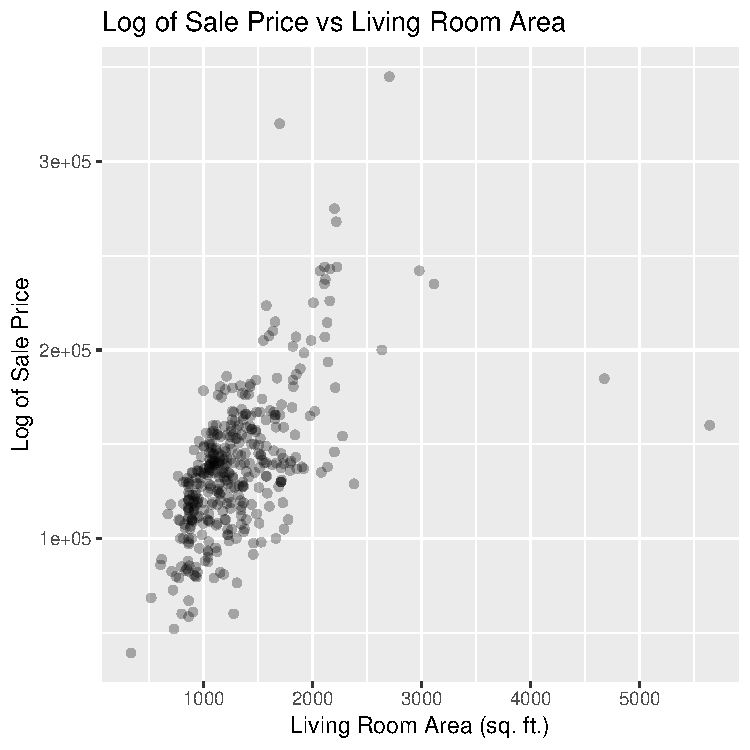
\includegraphics[width=0.45\linewidth]{HousePriceRegressionAnalysis_files/figure-latex/scatter-plot-1} 

}

\caption{Scatter Plot of Sale Price vs Living Room Area}\label{fig:scatter-plot}
\end{figure}

The images below show the scatter plots of log sale price vs living room
area (Figure \ref{fig:scatter-plots}). In the image on the right, the
scatter plot is shown for each neighborhood. In the image on the left
the observations for all three neighborhoods are included. In all cases,
a linear model appears to be reasonable to model this data.

\begin{figure}[htbp]

{\centering 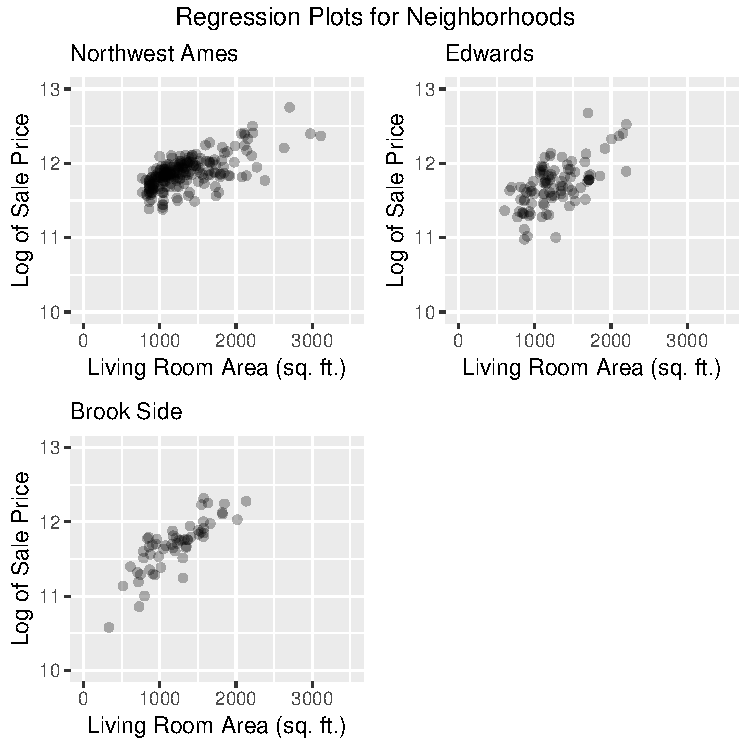
\includegraphics[width=0.45\linewidth]{HousePriceRegressionAnalysis_files/figure-latex/scatter-plots-1} 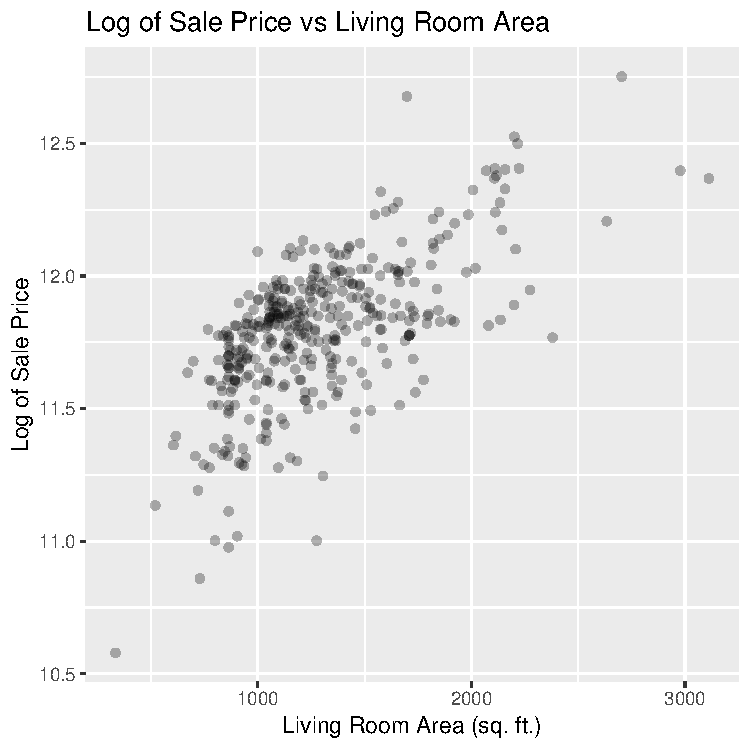
\includegraphics[width=0.45\linewidth]{HousePriceRegressionAnalysis_files/figure-latex/scatter-plots-2} 

}

\caption{Scatter Plots of Log of Sale Price vs Living Room Area}\label{fig:scatter-plots}
\end{figure}

\hypertarget{analysis-of-influential-points}{%
\subsection{Analysis of Influential
points}\label{analysis-of-influential-points}}

\label{appendix:infleu-points}

The two outlying observations with living room areas greater than 4000
sq. ft. appear to be from a different distribution than the main
dataset. Since these are partial sales, it is possible that the sale
prices do not reflect market value. For this reason, we will limit the
analysis to properities with less than 3500 sq. ft.
\ref{fig:infleu-points}

\begin{figure}[htbp]

{\centering 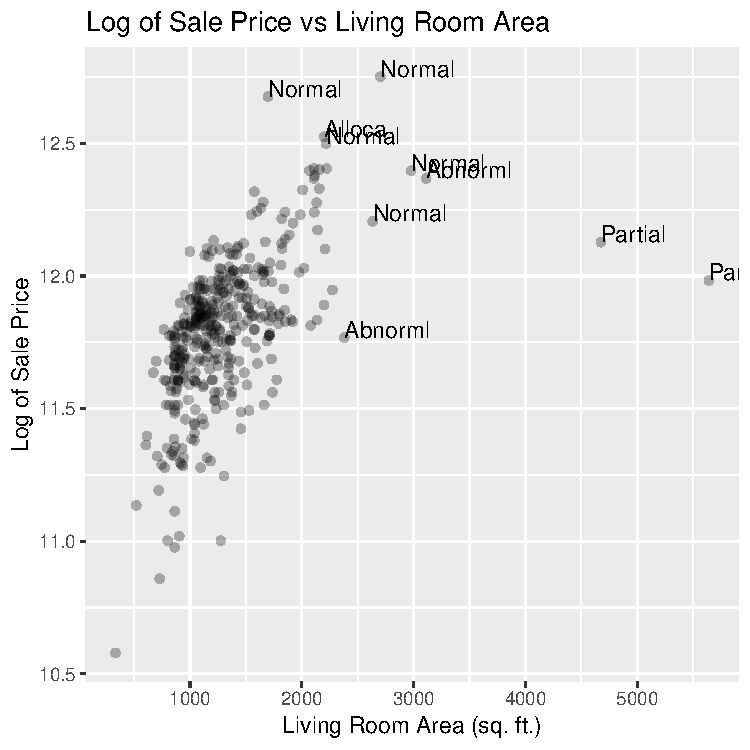
\includegraphics[width=0.5\linewidth]{HousePriceRegressionAnalysis_files/figure-latex/infleu-points-1} 

}

\caption{Influential Points}\label{fig:infleu-points}
\end{figure}

\newpage

\hypertarget{r-code-for-analysis-1}{%
\subsection{R Code For Analysis 1}\label{r-code-for-analysis-1}}

\begin{Shaded}
\begin{Highlighting}[]
\CommentTok{### Compuational Setup}
\CommentTok{# libraries}
\KeywordTok{library}\NormalTok{(knitr)}
\KeywordTok{library}\NormalTok{(kableExtra)}
\KeywordTok{library}\NormalTok{(tidyverse)}
\KeywordTok{library}\NormalTok{(olsrr)}
\KeywordTok{library}\NormalTok{(gridExtra)}
\KeywordTok{library}\NormalTok{(caret)}
\KeywordTok{library}\NormalTok{(multcomp)}

\CommentTok{# load data}
\NormalTok{train <-}\StringTok{ }\KeywordTok{read_csv}\NormalTok{(}\StringTok{'./data/train.csv'}\NormalTok{)}
\NormalTok{test <-}\StringTok{ }\KeywordTok{read_csv}\NormalTok{(}\StringTok{'./data/test.csv'}\NormalTok{)}

\CommentTok{# set a random seed for repodicibility}
\KeywordTok{set.seed}\NormalTok{(}\DecValTok{123}\NormalTok{)}

\CommentTok{### Helper Code}

\CommentTok{#' Print Typical Regression Fit Plots}
\CommentTok{#' }
\CommentTok{#' @description}
\CommentTok{#' Plots QQ plot of residuals, histogram of residuals,}
\CommentTok{#' residuals vs predicted values, and studentized }
\CommentTok{#' residuals vs predicted values. Depends on tidyverse}
\CommentTok{#' and gridExtra packages being loaded.}
\CommentTok{#'}
\CommentTok{#' @param data The true values corresponding to the input.}
\CommentTok{#' @param model The predicted/fitted values of the model.}
\NormalTok{basic.fit.plots <-}\StringTok{ }\ControlFlowTok{function}\NormalTok{(data, model) \{}
    
    \CommentTok{# depends on}
    \KeywordTok{require}\NormalTok{(tidyverse)}
    \KeywordTok{require}\NormalTok{(gridExtra)}

    \CommentTok{# get predicted values}
\NormalTok{    data}\OperatorTok{$}\NormalTok{Predicted <-}\StringTok{ }\KeywordTok{predict}\NormalTok{(model, data)}
    \CommentTok{# get residuals}
\NormalTok{    data}\OperatorTok{$}\NormalTok{Resid <-}\StringTok{ }\NormalTok{model}\OperatorTok{$}\NormalTok{residuals}
    \CommentTok{# get studentized residuals}
\NormalTok{    data}\OperatorTok{$}\NormalTok{RStudent <-}\StringTok{ }\KeywordTok{rstudent}\NormalTok{(}\DataTypeTok{model =}\NormalTok{ model)}

    \CommentTok{# create qqplot of residuals with reference line}
\NormalTok{    qqplot.resid <-}\StringTok{ }\NormalTok{data }\OperatorTok\StringTok{ }
\StringTok{      }\KeywordTok{ggplot}\NormalTok{(}\KeywordTok{aes}\NormalTok{(}\DataTypeTok{sample =}\NormalTok{ Resid)) }\OperatorTok{+}
\StringTok{      }\KeywordTok{geom_qq}\NormalTok{() }\OperatorTok{+}\StringTok{ }\KeywordTok{geom_qq_line}\NormalTok{() }\OperatorTok{+}
\StringTok{      }\KeywordTok{labs}\NormalTok{(}\DataTypeTok{subtitle =} \StringTok{'QQ Plot of Residuals'}\NormalTok{,}
           \DataTypeTok{x =} \StringTok{'Theoretical Quantile'}\NormalTok{,}
           \DataTypeTok{y =} \StringTok{'Acutal Quantile'}\NormalTok{)}
    
    \CommentTok{# create histogram of residuals}
\NormalTok{    hist.resid <-}\StringTok{ }\NormalTok{data }\OperatorTok\StringTok{ }
\StringTok{      }\KeywordTok{ggplot}\NormalTok{(}\KeywordTok{aes}\NormalTok{(}\DataTypeTok{x =}\NormalTok{ Resid)) }\OperatorTok{+}
\StringTok{      }\KeywordTok{geom_histogram}\NormalTok{(}\DataTypeTok{bins =} \DecValTok{15}\NormalTok{) }\OperatorTok{+}\StringTok{ }
\StringTok{      }\KeywordTok{labs}\NormalTok{(}\DataTypeTok{subtitle =} \StringTok{'Histogram of Residuals'}\NormalTok{,}
           \DataTypeTok{x =} \StringTok{'Residuals'}\NormalTok{,}
           \DataTypeTok{y =} \StringTok{'Count'}\NormalTok{)}

    \CommentTok{# create scatter plot of residuals vs predicted values}
\NormalTok{    resid.vs.pred <-}\StringTok{ }\NormalTok{data }\OperatorTok\StringTok{ }
\StringTok{      }\KeywordTok{ggplot}\NormalTok{(}\KeywordTok{aes}\NormalTok{(}\DataTypeTok{x =}\NormalTok{ Predicted, }\DataTypeTok{y =}\NormalTok{ Resid)) }\OperatorTok{+}
\StringTok{      }\KeywordTok{geom_point}\NormalTok{() }\OperatorTok{+}
\StringTok{      }\KeywordTok{geom_abline}\NormalTok{(}\DataTypeTok{slope =} \DecValTok{0}\NormalTok{) }\OperatorTok{+}\StringTok{ }
\StringTok{      }\KeywordTok{labs}\NormalTok{(}\DataTypeTok{subtitle =} \StringTok{'Residuals vs Prediction'}\NormalTok{,}
           \DataTypeTok{x =} \StringTok{'Predicted Value'}\NormalTok{,}
           \DataTypeTok{y =} \StringTok{'Residual'}\NormalTok{)}

    \CommentTok{# create scatter plot of studentized }
    \CommentTok{# residuals vs predicted values}
\NormalTok{    rStud.vs.pred <-}\StringTok{ }\NormalTok{data }\OperatorTok\StringTok{ }
\StringTok{      }\KeywordTok{ggplot}\NormalTok{(}\KeywordTok{aes}\NormalTok{(}\DataTypeTok{x =}\NormalTok{ Predicted, }\DataTypeTok{y =}\NormalTok{ RStudent)) }\OperatorTok{+}
\StringTok{      }\KeywordTok{geom_point}\NormalTok{() }\OperatorTok{+}
\StringTok{      }\KeywordTok{geom_abline}\NormalTok{(}\DataTypeTok{slope =} \DecValTok{0}\NormalTok{) }\OperatorTok{+}\StringTok{ }
\StringTok{      }\KeywordTok{geom_abline}\NormalTok{(}\DataTypeTok{slope =} \DecValTok{0}\NormalTok{, }\DataTypeTok{intercept =} \DecValTok{-2}\NormalTok{) }\OperatorTok{+}\StringTok{ }
\StringTok{      }\KeywordTok{geom_abline}\NormalTok{(}\DataTypeTok{slope =} \DecValTok{0}\NormalTok{, }\DataTypeTok{intercept =} \DecValTok{2}\NormalTok{) }\OperatorTok{+}\StringTok{ }
\StringTok{      }\KeywordTok{labs}\NormalTok{(}\DataTypeTok{subtitle =} \StringTok{'RStudent vs Prediction'}\NormalTok{,}
           \DataTypeTok{x =} \StringTok{'Predicted Value'}\NormalTok{,}
           \DataTypeTok{y =} \StringTok{'RStudent'}\NormalTok{)}
    
    \CommentTok{# add all four plots to grid as}
    \CommentTok{# qqplot           histogram}
    \CommentTok{# resid vs pred    RStud vs pred}
    \KeywordTok{grid.arrange}\NormalTok{(qqplot.resid,}
\NormalTok{             hist.resid,}
\NormalTok{             resid.vs.pred,}
\NormalTok{             rStud.vs.pred, }
             \DataTypeTok{nrow =} \DecValTok{2}\NormalTok{,}
             \DataTypeTok{top =} \StringTok{'Fit Assessment Plots'}\NormalTok{)}
\NormalTok{\}}

\CommentTok{#' Creates dummy variables (columns) for given column}
\CommentTok{#'}
\CommentTok{#' @param data A dataframe.}
\CommentTok{#' @param column A categorical column in data.}
\CommentTok{#' @param reference A value in the column to use a reference.}
\CommentTok{#' @param as.onehot Set to TRUE to use onehot encoding.}
\CommentTok{#'}
\NormalTok{get.dummies <-}\StringTok{ }\ControlFlowTok{function}\NormalTok{(data, column, reference, }\DataTypeTok{as.onehot =} \OtherTok{FALSE}\NormalTok{) \{}
  \CommentTok{# get the levels of the factor in column}
\NormalTok{  lev <-}\StringTok{ }\KeywordTok{levels}\NormalTok{(data[[column]])}
  \CommentTok{# do not remove reference for onehot encoding}
  \ControlFlowTok{if}\NormalTok{ (}\OperatorTok{!}\NormalTok{as.onehot) \{}
    \CommentTok{# remove the reference value}
\NormalTok{    lev <-}\StringTok{ }\NormalTok{lev[lev }\OperatorTok{!=}\StringTok{ }\NormalTok{reference]}
\NormalTok{  \}}
  \CommentTok{# add encodings}
  \ControlFlowTok{for}\NormalTok{ (fct }\ControlFlowTok{in}\NormalTok{ lev)\{}
\NormalTok{    new_col <-}\StringTok{ }\KeywordTok{paste}\NormalTok{(column, fct, }\DataTypeTok{sep =} \StringTok{'_'}\NormalTok{)}
\NormalTok{    data[new_col] <-}\StringTok{ }\KeywordTok{as.numeric}\NormalTok{(data[, column] }\OperatorTok{==}\StringTok{ }\NormalTok{fct)}
    \KeywordTok{print}\NormalTok{(new_col)}
\NormalTok{  \}}
\NormalTok{  data}
\NormalTok{\}}

\CommentTok{#' Calculates PRESS from `caret` CV model}
\CommentTok{#'}
\CommentTok{#' @param model.cv Calculates press from a model }
\CommentTok{#' produced by `caret`}
\CommentTok{#'}
\NormalTok{PRESS.cv <-}\StringTok{ }\ControlFlowTok{function}\NormalTok{(model.cv) \{}
\NormalTok{  meanN <-}\StringTok{ }\DecValTok{0}
\NormalTok{  folds <-}\StringTok{ }\NormalTok{model.cv}\OperatorTok{$}\NormalTok{control}\OperatorTok{$}\NormalTok{index}
  \ControlFlowTok{for}\NormalTok{ (i }\ControlFlowTok{in} \KeywordTok{seq}\NormalTok{(}\DecValTok{1}\OperatorTok{:}\KeywordTok{length}\NormalTok{(folds)))\{}
\NormalTok{    meanN <-}\StringTok{ }\NormalTok{meanN }\OperatorTok{+}\StringTok{ }\KeywordTok{length}\NormalTok{(folds[[i]])}
\NormalTok{  \}}
\NormalTok{  meanN <-}\StringTok{ }\NormalTok{meanN }\OperatorTok{/}\StringTok{ }\KeywordTok{length}\NormalTok{(folds)}
\NormalTok{  meanN }\OperatorTok{*}\StringTok{ }\NormalTok{((model.cv}\OperatorTok{$}\NormalTok{results}\OperatorTok{$}\NormalTok{RMSE)}\OperatorTok{^}\DecValTok{2}\NormalTok{)}
\NormalTok{\}}

\CommentTok{### plots of log of sale price ~ living room area}

\CommentTok{# create scatter plot for northwest ames}
\NormalTok{regplot.names <-}\StringTok{ }\NormalTok{train }\OperatorTok\StringTok{ }\KeywordTok{filter}\NormalTok{(Neighborhood }\OperatorTok{==}\StringTok{ 'NAmes'}\NormalTok{) }\OperatorTok
\StringTok{  }\KeywordTok{ggplot}\NormalTok{(}\KeywordTok{aes}\NormalTok{(}\DataTypeTok{x =}\NormalTok{ (GrLivArea), }\DataTypeTok{y =} \KeywordTok{log}\NormalTok{(SalePrice))) }\OperatorTok{+}
\StringTok{  }\KeywordTok{geom_point}\NormalTok{(}\DataTypeTok{alpha =} \FloatTok{0.3}\NormalTok{) }\OperatorTok{+}
\StringTok{  }\KeywordTok{ylim}\NormalTok{(}\DecValTok{10}\NormalTok{, }\DecValTok{13}\NormalTok{) }\OperatorTok{+}
\StringTok{  }\KeywordTok{xlim}\NormalTok{(}\DecValTok{0}\NormalTok{, }\DecValTok{3500}\NormalTok{) }\OperatorTok{+}
\StringTok{  }\KeywordTok{labs}\NormalTok{(}\DataTypeTok{subtitle =} \StringTok{'Northwest Ames'}\NormalTok{, }
       \DataTypeTok{y =} \StringTok{'Log of Sale Price'}\NormalTok{, }\DataTypeTok{x =} \StringTok{'Living Room Area (sq. ft.)'}\NormalTok{)}

\CommentTok{# create scatter plot for edwards}
\NormalTok{regplot.ed <-}\StringTok{ }\NormalTok{train }\OperatorTok
\StringTok{  }\KeywordTok{filter}\NormalTok{(GrLivArea }\OperatorTok{<}\StringTok{ }\DecValTok{4000}\NormalTok{) }\OperatorTok
\StringTok{  }\KeywordTok{filter}\NormalTok{(Neighborhood }\OperatorTok{==}\StringTok{ 'Edwards'}\NormalTok{) }\OperatorTok
\StringTok{  }\KeywordTok{ggplot}\NormalTok{(}\KeywordTok{aes}\NormalTok{(}\DataTypeTok{x =}\NormalTok{ (GrLivArea), }\DataTypeTok{y =} \KeywordTok{log}\NormalTok{(SalePrice))) }\OperatorTok{+}
\StringTok{  }\KeywordTok{geom_point}\NormalTok{(}\DataTypeTok{alpha =} \FloatTok{0.3}\NormalTok{) }\OperatorTok{+}
\StringTok{  }\KeywordTok{ylim}\NormalTok{(}\DecValTok{10}\NormalTok{, }\DecValTok{13}\NormalTok{) }\OperatorTok{+}
\StringTok{  }\KeywordTok{xlim}\NormalTok{(}\DecValTok{0}\NormalTok{, }\DecValTok{3500}\NormalTok{) }\OperatorTok{+}
\StringTok{  }\KeywordTok{labs}\NormalTok{(}\DataTypeTok{subtitle =} \StringTok{'Edwards'}\NormalTok{, }
       \DataTypeTok{y =} \StringTok{'Log of Sale Price'}\NormalTok{, }\DataTypeTok{x =} \StringTok{'Living Room Area (sq. ft.)'}\NormalTok{)}

\CommentTok{# create regression plot for brookside}
\NormalTok{regplot.brk <-}\StringTok{ }\NormalTok{train }\OperatorTok\StringTok{ }\KeywordTok{filter}\NormalTok{(Neighborhood }\OperatorTok{==}\StringTok{ 'BrkSide'}\NormalTok{) }\OperatorTok
\StringTok{  }\KeywordTok{ggplot}\NormalTok{(}\KeywordTok{aes}\NormalTok{(}\DataTypeTok{x =}\NormalTok{ (GrLivArea), }\DataTypeTok{y =} \KeywordTok{log}\NormalTok{(SalePrice))) }\OperatorTok{+}
\StringTok{  }\KeywordTok{geom_point}\NormalTok{(}\DataTypeTok{alpha =} \FloatTok{0.3}\NormalTok{) }\OperatorTok{+}
\StringTok{  }\KeywordTok{ylim}\NormalTok{(}\DecValTok{10}\NormalTok{, }\DecValTok{13}\NormalTok{) }\OperatorTok{+}
\StringTok{  }\KeywordTok{xlim}\NormalTok{(}\DecValTok{0}\NormalTok{, }\DecValTok{3500}\NormalTok{) }\OperatorTok{+}
\StringTok{  }\KeywordTok{labs}\NormalTok{(}\DataTypeTok{subtitle =} \StringTok{'Brook Side'}\NormalTok{, }
       \DataTypeTok{y =} \StringTok{'Log of Sale Price'}\NormalTok{, }\DataTypeTok{x =} \StringTok{'Living Room Area (sq. ft.)'}\NormalTok{)}

\CommentTok{# add the scatter plots for the neighborhood into a single plot}
\KeywordTok{grid.arrange}\NormalTok{(regplot.names,regplot.ed,regplot.brk, }\DataTypeTok{nrow =} \DecValTok{2}\NormalTok{,}
             \DataTypeTok{top =} \StringTok{'Regression Plots for Neighborhoods'}\NormalTok{)}

\CommentTok{# scatter plot of observations from all three neighborhoods}
\NormalTok{train }\OperatorTok\StringTok{ }
\StringTok{  }\KeywordTok{filter}\NormalTok{(GrLivArea }\OperatorTok{<}\StringTok{ }\DecValTok{4000}\NormalTok{) }\OperatorTok
\StringTok{  }\KeywordTok{ggplot}\NormalTok{(}\KeywordTok{aes}\NormalTok{(}\DataTypeTok{x =}\NormalTok{ (GrLivArea), }\DataTypeTok{y =} \KeywordTok{log}\NormalTok{(SalePrice))) }\OperatorTok{+}
\StringTok{  }\KeywordTok{geom_point}\NormalTok{(}\DataTypeTok{alpha =} \FloatTok{0.3}\NormalTok{) }\OperatorTok{+}
\StringTok{  }\KeywordTok{labs}\NormalTok{(}\DataTypeTok{title =} \StringTok{'Log of Sale Price vs Living Room Area'}\NormalTok{, }
       \DataTypeTok{y =} \StringTok{'Log of Sale Price'}\NormalTok{, }\DataTypeTok{x =} \StringTok{'Living Room Area (sq. ft.)'}\NormalTok{)}

\CommentTok{### Filter data for analysis 1}

\NormalTok{train <-}\StringTok{ }\NormalTok{train }\OperatorTok\StringTok{ }
\StringTok{  }\KeywordTok{filter}\NormalTok{(Neighborhood }\OperatorTok\StringTok{ }\KeywordTok{c}\NormalTok{(}\StringTok{"Edwards"}\NormalTok{, }\StringTok{"BrkSide"}\NormalTok{, }\StringTok{"NAmes"}\NormalTok{))}
\NormalTok{train}\OperatorTok{$}\NormalTok{Neighborhood <-}\StringTok{ }\KeywordTok{as.factor}\NormalTok{(train}\OperatorTok{$}\NormalTok{Neighborhood)}

\CommentTok{# create dummy variables with Neighborhood == 'Edwards' as reference}
\NormalTok{train <-}\StringTok{ }\KeywordTok{get.dummies}\NormalTok{(train, }\StringTok{"Neighborhood"}\NormalTok{, }\DataTypeTok{reference =} \StringTok{'Edwards'}\NormalTok{)}

\CommentTok{# remove suspect points from training data}
\NormalTok{train.mod <-}\StringTok{ }\NormalTok{train }\OperatorTok\StringTok{ }\KeywordTok{filter}\NormalTok{(GrLivArea }\OperatorTok{<}\StringTok{ }\DecValTok{4000}\NormalTok{)}

\CommentTok{#### Extra Sum of Squares}

\CommentTok{# full model formula}
\NormalTok{model.formula =}\StringTok{ }\KeywordTok{log}\NormalTok{(SalePrice) }\OperatorTok{~}\StringTok{ }\NormalTok{(GrLivArea) }\OperatorTok{+}\StringTok{ }
\StringTok{     }\NormalTok{Neighborhood_BrkSide }\OperatorTok{+}\StringTok{ }
\StringTok{     }\NormalTok{Neighborhood_NAmes }\OperatorTok{+}
\StringTok{     }\NormalTok{(GrLivArea) }\OperatorTok{*}\StringTok{ }\NormalTok{Neighborhood_BrkSide }\OperatorTok{+}\StringTok{ }
\StringTok{     }\NormalTok{(GrLivArea) }\OperatorTok{*}\StringTok{ }\NormalTok{Neighborhood_NAmes}
\CommentTok{# reduced model formula}
\NormalTok{model.reduced.formula =}\StringTok{ }\KeywordTok{log}\NormalTok{(SalePrice) }\OperatorTok{~}\StringTok{ }\NormalTok{(GrLivArea) }\OperatorTok{+}\StringTok{ }
\StringTok{     }\NormalTok{Neighborhood_BrkSide }\OperatorTok{+}\StringTok{ }
\StringTok{     }\NormalTok{Neighborhood_NAmes}

\CommentTok{# fit models}
\NormalTok{model <-}\StringTok{ }\KeywordTok{lm}\NormalTok{(}\DataTypeTok{formula =}\NormalTok{ model.formula, }\DataTypeTok{data =}\NormalTok{ train.mod)}
\NormalTok{model.reduced <-}\StringTok{ }\KeywordTok{lm}\NormalTok{(}\DataTypeTok{formula =}\NormalTok{ model.reduced.formula, }\DataTypeTok{data =}\NormalTok{ train.mod)}
\CommentTok{# ESS test on models}
\KeywordTok{anova}\NormalTok{(model.reduced, model)}

\CommentTok{### Assessment plots}

\CommentTok{# create plots of residuals}
\KeywordTok{basic.fit.plots}\NormalTok{(train.mod, model)}
\CommentTok{# create leverage / outlier plot}
\KeywordTok{ols_plot_resid_lev}\NormalTok{(model)}

\CommentTok{### cross validation}

\CommentTok{## cross validate the full model}

\CommentTok{# Set up repeated k-fold cross-validation}
\NormalTok{train.control <-}\StringTok{ }\KeywordTok{trainControl}\NormalTok{(}\DataTypeTok{method =} \StringTok{"cv"}\NormalTok{, }\DataTypeTok{number =} \DecValTok{10}\NormalTok{)}
\CommentTok{# Train the model}
\NormalTok{model.cv <-}\StringTok{ }\KeywordTok{train}\NormalTok{(model.formula, }
                    \DataTypeTok{data =}\NormalTok{ train.mod,}
                    \DataTypeTok{method =} \StringTok{'lm'}\NormalTok{,}
                    \DataTypeTok{trControl =}\NormalTok{ train.control)}
\CommentTok{# print model summary}
\NormalTok{model.cv}

\CommentTok{# get the CV results}
\NormalTok{res <-}\StringTok{ }\NormalTok{model.cv}\OperatorTok{$}\NormalTok{results}

\CommentTok{# get cross-validated PRESS statistic}
\NormalTok{PCV <-}\StringTok{ }\KeywordTok{PRESS.cv}\NormalTok{(model.cv)}

\CommentTok{## cross validate the reduced model}

\CommentTok{# Set up repeated k-fold cross-validation}
\NormalTok{train.control <-}\StringTok{ }\KeywordTok{trainControl}\NormalTok{(}\DataTypeTok{method =} \StringTok{"cv"}\NormalTok{, }\DataTypeTok{number =} \DecValTok{10}\NormalTok{)}
\CommentTok{# Train the model}
\NormalTok{model.reduced.cv <-}\StringTok{ }\KeywordTok{train}\NormalTok{(model.reduced.formula, }
                    \DataTypeTok{data =}\NormalTok{ train.mod,}
                    \DataTypeTok{method =} \StringTok{'lm'}\NormalTok{,}
                    \DataTypeTok{trControl =}\NormalTok{ train.control)}
\CommentTok{# print model summary}
\NormalTok{model.reduced.cv}

\CommentTok{# get the CV results}
\NormalTok{res.red <-}\StringTok{ }\NormalTok{model.reduced.cv}\OperatorTok{$}\NormalTok{results}

\CommentTok{# get cross-validated PRESS statistic}
\NormalTok{PCV.red <-}\StringTok{ }\KeywordTok{PRESS.cv}\NormalTok{(model.reduced.cv)}

\CommentTok{# print accuracy metrics to md table}
\KeywordTok{kable}\NormalTok{(}\KeywordTok{data.frame}\NormalTok{(}\StringTok{'Model'}\NormalTok{ =}\StringTok{ }\KeywordTok{c}\NormalTok{(}\StringTok{'Full Model'}\NormalTok{, }\StringTok{'Reduced Model'}\NormalTok{), }
                 \StringTok{'RMSE'}\NormalTok{=}\KeywordTok{c}\NormalTok{(res}\OperatorTok{$}\NormalTok{RMSE, res.red}\OperatorTok{$}\NormalTok{RMSE),}
                 \StringTok{'CV Press'}\NormalTok{=}\KeywordTok{c}\NormalTok{(PCV, PCV.red),}
                 \StringTok{'Adjused R Squared'}\NormalTok{=}\KeywordTok{c}\NormalTok{(res}\OperatorTok{$}\NormalTok{Rsquared, res.red}\OperatorTok{$}\NormalTok{Rsquared)),}
      \StringTok{"latex"}\NormalTok{, }\DataTypeTok{booktabs =}\NormalTok{ T)  }\OperatorTok
\StringTok{  }\KeywordTok{kable_styling}\NormalTok{(}\DataTypeTok{position =} \StringTok{"center"}\NormalTok{)}

\CommentTok{### get the parameters from the CV'ed model}

\CommentTok{# extract the model estimates from the model summary}
\NormalTok{sm <-}\StringTok{ }\KeywordTok{summary}\NormalTok{(model)}
\NormalTok{sm.coe <-}\StringTok{ }\NormalTok{sm}\OperatorTok{$}\NormalTok{coefficients}
\CommentTok{# get the CIs for the coefficients}
\NormalTok{model.conf <-}\StringTok{ }\KeywordTok{confint}\NormalTok{(model)}

\CommentTok{# print model estimates to md / latex table}
\CommentTok{# extract the params and put into a dataframe}
\KeywordTok{kable}\NormalTok{(}\KeywordTok{data.frame}\NormalTok{(}\StringTok{'Parameter'}\NormalTok{ =}\StringTok{ }\KeywordTok{c}\NormalTok{(}\StringTok{'Intercept'}\NormalTok{, }\StringTok{'GrLivArea'}\NormalTok{, }
                                 \StringTok{'Neighborhood_BrkSide'}\NormalTok{, }\StringTok{'Neighborhood_NAmes'}\NormalTok{, }
                                 \StringTok{'GrLivArea:Neighborhood_BrkSide'}\NormalTok{, }
                                 \StringTok{'GrLivArea:Neighborhood_NAmes '}\NormalTok{), }
                 \StringTok{'Estimate'}\NormalTok{=}\KeywordTok{c}\NormalTok{(sm.coe[[}\DecValTok{1}\NormalTok{]],sm.coe[[}\DecValTok{2}\NormalTok{]],sm.coe[[}\DecValTok{3}\NormalTok{]],}
\NormalTok{                              sm.coe[[}\DecValTok{4}\NormalTok{]],sm.coe[[}\DecValTok{5}\NormalTok{]],sm.coe[[}\DecValTok{6}\NormalTok{]]),}
                 \StringTok{'CI Lower'}\NormalTok{ =}\StringTok{ }\KeywordTok{c}\NormalTok{(model.conf[[}\DecValTok{1}\NormalTok{]],model.conf[[}\DecValTok{2}\NormalTok{]],model.conf[[}\DecValTok{3}\NormalTok{]],}
\NormalTok{                                model.conf[[}\DecValTok{4}\NormalTok{]],model.conf[[}\DecValTok{5}\NormalTok{]],model.conf[[}\DecValTok{6}\NormalTok{]]),}
                 \StringTok{'CI Upper'}\NormalTok{ =}\StringTok{ }\KeywordTok{c}\NormalTok{(model.conf[[}\DecValTok{1}\NormalTok{,}\DecValTok{2}\NormalTok{]],model.conf[[}\DecValTok{1}\NormalTok{,}\DecValTok{2}\NormalTok{]],model.conf[[}\DecValTok{3}\NormalTok{,}\DecValTok{2}\NormalTok{]],}
\NormalTok{                                model.conf[[}\DecValTok{4}\NormalTok{,}\DecValTok{2}\NormalTok{]],model.conf[[}\DecValTok{5}\NormalTok{,}\DecValTok{2}\NormalTok{]],model.conf[[}\DecValTok{6}\NormalTok{,}\DecValTok{2}\NormalTok{]])),}
      \StringTok{"latex"}\NormalTok{, }\DataTypeTok{booktabs =}\NormalTok{ T)  }\OperatorTok
\StringTok{  }\KeywordTok{kable_styling}\NormalTok{(}\DataTypeTok{position =} \StringTok{"center"}\NormalTok{)}

\CommentTok{# summary of model to get overall test}
\KeywordTok{summary}\NormalTok{(}\KeywordTok{lm}\NormalTok{(model.formula, }\DataTypeTok{data =}\NormalTok{ train.mod))}

\CommentTok{## Calculate CIs of slopes not in standard table}

\CommentTok{# get CI for Northwest Ames}
\KeywordTok{confint}\NormalTok{(}\KeywordTok{glht}\NormalTok{(model, }\DataTypeTok{linfct =} \StringTok{"GrLivArea + GrLivArea:Neighborhood_NAmes = 1"}\NormalTok{))}

\CommentTok{# get CI for Brookside}
\KeywordTok{confint}\NormalTok{(}\KeywordTok{glht}\NormalTok{(model, }\DataTypeTok{linfct =} \StringTok{"GrLivArea + GrLivArea:Neighborhood_BrkSide = 1"}\NormalTok{))}
\end{Highlighting}
\end{Shaded}

\hypertarget{r-code-for-analysis-2}{%
\subsection{R Code For Analysis 2}\label{r-code-for-analysis-2}}

Include ``well commented'' \texttt{code} in the appendex!

\begin{Shaded}
\begin{Highlighting}[]
\NormalTok{train }\OperatorTok\StringTok{ }\KeywordTok{ggplot}\NormalTok{(}\KeywordTok{aes}\NormalTok{(}\DataTypeTok{x =}\NormalTok{ (GrLivArea), }\DataTypeTok{y =} \KeywordTok{log}\NormalTok{(SalePrice))) }\OperatorTok{+}
\StringTok{  }\KeywordTok{geom_point}\NormalTok{(}\DataTypeTok{alpha =} \FloatTok{0.3}\NormalTok{) }\OperatorTok{+}
\StringTok{  }\KeywordTok{labs}\NormalTok{(}\DataTypeTok{title =} \StringTok{'Log of Sale Price vs Living Room Area'}\NormalTok{, }
       \DataTypeTok{y =} \StringTok{'Log of Sale Price'}\NormalTok{, }\DataTypeTok{x =} \StringTok{'Living Room Area'}\NormalTok{) }\OperatorTok{+}
\StringTok{  }\KeywordTok{geom_text}\NormalTok{(}\KeywordTok{aes}\NormalTok{(}\DataTypeTok{label =} \KeywordTok{ifelse}\NormalTok{((}\KeywordTok{log}\NormalTok{(GrLivArea) }\OperatorTok{>}\StringTok{ }\FloatTok{7.75} \OperatorTok{&}\StringTok{ }\KeywordTok{log}\NormalTok{(SalePrice) }\OperatorTok{>}\StringTok{ }\DecValTok{11}\NormalTok{) }\OperatorTok{|}
\StringTok{                                 }\NormalTok{(}\KeywordTok{log}\NormalTok{(SalePrice) }\OperatorTok{>}\StringTok{ }\FloatTok{12.45}\NormalTok{),}
\NormalTok{                               SaleCondition, }\StringTok{''}\NormalTok{)), }\DataTypeTok{hjust=}\DecValTok{0}\NormalTok{, }\DataTypeTok{vjust=}\DecValTok{0}\NormalTok{)}
\end{Highlighting}
\end{Shaded}

\renewcommand\refname{References}
\bibliography{references.bib}


\end{document}
